% ------------------------------------------------------------------------
%
% -------------------      Plantilla_UIS.tex       -----------------------
%
% ------------------------------------------------------------------------
% ------------------------------------------------------------------------
% ------------------------------------------------------------------------
% Versión de plantilla para realización de informes de trabajo de grado
% construida para uso de la Universidad Industrial de Santander.
%
% Reservados todos los derechos
%
% Bucaramanga, Colombia
%
% Febrero 03 de 2019
%
% ------------------------------------------------------------------------
% ------------------------------------------------------------------------
% ------------------------------------------------------------------------
%
% --------------------------\documentclass[letter,oneside,12pt,spanish]{report}

\documentclass[letter,oneside,12pt,spanish]{report}
% ------------------------------------------------------------------------
\usepackage{uislatexstyleAPA} % Libreria UIS APA
% ------------------------------------------------------------------------

% --- AQUÍ VAN TODOS LOS PAQUETES --- %
\usepackage[utf8]{inputenc}
\usepackage{epsfig}
\usepackage{amsmath}
\usepackage{amssymb}
\usepackage{graphicx}
\usepackage{float}
\usepackage{multirow}
\usepackage{wrapfig}
\usepackage{enumitem}
\usepackage{xcolor}
\usepackage{caption}
\usepackage{tcolorbox}
\usepackage{subfigure}
\usepackage{listings}
\usepackage{minted}
\usepackage{csquotes}
\usepackage[style=apa]{biblatex}
\usepackage{geometry}
\usepackage{hyperref}
\usepackage{pdfpages}
\usepackage{attachfile2}
\usepackage{setspace} 
\usepackage{pgffor}

% --- CONFIGURACIONES DE COLORES --- %
\definecolor{bg}{rgb}{0.95,0.95,0.92}
\definecolor{purple}{rgb}{0.5,0,0.5}
\definecolor{orange}{rgb}{0.9,0.4,0}
\definecolor{codeborder}{RGB}{0,0,0}
\definecolor{codebackground}{RGB}{255,255,255}
\definecolor{codegray}{RGB}{128,128,128}
\definecolor{codegreen}{RGB}{0,153,0}
\definecolor{codeorange}{RGB}{255,125,80}

% --- CONFIGURACIÓN DE LISTINGS --- %
\lstdefinestyle{mystyle}{
	frame=shadowbox,
	backgroundcolor=\color{codebackground},
	commentstyle=\color{codegray},
	keywordstyle=\color{codeorange},
	numberstyle=\tiny\color{codegray},
	stringstyle=\color{codegreen},
	basicstyle=\ttfamily\footnotesize,
	breakatwhitespace=false,
	breaklines=true,
	captionpos=b,
	keepspaces=true,
	numbers=none,
	showspaces=false,
	showstringspaces=false,
	showtabs=false,
	tabsize=2,
	frame=single,
	rulecolor=\color{codeborder},
	framesep=4pt,
	xleftmargin=10pt,
	xrightmargin=10pt,
}
\lstset{style=mystyle}

% --- OTRAS CONFIGURACIONES --- %
\addbibresource{biblio.bib}
\geometry{headheight=15.13202pt}
\captionsetup[figure]{labelfont={bf}, singlelinecheck=false}
\parskip=12pt

\begin{document}                              % Inicio de documento
% ------------------------------------------------------------------------
% Definición silábica de palabras
% ------------------------------------------------------------------------
% \hyphenation{pro-por-cio-nal di-se-ño}
\hypersetup {pdfborder = {0 0 0}}
% ------------------------------------------------------------------------
% Titulo resumido del trabajo que aparecerá en cornisa
% ------------------------------------------------------------------------
\title{AMBIENTE DE APRENDIZAJE PARA LA ENSEÑANZA DE ESTADÍSTICA II}
% ------------------------------------------------------------------------
% Elementos previos al contenido del trabajo
% ------------------------------------------------------------------------ 

\begin{center}

Ambiente de aprendizaje para la enseñanza de Estadística II: un enfoque en teoría, prácticas y autoevaluación\vspace{1.5cm}

Jorge Eduardo Suárez Cortés\\
Daniel Alejandro Sánchez Rodríguez \\ \vspace{1.5cm}

Trabajo de Grado para optar al título de Ingeniero de Sistemas\\ \vspace{1.5cm}

Director\\
Andrés Leonardo González Gómez\\
PhD (c). Ciencias de la Computación\vspace{1.5cm}


Universidad Industrial de Santander\\
Facultad de Ingenierías Fisicomecánicas\\
Escuela de Ingeniería de Sistemas e Informática\\
Ingeniería de Sistemas\\
Bucaramanga\\
2025\\

\end{center}

% Portadilla

\parskip=0pt

\newpage

\titlecontents{paragraph}[0em]{\normalfont\normalsize}{\thecontentslabel. }{}{\titlerule*[1em]{}\contentspage}



\parskip=12pt
\tableofcontents                    

% Tabla de contenido
% ------------------------------------------------------------------------
\newpage

\listoffigures                         % Lista de figuras, tablas y anexos
\newpage

\chapter*{Glosario}

\begin{description}

\item \textbf{Ambiente Virtual de Aprendizaje (AVA)}: Entorno digital que integra recursos, actividades y herramientas interactivas para apoyar los procesos de enseñanza y aprendizaje en línea o semipresenciales.
\item \textbf{Autoevaluación}: Estrategia pedagógica que permite a los estudiantes valorar su propio proceso de aprendizaje mediante actividades de retroalimentación automática.
\item \textbf{Backend}: Parte de una aplicación o sistema que gestiona la lógica del negocio, la base de datos y el procesamiento interno, generalmente ejecutada en el servidor y no visible para el usuario final.
\item \textbf{Base de datos}: Conjunto estructurado de información almacenada de manera organizada que permite el acceso, la gestión y la actualización de datos académicos y de evaluación.
\item \textbf{Colab (Google Colaboratory)}: Plataforma en la nube de Google que permite ejecutar código en Python a través de notebooks, facilitando el aprendizaje automático, la programación y el análisis de datos sin necesidad de instalación local.
\item \textbf{Docker}: Plataforma de virtualización ligera que permite empaquetar aplicaciones y servicios en contenedores portátiles, facilitando su despliegue en diferentes entornos.
\item \textbf{Estadística inferencial}: Rama de la estadística que utiliza datos muestrales para realizar inferencias, estimaciones o pruebas sobre parámetros poblacionales.
\item \textbf{Frontend}: Parte visible de una aplicación con la que interactúa el usuario, compuesta por interfaces gráficas y elementos de diseño implementados en tecnologías como HTML, CSS y JavaScript.
\item \textbf{Genially}: Herramienta en línea para la creación de contenidos interactivos y visuales, como presentaciones, infografías y recursos educativos dinámicos.
\item \textbf{Grader}: En español se le denomina \textit{evaluador automático}, aunque el término más comúnmente usado en la literatura académica y técnica es \textit{Grader}. Autocalificador de evaluación que corrige ejercicios prácticos, especialmente de programación y estadística, generando resultados inmediatos. 
\item \textbf{H5P}: Framework de código abierto que permite crear, compartir y reutilizar contenidos interactivos, como cuestionarios, presentaciones y actividades educativas digitales.
\item \textbf{Jupyter Notebook}: Entorno interactivo de código abierto que permite crear y compartir documentos que contienen código en vivo, visualizaciones y texto explicativo, ampliamente usado en programación, análisis de datos y enseñanza.
\item \textbf{LMS (Learning Management System)}: Sistema de gestión del aprendizaje que permite planificar, implementar y evaluar procesos educativos en entornos virtuales. Facilita la creación de cursos, administración de contenidos, seguimiento del progreso de los estudiantes y la comunicación entre docentes y alumnos.
\item \textbf{Moodle}: Plataforma de gestión de aprendizaje (LMS, por sus siglas en inglés) de código abierto, utilizada para crear cursos en línea, administrar contenidos y facilitar la comunicación entre docentes y estudiantes.
\item \textbf{Nginx}: Servidor web y proxy inverso de alto rendimiento que se utiliza para distribuir carga, manejar conexiones concurrentes y servir aplicaciones web de manera eficiente.
\item \textbf{Node.js}: Entorno de ejecución de JavaScript orientado al desarrollo de aplicaciones web y servidores, utilizado para gestionar la comunicación entre sistemas del entorno virtual.
\item \textbf{Playit.gg}: Servicio que permite crear túneles seguros para acceder a aplicaciones locales desde internet, sin necesidad de configuraciones avanzadas en redes.
\item \textbf{SEB (Safe Exam Browser)}: Aplicación que bloquea el acceso a páginas web, programas y funciones del sistema durante una evaluación en línea, garantizando un entorno seguro y controlado para la presentación de exámenes.
\end{description}


% ------------------------------------------------------------------------
\newpage

% Contenido del Informe
% ------------------------------------------------------------------------
\newpage

\chapter*{Resumen}

\footnotesize{
\begin{description}
  \item[Título:] Ambiente de aprendizaje para la enseñanza de Estadística II: un enfoque en teoría, prácticas y autoevaluación.
  \astfootnote{Trabajo de grado}
  \item[Autores:] Jorge Eduardo Suárez Cortés y Daniel Alejandro Sánchez Rodríguez.
  \asttfootnote{Facultad de Ingenierías Fisicomecánicas. Escuela de Ingeniería de Sistemas e Informática.\\
  	Director: Andrés Leonardo González Gómez}
  \item[Palabras clave:] Ambiente virtual de aprendizaje, Moodle, Estadística II, Autoevaluación.
  \item[Descripción:] {
    \begin{spacing}{1.7}
    El presente trabajo de grado describe el diseño, desarrollo e implementación de un ambiente de aprendizaje virtual para la asignatura Estadística II, dirigida a estudiantes de la Escuela de Ingeniería de Sistemas e Informática de la Universidad Industrial de Santander. El ambiente fue construido sobre la plataforma Moodle, con el objetivo de ofrecer una experiencia de aprendizaje más activa, significativa y continua mediante la integración sistemática de un plan de aula modular que articula contenidos teóricos, ejercicios prácticos en Python y R a través de Colab Notebooks e instrumentos de evaluación formativa, tales como evaluaciones con calificación automática y retroalimentación inmediata.  
    El enfoque pedagógico del entorno se basa en el aprendizaje activo y la construcción progresiva del conocimiento, promoviendo la participación continua del estudiante y el desarrollo de competencias relacionadas con el análisis estadístico y la interpretación de datos. Las actividades propuestas están diseñadas para favorecer la autonomía del aprendizaje. Los resultados obtenidos sugieren que el uso del ambiente virtual contribuye a mejorar la comprensión de los contenidos estadísticos, lo cual se evidencia en la evolución positiva de las calificaciones en las cinco prácticas de laboratorio donde se observó un aumento progresivo en los promedios y una disminución en la varianza de los resultados, así como en los hallazgos de la encuesta aplicada a los estudiantes, en la cual más del 80\% manifestó que la integración de prácticas en Colab y evaluaciones automáticas favoreció su proceso de aprendizaje.  
    Esta propuesta representa una alternativa metodológica y tecnológica que responde a las necesidades actuales de la educación superior en el ámbito de la ingeniería de sistemas, especialmente en contextos donde la articulación entre teoría y práctica resulta esencial para el desarrollo de competencias profesionales.
    \end{spacing}
  }
\end{description}}\normalsize


% ------------------------------------------------------------------------

\newpage

\chapter*{Abstract}

\footnotesize{
\begin{description}
  \item[Title:] Learning Environment for the Teaching of Statistics II: A Focus on Theory, Practice, and Self-Assessment.
  \astfootnote{Degree Work}
  \item[Authors:] Jorge Eduardo Suárez Cortés y Daniel Alejandro Sánchez Rodríguez.
  \asttfootnote{Faculty of Physicomechanical Engineering. School of Systems and Computer Engineering.\\
  	Director: Andrés Leonardo González Gómez}
  \item[Key words:] Virtual learning environment, Moodle, Statistics II, Self-assessment.
  \item[Description:] {
    \begin{spacing}{1.9}
	This work presents the design, development, and implementation of a virtual learning environment for the Statistics II course, aimed at students of the School of Systems Engineering and Computer Science at the Industrial University of Santander. The environment was built on the Moodle platform, with the aim of offering a more active, meaningful, and continuous learning experience through the systematic integration of a modular classroom plan that combines theoretical content, practical exercises in Python and R through Colab Notebooks, and formative assessment tools, such as automatically graded assessments and immediate feedback.  
	The pedagogical approach of the environment is based on active learning and the progressive construction of knowledge, promoting continuous student participation and the development of skills related to statistical analysis and data interpretation. The proposed activities are designed to encourage autonomous learning. The results obtained suggest that the use of the virtual environment contributes to improving the understanding of statistical content, as evidenced by the positive evolution of grades in the five laboratory practices, where a progressive increase in averages and a decrease in the variance of results were observed, as well as in the findings of the survey applied to students, in which more than 80\% stated that the integration of practices in Colab and automatic assessments favored their learning process.  
    This proposal represents a methodological and technological alternative that responds to the current needs of higher education in the field of systems engineering, especially in contexts where the articulation between theory and practice is essential for the development of professional skills.
	\end{spacing}
  }
\end{description}}\normalsize

% Abstract

% ------------------------------------------------------------------------
% Capítulos
% ------------------------------------------------------------------------
\newpage

\nnchapter{Introducción}

La enseñanza de la estadística en la educación superior, particularmente en los programas de ingeniería, constituye un desafío permanente debido a la necesidad de articular los fundamentos teóricos con la práctica aplicada y el desarrollo de competencias analíticas que respondan a problemas reales. En la asignatura Estadística II de la Escuela de Ingeniería de Sistemas e Informática de la Universidad Industrial de Santander, se han identificado dificultades recurrentes que se reflejan en la percepción de la estadística como un conjunto de procedimientos abstractos y poco vinculados con la práctica profesional. Esta situación repercute en bajos niveles de motivación, escasa apropiación de los contenidos y limitaciones en el aprendizaje autónomo.

Ante esta problemática, resulta necesario implementar estrategias pedagógicas que favorezcan un aprendizaje más activo, dinámico y significativo. En este sentido, los Ambientes Virtuales de Aprendizaje (AVA) se consolidan como una alternativa metodológica y tecnológica para complementar la enseñanza tradicional. Dichos entornos permiten integrar contenidos teóricos, actividades prácticas y mecanismos de evaluación formativa en un mismo espacio digital, promoviendo la autonomía del estudiante y su participación activa en el proceso educativo.
En concordancia con lo anterior, el presente trabajo de grado tuvo como propósito diseñar e implementar un ambiente de aprendizaje para la asignatura Estadística II, utilizando la plataforma Moodle como eje central para la gestión de contenidos y actividades académicas. A este entorno se integraron recursos computacionales basados en Google Colab, orientados al desarrollo de prácticas en Python y R, así como un sistema de autoevaluación mediante graders automatizados, lo cual permite validar en tiempo real las soluciones planteadas por los estudiantes y ofrecer retroalimentación inmediata.

Para soportar estas funcionalidades se implementó una arquitectura de microservicios que articula diversas tecnologías: Node.js para la gestión del backend, React para la interfaz de notas para el docente, MariaDB para la administración de datos académicos y Docker como plataforma de contenedorización que garantiza la portabilidad y el despliegue uniforme de los servicios. Adicionalmente, se empleó Playit.gg como servicio de túneles seguros, lo que posibilitó la exposición del servidor y el acceso remoto al sistema, asegurando así el funcionamiento de los procesos de calificación automática y retroalimentación en los graders de esta manera se consolidó un ecosistema tecnológico robusto y escalable.

El desarrollo del proyecto se llevó a cabo mediante una metodología ágil, organizada en sprints, que permitió estructurar de forma progresiva las fases de diseño, implementación e integración tecnológica. Asimismo, se realizó un pilotaje con dos grupos de estudiantes, lo cual facilitó la validación inicial de la propuesta en un contexto académico auténtico y permitió efectuar los ajustes necesarios para garantizar su pertinencia pedagógica y técnica.


% ------------------------------------------------------------------------

\newpage


\chapter{Objetivos}

\section{Objetivo General}

\begin{itemize}
    \item Diseñar y desarrollar un entorno virtual para la asignatura de Estadística II, de la Escuela de Ingeniería de Sistemas e 
    Informática de la UIS, que facilite la ejecución de un plan de aula propuesto para la práctica, el aprendizaje y la autoevaluación 
    del contenido de la asignatura, mediante herramientas de Python y R.
\end{itemize}

\section{Objetivos Específicos}

\begin{itemize}
    \item Diseñar un plan de aula modular para la asignatura Estadística II que organice los contenidos teóricos y prácticos en 
    unidades interactivas basadas en Colab Notebooks, Python y R, e incluya calificadores automáticos y ejercicios con retroalimentación 
    instantánea.
    
    \item Implementar un ambiente de aprendizaje virtual en la plataforma Moodle que integre las tecnologías definidas (Colab Notebooks, 
    Python y R) y organice los contenidos teóricos y prácticos junto con materiales didácticos de apoyo, consolidando una experiencia 
    formativa práctica y accesible para la asignatura Estadística II.
    
    \item Establecer instrumentos de medición para las actividades prácticas y autoevaluativas en Moodle (desarrolladas con Python y R), 
    que permitan medir el logro de los resultados de aprendizaje durante el desarrollo del proyecto en el curso de Estadística II.

    \item Pilotear el ambiente virtual de aprendizaje diseñado, con sus contenidos interactivos e instrumentos de evaluación, en por lo 
    menos dos grupos de Estadística II de la Escuela de Ingeniería de Sistemas e Informática de la UIS, para validar su 
    usabilidad, satisfacción y efectividad en el logro de los resultados de aprendizaje.

\end{itemize}

% ------------------------------------------------------------------------

\newpage

\chapter{Marco Teórico}

\section{Estadística}

La estadística constituye una herramienta fundamental en la ciencia, la ingeniería y la administración, al proporcionar métodos rigurosos para recopilar, organizar, presentar, analizar e interpretar datos para apoyar la toma de decisiones. En la actualidad, desempeña un papel crucial en el análisis de sistemas complejos, la mejora de procesos y el control de calidad en distintos entornos académicos, industriales y científicos.

De acuerdo con \textcite{montgomery1996}, la estadística moderna se divide en dos grandes áreas: estadística descriptiva y estadística inferencial. La primera se ocupa de técnicas que permiten resumir y describir de manera gráfica o numérica los datos disponibles, mientras que la segunda se orienta hacia la formulación de generalizaciones o la toma de decisiones sobre una población a partir de la información contenida en una muestra.

En el contexto de este proyecto, la atención se centra en la estadística inferencial, dado que la asignatura Estadística II aborda conceptos como la estimación puntual, la construcción de intervalos de confianza, las pruebas de hipótesis y el estudio de distribuciones muéstrales. Dichos contenidos resultan esenciales para obtener conclusiones válidas a partir de datos incompletos o parciales. Al tratarse de una asignatura que combina teoría matemática con aplicaciones prácticas en problemas reales, se requiere no solo comprender los fundamentos conceptuales, sino también desarrollar competencias aplicadas. Por ello, este proyecto plantea el diseño de un entorno virtual interactivo que permita a los estudiantes ejercitar dichos conceptos con datos reales, actividades prácticas y retroalimentación inmediata.

\subsection{Estadística Inferencial}

La estadística inferencial es considerada una de las ramas más potentes y aplicadas de la disciplina. Su propósito central es extraer conclusiones sobre una población a partir de la información proporcionada por una muestra. Según \textcite{montgomery1996}, la mayoría de las aplicaciones estadísticas en ciencia, ingeniería y administración incorporan procedimientos de inferencia y toma de decisiones.

Entre los conceptos más relevantes que sustentan esta disciplina se encuentran:

\begin{itemize}
	\item \textbf{Distribuciones muestrales}: distribuciones de probabilidad de estadísticas como la media, la proporción o la varianza, que permiten describir la variabilidad esperada de los estimadores a partir de distintas muestras.
	
	\item \textbf{Estimación de parámetros}: procedimientos mediante los cuales se obtienen valores aproximados de parámetros poblacionales utilizando la información muestral.
	
	\item \textbf{Pruebas de hipótesis}: métodos formales que permiten aceptar o rechazar proposiciones acerca de parámetros poblacionales, basándose en la evidencia empírica extraída de una muestra.
\end{itemize}

\section{Ambientes de aprendizaje}

\subsection{Políticas TIC en educación}

En el marco de la Política Institucional de Tecnologías de la Información y la Comunicación de la Universidad Industrial de Santander, establecida mediante el Acuerdo del Consejo Superior No. 051 de 2009, se promueve la incorporación de recursos digitales orientados al fortalecimiento de los procesos de enseñanza y aprendizaje, así como al aprovechamiento de tecnologías abiertas que favorezcan la innovación pedagógica \parencite{uis2009}. El presente proyecto se articula con dichos lineamientos al emplear Moodle siendo la plataforma institucional, la cual constituye una herramienta oficial de apoyo a la gestión académica y al diseño de ambientes virtuales de aprendizaje, garantizando coherencia con las directrices universitarias. De manera complementaria se utiliza Google Colab como entorno digital para el desarrollo de prácticas tipo graders que permiten la autoevaluación y ofreciendo retroalimentación automática, consolidando un enfoque de aprendizaje activo mediado por recursos tecnológicos. De esta forma, la integración de una plataforma institucional y un recurso digital complementario responde a los principios de la política TIC, contribuyendo al mejoramiento continuo de la calidad educativa.

\subsection{Ambiente de aprendizaje}

El concepto de ambiente de aprendizaje se refiere al conjunto de condiciones, espacios, interacciones y recursos que permiten y favorecen el desarrollo de procesos educativos efectivos. Este término alude a un escenario dinámico en el que los individuos desarrollan capacidades, competencias, habilidades y valores. Es decir, no se trata de un espacio fijo ni neutral, sino de un entorno que debe transformarse en función de las necesidades de los estudiantes y de las innovaciones educativas \parencite{castro2019}.

En este sentido, un ambiente de aprendizaje no se limita al aula física, sino que constituye una construcción pedagógica en la que intervienen aspectos sociales, culturales, tecnológicos y metodológicos. De acuerdo con \textcite{castro2019}, un ambiente de aprendizaje debe ser:

\begin{itemize}
	\item Flexible y adaptable a diferentes contextos y tecnologías.
	\item Fomentar la interacción social y la construcción colectiva del conocimiento.
	\item Proporcionar recursos adecuados, incluidos los tecnológicos, que potencien las competencias estudiantiles.
	\item Promover el rol activo del docente como diseñador, facilitador y mediador del aprendizaje.
\end{itemize}

Desde esta perspectiva, los ambientes de aprendizaje se conciben como espacios dinámicos e integrales, que van más allá de la transmisión de información y buscan estimular la participación activa, la autonomía y la construcción colaborativa del conocimiento.

\subsection{Ambientes virtuales de aprendizaje}

El avance de las tecnologías digitales ha posibilitado la transición de los entornos tradicionales hacia los Ambientes Virtuales de Aprendizaje (AVA). Estos se definen como plataformas tecnológicas que integran recursos didácticos, actividades de aprendizaje, espacios de interacción y mecanismos de evaluación para facilitar procesos formativos en entornos digitales \parencite{salinas2004}.

En coherencia con las características planteadas por \textcite{castro2019}, los AVA son flexibles y adaptables a diferentes contextos, fomentan la interacción social y colaborativa, proporcionan recursos tecnológicos que amplían las competencias estudiantiles y posicionan al docente como un mediador y facilitador del aprendizaje.

Uno de los sistemas más representativos en este campo es Moodle, un Learning Management System (LMS) de código abierto que ha sido adoptado globalmente en educación superior debido a su enfoque pedagógico constructivista, su escalabilidad y su facilidad de integración con otras herramientas \parencite{dougiamas2003}. Moodle permite gestionar cursos, estudiantes, actividades y evaluaciones, convirtiéndose en un eje articulador del proceso formativo.

En el contexto del presente proyecto, Moodle constituye el espacio institucional de referencia en la UIS, donde los estudiantes acceden a materiales de teoría, actividades interactivas y prácticas en Google Colab, además de las autoevaluaciones conectadas con el backend. Su importancia radica en que integra de manera armónica la teoría, la práctica y la retroalimentación automática, consolidando un entorno virtual de aprendizaje efectivo.

\section{Tecnologías implementadas en el proyecto}

\subsection{Node.js y Express.js}

Node.js es un entorno de ejecución basado en el motor V8 de Google Chrome que permite ejecutar JavaScript en el lado del servidor, diseñado bajo un modelo de I/O no bloqueante. Esto lo convierte en una herramienta adecuada para aplicaciones que requieren manejar múltiples solicitudes concurrentes, como plataformas de aprendizaje en línea \parencite{tilkov2010}.

Express.js es un framework minimalista para Node.js que facilita la construcción de APIs y aplicaciones web mediante la organización de rutas, middleware y controladores \parencite{brown2019}. En el proyecto, Node.js y Express.js cumplen el rol de backend principal, gestionando la validación de respuestas de estudiantes, el control de intentos y la comunicación con la base de datos MariaDB.

\subsection{React.js}

React.js es una biblioteca de JavaScript desarrollada por Facebook que permite construir interfaces de usuario basadas en componentes reutilizables \parencite{banks2017}. Su arquitectura con virtual DOM optimiza la actualización de vistas, mejorando la eficiencia y la experiencia de usuario.

El frontend, desarrollado en React.js, centraliza la gestión de calificaciones y el control de intentos de los estudiantes. Su principal ventaja es la transparencia: ante cualquier discrepancia con la calificación calculada por el backend (Node.js), un instructor puede revisar tanto el código enviado por el estudiante como la nota obtenida. Esto facilita una verificación rápida y fundamentada, garantizando la equidad en la evaluación.

\subsection{Bases de datos relacionales (MariaDB)}

MariaDB es un sistema de gestión de bases de datos relacional de código abierto, derivado de MySQL, que organiza los datos en tablas relacionadas bajo el modelo relacional propuesto por \textcite{codd1970}.

Su función en el proyecto es ser el repositorio central de información, donde se almacenan los registros de estudiantes, intentos de ejercicios, calificaciones y respuestas. Gracias a sus características de integridad y consistencia, MariaDB asegura la fiabilidad en el almacenamiento de los resultados generados en los procesos de autoevaluación.

\subsection{Virtualización y contenedores (Docker)}

Docker es una plataforma de contenedores ligeros que empaqueta aplicaciones y dependencias en un entorno aislado, lo que garantiza portabilidad y reproducibilidad \parencite{merkel2014}.

En el proyecto, Docker permite desplegar servicios como el backend, frontend, playit.gg y la base de datos en un entorno controlado, asegurando que las pruebas piloto y los despliegues sean consistentes sin importar el sistema operativo. Su uso facilita la escalabilidad y reduce los problemas de compatibilidad entre entornos de desarrollo y producción.

\subsection{Moodle como LMS}

Moodle es un sistema de gestión de aprendizaje (LMS) de código abierto ampliamente utilizado en la educación superior. Ofrece herramientas para gestionar cursos, usuarios, recursos y actividades de evaluación \parencite{dougiamas2003}.

En este proyecto, Moodle funciona como el entorno de acceso institucional provisto por la UIS, donde los estudiantes encuentran los enlaces a los notebooks de Google Colab, las actividades prácticas y los recursos teóricos. Moodle sirve como el punto de integración pedagógica que articula los recursos tecnológicos desarrollados.

\subsection{Python y R}

Python y R son lenguajes de programación consolidados en el campo del análisis estadístico y la ciencia de datos. Python, gracias a bibliotecas como NumPy, SciPy y Pandas, se ha convertido en una herramienta versátil para la enseñanza y aplicación de métodos estadísticos \parencite{mckinney2017}. R, por su parte, es un lenguaje especializado en estadística y visualización de datos, ampliamente usado en contextos académicos \parencite{rcoreteam2023}.

En el proyecto, para el desarrollo de los graders se emplearán ambos lenguajes de programación, lo que permitirá dotarlos de una mayor versatilidad en su uso.

\subsection{Google Colab}

Google Colab es una plataforma en la nube que permite ejecutar notebooks de Python sin necesidad de instalar software localmente. Combina teoría, código ejecutable y resultados en un único entorno interactivo \parencite{bisong2019}.

Su integración en el proyecto permite a los estudiantes resolver ejercicios en tiempo real, ejecutar simulaciones y enviar sus respuestas al backend para validación. Además, Colab facilita el aprendizaje activo y autónomo.

\subsection{Graders y autoevaluación automatizada}

Los graders son sistemas de evaluación automática que comparan respuestas de estudiantes con soluciones esperadas, otorgando calificaciones y retroalimentación inmediata \parencite{kurnia2001}. Herramientas como nbgrader o Otter-Grader han demostrado su efectividad en la enseñanza de programación y estadística.

En este proyecto, los graders están implementados en el backend desarrollado con Node.js y conectados a los notebooks de Colab. De esta forma, los estudiantes reciben retroalimentación instantánea, lo que fomenta el aprendizaje autónomo y reduce la carga de corrección manual para los docentes.

\subsection{Playit.gg y tunelización de servicios}

Playit.gg es una herramienta que permite crear túneles seguros entre una máquina local y la web pública, facilitando la exposición de servicios locales sin necesidad de configuración compleja de red.

Durante el desarrollo y pruebas piloto del proyecto, Playit.gg se utiliza para exponer el backend y el frontend alojados en contenedores Docker hacia los estudiantes y notebooks de Colab. Esta estrategia permite realizar pilotos de manera controlada.

\subsection{Nginx como proxy inverso y habilitador de HTTPS}

Nginx es un servidor web de alto rendimiento que también puede desempeñar funciones de balanceador de carga, proxy inverso y servidor de correo. Su arquitectura basada en eventos le permite manejar miles de conexiones concurrentes de manera eficiente, lo que lo convierte en una herramienta ampliamente adoptada para aplicaciones web modernas \parencite{nginx2025}.

En el contexto del presente proyecto, Nginx cumple un rol estratégico como \textit{proxy inverso}, permitiendo canalizar el tráfico hacia los diferentes servicios desplegados en contenedores Docker (frontend y backend) de forma segura y eficiente. Además, se configuró con certificados autofirmados para habilitar conexiones HTTPS, garantizando así la confidencialidad e integridad de la información transmitida entre los estudiantes, el navegador y el servidor.

\subsection{Safe Exam Browser (SEB)}

Safe Exam Browser (SEB) es una aplicación de código abierto diseñada para asegurar la realización de evaluaciones en línea, transformando temporalmente el ordenador del estudiante en un entorno controlado. Para ello, bloquea el acceso a otras páginas web, programas o funciones del sistema operativo que podrían comprometer la integridad del examen \parencite{seb2023}.

\subsection{H5P y Genially}

H5P es un framework de código abierto que permite crear, compartir y reutilizar contenidos interactivos en línea, como cuestionarios, presentaciones, juegos educativos y simulaciones \parencite{h5p2023}. Una de sus principales ventajas es su integración con sistemas de gestión de aprendizaje como Moodle, lo que facilita la incorporación de actividades dinámicas en entornos académicos.

Genially, por su parte, es una plataforma en línea que permite diseñar contenidos visuales interactivos tales como presentaciones, infografías y materiales educativos multimedia \parencite{genially2023}. Su enfoque está orientado a la creación de recursos que promuevan el aprendizaje activo y la motivación estudiantil a través de la interactividad y el diseño visual atractivo.

En el contexto del proyecto, tanto H5P como Genially se emplearon para la creación de material teórico, específicamente en la elaboración de infografías y presentaciones destinados a apoyar la comprensión de los contenidos. Su aporte radica en ofrecer un formato atractivo y dinámico para la transmisión de conceptos, contribuyendo así a enriquecer el material pedagógico disponible para los estudiantes.


% ------------------------------------------------------------------------
\newpage


\chapter{Estado del Arte}

La enseñanza de la estadística en educación superior presenta desafíos significativos debido a la abstracción de sus conceptos y la necesidad de aplicar teoría a problemas del mundo real. En este contexto, los Ambientes Virtuales de Aprendizaje (AVA) y plataformas digitales han emergido como recursos clave para mediar procesos formativos, permitiendo integrar materiales, actividades prácticas y evaluaciones \parencite{AlHaddad2024}. Sin embargo, aunque las soluciones existentes han avanzado en accesibilidad y organización de contenidos, persisten limitaciones relacionadas con la retroalimentación inmediata, la integración de entornos de análisis de datos y la evaluación automatizada de procesos complejos como la estadística inferencial.

\section{Antecedentes}

\subsection{La evolución de los LMS}
Los sistemas de enseñanza asistida han experimentado una evolución significativa desde sus orígenes en la década de 1960 hasta la consolidación de plataformas como Moodle en la actualidad. Uno de los primeros hitos fue el desarrollo de \textit{PLATO} (Programmed Logic for Automated Teaching Operations) en la Universidad de Illinois en 1960. Este sistema permitía la entrega de contenidos programados, evaluaciones automatizadas, comunicación entre estudiantes y docentes mediante foros y mensajería, además de seguimiento del progreso individual. A pesar de los altos costos por el uso de mainframes, PLATO fue implementado en más de 1.000 instituciones educativas y sentó las bases técnicas y pedagógicas de los actuales LMS \parencite{Woolley2016}.

En 1965, Patrick Suppes y Richard Atkinson, en la Universidad de Stanford, exploraron el uso de computadoras para la enseñanza de matemáticas y lectura en escuelas de Palo Alto. Su sistema ofrecía retroalimentación inmediata y ramificaciones condicionales según el desempeño del estudiante. Los resultados mostraron una mejora del 25\% en la retención de conceptos matemáticos básicos en comparación con métodos tradicionales, lo que evidenció el potencial del aprendizaje asistido por computadora para personalizar la enseñanza \parencite{Suppes1966}.

Posteriormente, entre 1973 y 1977, el \textit{National Development Programme in Computer Aided Learning} (NDPCAL) en el Reino Unido financió más de 30 proyectos universitarios que integraban gestión de contenidos digitales, evaluación automatizada y seguimiento del progreso estudiantil. Uno de los proyectos más destacados fue implementado en la Universidad de Leeds, donde se logró reducir el tiempo de retroalimentación en cursos de estadística de semanas a horas, mejorando significativamente la experiencia de aprendizaje \parencite{Hooper1977}.

El punto de inflexión en la historia de los LMS modernos llegó el 20 de agosto de 2002, cuando Martin Dougiamas publicó la primera versión estable de Moodle 1.0. Desarrollado como parte de su tesis doctoral en la Universidad de Curtin (Australia), Moodle fue concebido bajo principios constructivistas y liberado como software de código abierto. Esta primera versión permitía la creación de cursos interactivos, gestión de tareas, foros de discusión y evaluaciones básicas. A pesar de su simplicidad inicial, Moodle fue rápidamente adoptado por comunidades educativas de todo el mundo, traducido a múltiples idiomas y adaptado a diversos contextos pedagógicos \parencite{Moodle2024}.

Hoy en día, Moodle supera los 160.000 sitios registrados y 240 millones de usuarios en más de 240 idiomas. Es utilizado por aproximadamente el 67\% de las instituciones de educación superior a nivel mundial. Su arquitectura abierta y modular permite integrar herramientas especializadas como Jupyter Notebook, nbgrader, R, Python y entornos de evaluación automática, lo que lo ha convertido en una plataforma clave para la enseñanza de la estadística y la ciencia de datos en la educación superior \parencite{Goh2025, Moodle2024}.

La Figura~\ref{fig:LineaTiempo} muestra la línea de tiempo de la evolución de los LMS, destacando los hitos más importantes que llevaron a su consolidación.

\begin{figure}[ht]
	\centering
    \captionof{figure}{ \\ \vspace{0.5cm} Estado del arte. \textbf{Línea de tiempo con base en diversas fuentes históricas.}.}
	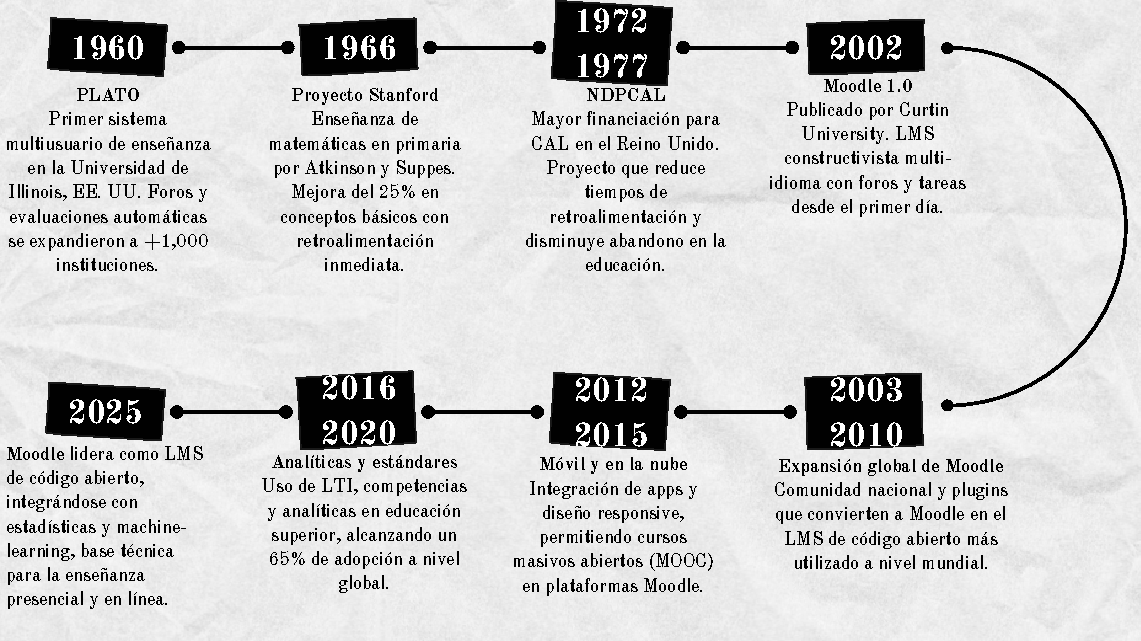
\includegraphics[width=1\textwidth]{Figs/Linea del Tiempo.pdf}
	\label{fig:LineaTiempo}
	\\Fuente: Elaboración propia con base en fuentes históricas.
\end{figure}

\subsection{Plataformas de aprendizaje}
Las plataformas de gestión del aprendizaje (LMS) como Moodle han revolucionado la educación digital desde su implementación. El caso pionero de la Universidad de Curtin en Australia en 2002 demostró que la adopción de Moodle en cursos de estadística descriptiva resultó en una mejora significativa en la participación estudiantil y una reducción del 30\% en los índices de reprobación, atribuible a la organización modular de contenidos y el acceso asíncrono a materiales \parencite{Pacheco2025}. Este tipo de resultados se alinea con el ciclo de validación continua que suele seguirse en la implementación de un LMS, como se resume en la Figura~\ref{fig:LMS}, donde se observa cómo la revisión iterativa de requisitos, contenidos y pruebas permite alcanzar un entorno de aprendizaje funcional y adaptado al contexto institucional.

\begin{figure}[ht]
    \centering
    \captionof{figure}{ \\ \vspace{0.5cm} Estado del arte. \textbf{Plataformas de aprendizaje}.}
    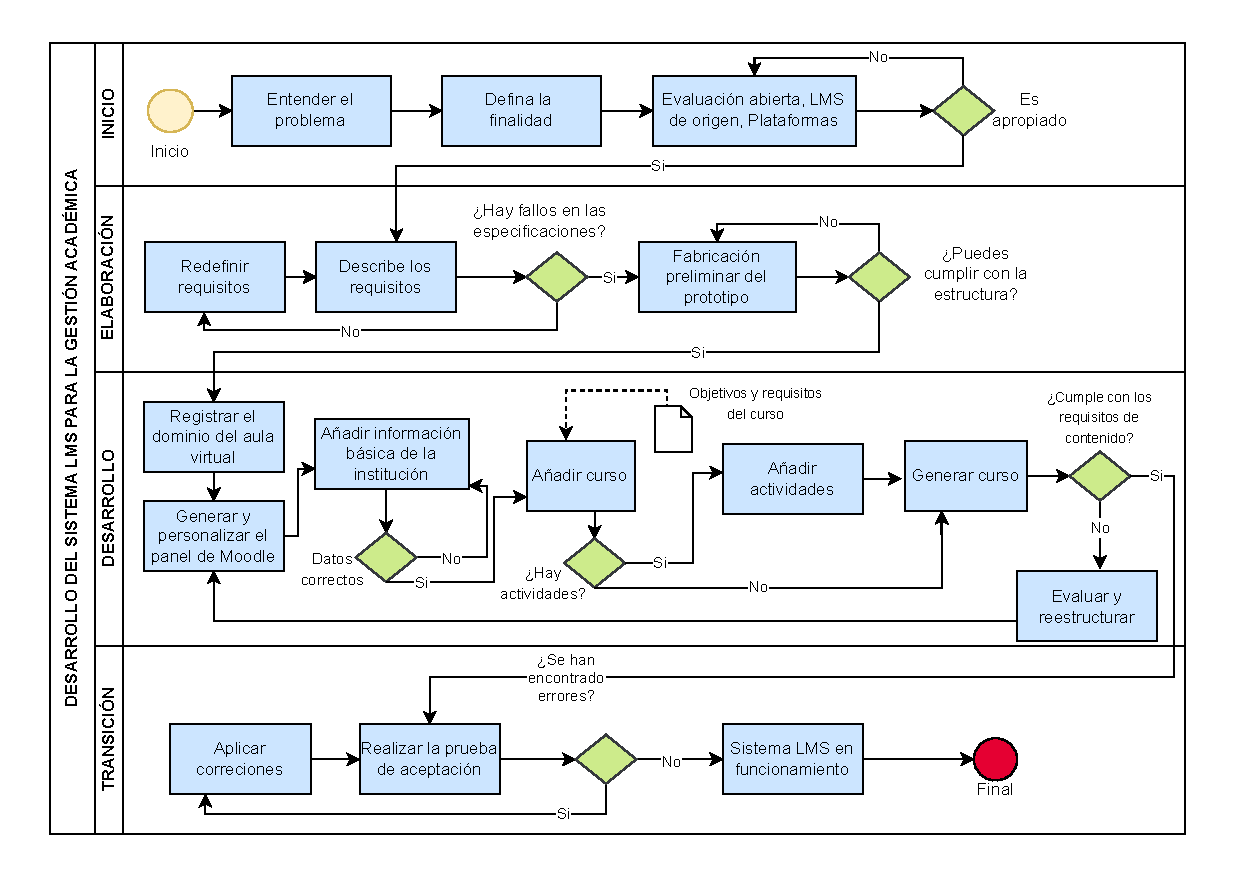
\includegraphics[width=0.8\textwidth]{Figs/LMS.pdf}
    \label{fig:LMS}
    \\Fuente: Adaptada de \textcite{Pacheco2025}
\end{figure}

Más recientemente, en 2025, la Universidad Nacional de Educación a Distancia (UNED) de España desarrolló un MOOC de estadística en Moodle que alcanzó una tasa de finalización del 68\%, superior al promedio de cursos masivos. Este éxito se atribuyó al uso de evaluaciones automáticas, foros moderados y contenido multimedia adaptativo. En contextos de menores recursos, la Universidad Pública de El Alto en Bolivia implementó Moodle para Estadística II en 2024, logrando mejoras significativas en la claridad de contenidos y el rendimiento académico de los estudiantes \parencite{Ndibalema2025}.

Estos ejemplos demuestran que Moodle no solo cumple funciones administrativas, sino que puede ser una fuente valiosa de información para mejorar la enseñanza de la estadística cuando se complementa con herramientas externas de análisis y práctica computacional. Las analíticas de aprendizaje basadas en el uso del LMS se han convertido en un campo emergente, donde la persistencia y constancia de los estudiantes en el uso de la plataforma se correlaciona directamente con el éxito académico, abriendo la puerta a modelos predictivos de intervención temprana \parencite{Goh2025}.

\subsection{Sistemas de Autoevaluación y Retroalimentación Automatizada}
La retroalimentación inmediata es crucial en la consolidación del aprendizaje estadístico. Mientras que los entornos tradicionales se centran en respuestas cerradas, las herramientas modernas han expandido su alcance hacia problemas complejos. El proyecto \textit{nbgrader}, implementado en la Universidad de Berkeley en 2017, permitió evaluar automáticamente tareas de estadística en Jupyter Notebooks, validando tanto la exactitud numérica como la lógica del código en Python, resultando en una reducción del 40\% en el tiempo de calificación y un aumento en la precisión de las evaluaciones \parencite{Blank2017}.

Sin embargo, investigaciones recientes identifican limitaciones persistentes. En 2024, la Universidad de Kuwait implementó un sistema de autoevaluación en estadística inferencial que, aunque efectivo para respuestas numéricas, no pudo evaluar el razonamiento estadístico ni la justificación de procedimientos, evidenciando la necesidad de graders más avanzados que trasciendan la simple comparación de valores \parencite{AlHaddad2024}.

Estas limitaciones subrayan la importancia de desarrollar sistemas de evaluación más sofisticados. Diversos estudios han sugerido que una alternativa futura es integrar graders más avanzados que almacenen y auditen código, permitiendo no solo verificar respuestas correctas o incorrectas, sino también analizar el proceso de resolución seguido por el estudiante, aumentando la transparencia y equidad en la evaluación.


\subsection{Arquitectura tecnológica para la educación}

En el ámbito de la enseñanza de la estadística, la discusión sobre arquitecturas tecnológicas ha pasado de enfocarse en plataformas de gestión administrativa hacia propuestas que buscan integrar entornos de análisis, retroalimentación inmediata y evaluación automatizada \parencite{Blank2017}, como se puede ver presente en la Figura~\ref{fig:architecture_E-learning}. Moodle continúa siendo una referencia obligada en la educación digital, especialmente por su capacidad para organizar contenidos y actividades. Sin embargo, varios estudios coinciden en que, aunque resulta eficaz para estructurar cursos, no responde por completo a las exigencias de la enseñanza de la estadística inferencial, en la que interesa no solo el resultado final, sino también el razonamiento seguido por el estudiante \parencite{Pacheco2025, Ndibalema2025}.

\begin{figure}[ht]
    \centering
    \captionof{figure}{ \\ \vspace{0.5cm} Estado del arte. \textbf{Arquitectura tecnológica para la educación}.}
    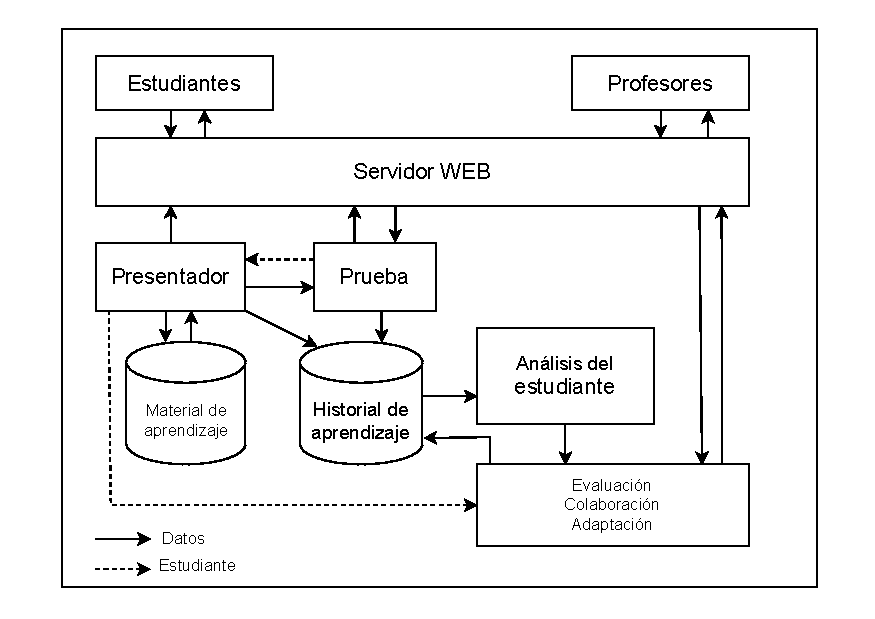
\includegraphics[width=0.9\textwidth]{Figs/Arquitectura_E-learning.pdf}
    \label{fig:architecture_E-learning}
    \\Fuente: Adaptada de \textcite{Mostefai2025}
\end{figure}


Ante esta limitación, algunas instituciones han apostado por combinar los LMS con entornos de programación y análisis de datos. Un ejemplo temprano es JupyterHub con nbgrader, desarrollado en la Universidad de California, Berkeley, que se consolidó como un referente en cursos masivos de ciencia de datos al permitir la entrega, ejecución y calificación automática de notebooks de Python \parencite{berkeley2018}. Por otro lado, la Universidad de Auckland ha incorporado RStudio Cloud para facilitar la práctica con R en cursos de inferencia y análisis de datos, priorizando la accesibilidad en la web \parencite{rubio2023}. Finalmente, en Carnegie Mellon University se ha implementado Autolab, pensado para la calificación de código en línea con control de intentos y reportes de error detallados \parencite{rubio2023}.

El diseño de entornos educativos digitales exige arquitecturas escalables, flexibles y seguras. En 2025, Mostefai propuso una arquitectura de microservicios para plataformas educativas que separa la lógica de negocio, la visualización de resultados y la gestión de datos en componentes independientes se puede ver representado en la Figura~\ref{fig:Microservicios}. Esta arquitectura permitió escalar cursos de estadística con más de 5.000 estudiantes simultáneos sin pérdida de rendimiento, mejorando significativamente la mantenibilidad y escalabilidad de los sistemas \parencite{Mostefai2025}.

\begin{figure}[ht]
    \centering
    \captionof{figure}{ \\ \vspace{0.5cm} Estado del arte. \textbf{Arquitectura de microservicios}.}
    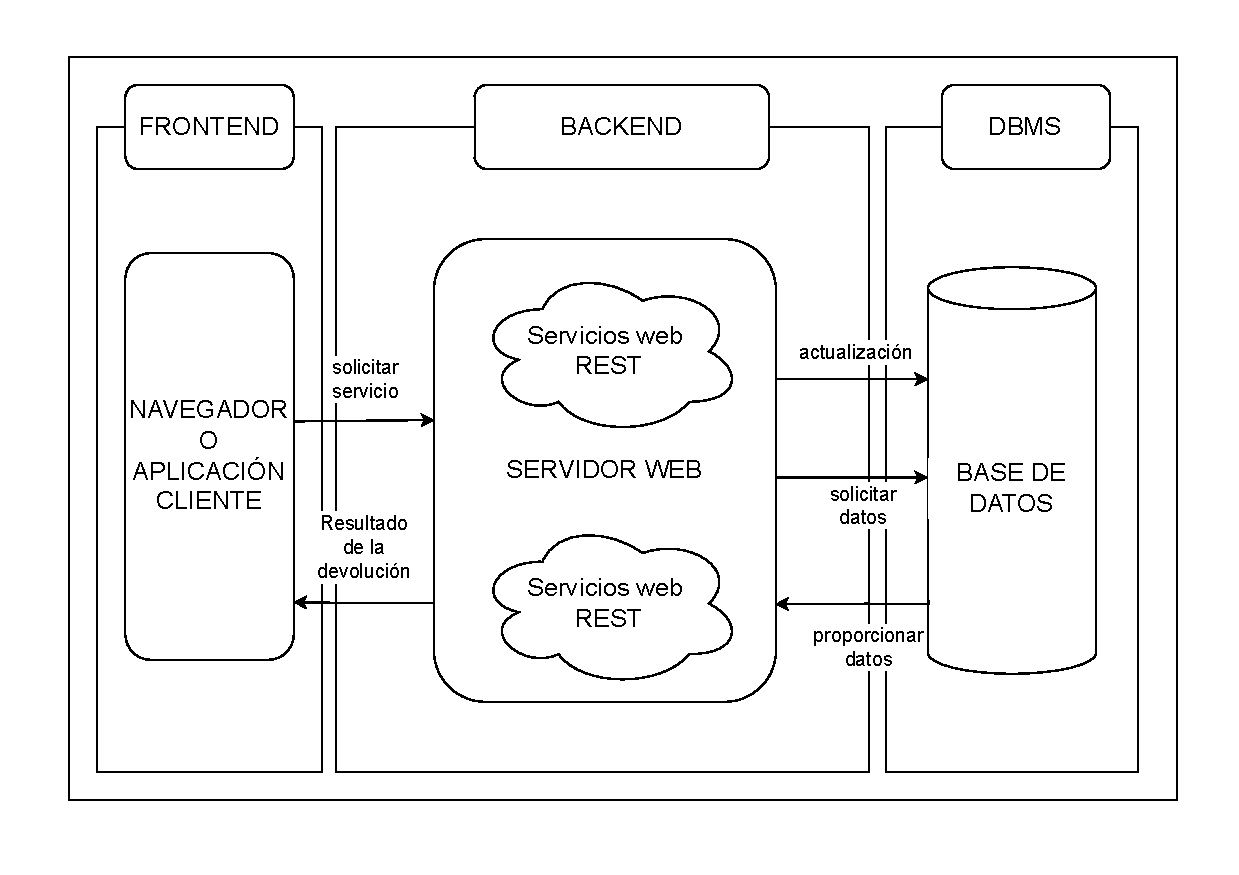
\includegraphics[width=0.9\textwidth]{Figs/Microservicios.pdf}
    \label{fig:Microservicios}
    \\Fuente: Adaptada de \textcite{Mostefai2025}
\end{figure}



Estas experiencias muestran un avance real hacia la automatización de la evaluación y la integración con el aprendizaje activo. Sin embargo, también dejan en evidencia limitaciones importantes. Por un lado, dependen de infraestructura institucional robusta o de licencias de pago, lo que restringe su uso en contextos de menor presupuesto. Además, suelen enfocarse en verificar la exactitud del código o los resultados numéricos, pero no siempre logran capturar la trazabilidad del razonamiento estadístico, que es clave en la formación en inferencia \parencite{alhaddad2024}.



\subsection{Antecedentes nacionales y la UIS}

En el contexto colombiano, la Universidad Industrial de Santander (UIS) ha sido pionera en el 
desarrollo de iniciativas que fortalecen la enseñanza y el aprendizaje de la estadística, 
articulando recursos digitales, programas de formación y unidades de análisis institucional. 
Desde mediados de la década de 2010, el Grupo SIMON de la UIS diseñó el software Evolución, una 
herramienta de modelado y simulación con dinámica de sistemas utilizada como apoyo en procesos 
formativos y de investigación, lo que refleja una apuesta temprana por el uso de simuladores en 
la enseñanza de disciplinas cuantitativas \parencite{simon2016}.

De manera complementaria, la Dirección de Nuevas Tecnologías de la Información y las Comunicaciones
 (NTIC) de la UIS consolidó un repositorio de software y simuladores disponibles para estudiantes 
 y docentes, los cuales abarcan desde áreas de ingeniería hasta aplicaciones estadísticas, 
 contribuyendo al fortalecimiento del aprendizaje autónomo y práctico \parencite{nticsf}. Esta 
 apuesta tecnológica se ha acompañado de la creación de la Unidad de Información y Análisis 
 Estadístico (UIAES), orientada a centralizar datos institucionales y a promover el uso de la 
 estadística como herramienta de apoyo en la gestión académica y administrativa, lo que evidencia
  una integración de la estadística no solo en la docencia, sino también en la toma de decisiones 
  estratégicas \parencite{uiassf}.

En el ámbito de la formación avanzada, la UIS ha ofrecido desde hace más de dos décadas la 
Especialización en Estadística, adscrita a la Escuela de Matemáticas. Este programa de posgrado 
se ha consolidado como referente nacional, orientando profesionales en el manejo de metodologías 
estadísticas aplicadas en contextos empresariales, educativos y de investigación 
\parencite{especializacionstatssf}. Estas iniciativas evidencian el papel de la UIS como 
institución líder en la innovación y consolidación de propuestas académicas que integran 
recursos digitales, analítica institucional y programas de formación especializada.

En la Universidad Industrial de Santander (UIS), el Centro de Experiencias y 
Tecnologías de Información y Comunicación \textit{EXPERTIC} se ha consolidado como un actor clave 
en la incorporación de TIC para fortalecer la docencia, la investigación y la extensión universitaria. 
Este centro promueve la innovación educativa mediante el diseño de recursos digitales, la gestión de 
plataformas tecnológicas y el acompañamiento a docentes y estudiantes en el uso pedagógico de las 
herramientas digitales \parencite{UIS2025a}. 

A nivel nacional, otras universidades también han contribuido a la consolidación de la estadística
 como disciplina clave para la educación superior y la investigación aplicada. Por ejemplo, la 
 Universidad Católica de Pereira desarrolló un módulo didáctico para el manejo estadístico de 
 datos en laboratorios de Física, destacando la transversalidad de la estadística en diferentes 
 campos del conocimiento \parencite{ucp2018}. Por su parte, la Fundación Universitaria Los 
 Libertadores ofrece la Especialización en Estadística Aplicada en modalidad virtual, ampliando 
 el acceso a formación especializada y evidenciando el interés creciente por programas flexibles 
 que integren la estadística con entornos digitales \parencite{libertadoressf}.

En este contexto, el presente trabajo de grado se inscribe como un aporte innovador al 
integrar en la asignatura de \textit{Estadística II} de la UIS un ambiente virtual de aprendizaje 
que combina \textit{Moodle} con entornos de programación (\textit{Python} y \textit{R}), 
\textit{Google Colab}, evaluadores automáticos (\textit{graders}) y arquitecturas de despliegue en 
\textit{Docker}. La propuesta busca responder a las limitaciones señaladas en la literatura, 
especialmente la ausencia de retroalimentación inmediata. Para ello, se plantea un entorno que 
incorpora actividades interactivas, mecanismos de autoevaluación y un plan de aula estructurado, 
implementado en dos grupos. De esta manera, el proyecto no solo fortalece la enseñanza de la 
estadística inferencial en pregrado, sino que se alinea con las tendencias internacionales de 
integración entre LMS.

\newpage

\chapter{Metodología}

La metodología empleada en este proyecto se diseñó con el propósito de articular de manera efectiva los componentes tecnológicos, pedagógicos y organizativos que hicieron posible el desarrollo del ambiente de aprendizaje para la enseñanza de Estadística II. Se adoptó un enfoque ágil \textit{Scrum}, que estructuro el trabajo en ciclos cortos de planificación, desarrollo y evaluación, denominados \textit{sprints}. Esta elección metodológica favoreció una gestión ordenada de las tareas, una comunicación constante entre los participantes y la incorporación progresiva de nuevas funcionalidades, manteniendo siempre el enfoque en los objetivos académicos del proyecto.

Se presentan las estrategias y procedimientos utilizados para llevar a cabo cada fase del proceso de desarrollo. Se describen los roles asumidos por el equipo, la organización del trabajo mediante \textit{sprints} y las herramientas tecnológicas que facilitaron la implementación, como la arquitectura de microservicios basada en \textit{Node.js}, \textit{React}, \textit{MariaDB} y \textit{Docker}, así como soluciones complementarias como \textit{Playit.gg} y \textit{Safe Exam Browser}. Esta estructura metodológica permitió avanzar de forma controlada y flexible, garantizando que cada entrega parcial fortaleciera la integración entre los contenidos académicos y las funciones esperadas para la autoevaluación de los \textit{graders}.


\section{Enfoque metodológico}

Para el desarrollo del presente proyecto se adoptó la metodología ágil Scrum, debido a que permitió organizar el trabajo en iteraciones cortas (sprints), promover la retroalimentación constante y garantizar la entrega continua de productos funcionales. Este enfoque se ajustó a la naturaleza del proyecto, en el cual se requirió diseñar, implementar y validar materiales interactivos y evaluativos para la asignatura Estadística II en un ambiente de aprendizaje.

Según \cite{schwaber2013scrum}, ``Scrum es un marco de trabajo por el cual las personas pueden acometer problemas complejos adaptativos, a la vez que entregar productos del máximo valor posible productiva y creativamente''.

\section{Pasos generales de la metodología}

La metodología del proyecto se estructuró en función de los objetivos específicos, los cuales se materializaron en una serie de acciones interrelacionadas.

En primer lugar, para el diseño de un plan de aula modular, se realizó una revisión y selección de los contenidos teóricos y prácticos más relevantes de la asignatura, en conjunto con los docentes responsables (Anexo \ref{anexo:acta-abril-2025}). Posteriormente, estos contenidos fueron organizados en unidades interactivas implementadas en Colab Notebooks con Python y R, incorporando actividades prácticas y calificadores automáticos que ofrecieron retroalimentación inmediata.

En cuanto a la implementación del ambiente virtual de aprendizaje en Moodle, se inició con la configuración de la estructura del curso, organizando por semanas con el fin de mantener un orden y control de los contenidos. A continuación, se integraron los Colab Notebooks, los materiales didácticos de apoyo y diversos recursos multimedia que fortalecieron la experiencia pedagógica. Finalmente, se llevaron a cabo pruebas de funcionamiento tanto técnico como pedagógico, con el propósito de verificar la accesibilidad y coherencia de los recursos integrados.

Para el establecimiento de los instrumentos de medición, se diseñaron actividades evaluativas en Moodle basadas en los calificadores automáticos, definiendo indicadores específicos para valorar el logro de los resultados de aprendizaje. Estos instrumentos fueron implementados de manera piloto y ajustados a partir de la retroalimentación proporcionada por los docentes, lo cual permitió afinar su pertinencia y validez.

Finalmente, con el objetivo de pilotear el ambiente de aprendizaje diseñado, se seleccionaron dos grupos de la asignatura Estadística II y se coordinó con los docentes responsables para aplicar el plan de aula y los instrumentos de evaluación. El proceso de pilotaje incluyó la recolección de datos sobre la usabilidad de la herramienta, la satisfacción de los estudiantes y la efectividad en términos de resultados de aprendizaje.

En conjunto, estos pasos establecieron una relación directa entre los objetivos y las actividades realizadas, garantizando que cada etapa metodológica aportara al cumplimiento integral del proyecto.

\section{Roles}

El equipo estuvo conformado por tres integrantes: un docente y dos practicantes (los autores del presente proyecto).

\subsection*{Scrum Master (Docente)}
\begin{itemize}[leftmargin=*]
	\item Definir los temas a desarrollar en cada iteración.
	\item Validar los entregables (material teórico, graders y servidor de calificaciones).
	\item Proporcionar retroalimentación y ajustes necesarios.
\end{itemize}

\subsection*{Desarrolladores (Practicantes)}
Encargados de distribuirse las tareas correspondientes a cada sprint, las cuales incluyeron:
\begin{itemize}[leftmargin=*]
	\item Elaborar el material teórico, diseñado para integrarse en Moodle y con un enfoque interactivo.
	\item Diseñar e implementar los graders (evaluadores automáticos) para los ejercicios prácticos.
	\item Programar la lógica del servidor que permitió calificar y almacenar los resultados.
	\item Ejecutar las correcciones solicitadas por el Scrum Master.
\end{itemize}

\section{Estructura de los sprints}

El proyecto se organizó en sprints semanales, cada uno correspondiente al diseño y validación de una práctica de la asignatura. En total se llevaron a cabo nueve sprints, alineados con las ocho prácticas definidas en el curso de Estadística II y contando con 2 cuestionarios. La dinámica de trabajo semanal fue la siguiente:

\begin{itemize}
	\item \textbf{Sábado:} el Scrum Master definió los temas correspondientes a la semana.  
	\item \textbf{Miércoles (fecha límite):} los practicantes entregaron el material teórico, los graders y la versión funcional del servidor de calificaciones.  
	\item \textbf{Jueves:} el Scrum Master revisó los entregables y dio su aprobación o indicó las modificaciones requeridas.  
	\item \textbf{Viernes:} se liberaron los graders para que los estudiantes (grupo piloto) realizaran las prácticas.  
\end{itemize}

\section{Sprints}

\subsection{Sprint 0}

Este sprint se definió a partir de la reunión llevada a cabo el 2 de abril de 2025 en la sala de juntas de la Escuela de Ingeniería de Sistemas de la UIS. Los participantes fueron:

\begin{itemize}
	\item \textbf{Practicantes:} Daniel Alejandro Sánchez Rodríguez y Jorge Eduardo Suárez Cortés.
	\item \textbf{Profesores del área de Estadística II:} César Augusto Aceros Moreno, Eliana Martha Bonalde Marcano, Andrés Leonardo González Gómez, David Edmundo Romo Bucheli.
	\item \textbf{Dirección del proyecto en su fase inicial:} Sonia Cristina Gamboa Sarmiento.
\end{itemize}

\noindent Para mayor detalle de la reunión puede consultarse el acta correspondiente en el Anexo \ref{anexo:acta-abril-2025}.

En dicha reunión se establecieron los lineamientos iniciales del proyecto y se delimitó su alcance, acordando que el enfoque debía orientarse a mejorar los procesos de enseñanza y aprendizaje mediante el uso de herramientas digitales.  

Durante las discusiones se resaltó la importancia de analizar las características de los principales lenguajes de programación utilizados en el ámbito estadístico (Python, MATLAB y R). Con este propósito se propuso elaborar un cuadro comparativo que permitiera identificar sus ventajas, desventajas y entornos de desarrollo asociados. Aunque no se seleccionó un lenguaje específico en esta etapa, se dejó abierta la posibilidad de trabajar con más de uno, con el objetivo de garantizar flexibilidad.  

Asimismo, se planteó que la herramienta a desarrollar debía ser agnóstica respecto al lenguaje de programación, de modo que el usuario pudiera elegir libremente el entorno de su preferencia. También se discutió la conveniencia de incorporar interfaces visuales y elementos gráficos que fortalecieran la enseñanza para los estudiantes, junto con la organización de los contenidos pedagógicos dentro de Moodle como plataforma de apoyo.  

De manera complementaria, se estableció una distribución preliminar de temas en tres unidades (1.3 y 1.4; 2.3 y 2.4; 3.3 y 3.4), para estructurar las prácticas, realizar pruebas efectivas y evaluar el funcionamiento del proyecto.  

Finalmente, en este sprint se tomaron decisiones relacionadas con las tecnologías base que guiaron el desarrollo:  

\begin{itemize}
	\item \textbf{Node.js}: para el backend, debido a su rapidez en las respuestas y su estructura escalable.  
	\item \textbf{Moodle}: como plataforma para la gestión del contenido teórico.  
	\item \textbf{Google Colab}: como entorno de ejecución de los \textit{graders}, aprovechando su accesibilidad y la posibilidad de alternar entre los \textit{kernels} de Python y R.  
	\item \textbf{Docker}: para asegurar un despliegue estable y controlado mediante contenedores.  
	\item \textbf{Playit.gg}: como servicio de túnel que permitió exponer el servidor de calificaciones en internet.  
\end{itemize}

\subsection{Sprint 1}

\subsubsection*{Objetivos del Scrum Master (docente)}
\begin{itemize}
	\item Definir los temas a trabajar durante el sprint: medidas de tendencia central (media, mediana, moda), medidas de dispersión (rango, desviación estándar, varianza), histogramas y diagramas de caja (boxplots).
	\item Validar la pertinencia y calidad de los contenidos teóricos elaborados por los practicantes.
	\item Revisar el funcionamiento de los graders y su integración con el servidor de calificaciones.
	\item Orientar la definición de la arquitectura técnica, verificando que cumpliera con los lineamientos de escalabilidad y modularidad.
\end{itemize}

\subsubsection*{Cronograma del Sprint}
\begin{itemize}
	\item \textbf{Inicio del Sprint:} 9 de agosto de 2025 → El Scrum Master definió los temas a desarrollar.
	\item \textbf{Entrega de los practicantes:} 13 de agosto de 2025 → Se entregaron el material teórico en H5P, los graders y la estructura técnica inicial.
	\item \textbf{Revisión del Scrum Master:} 14 de agosto de 2025 → El material desarrollado por los practicantes no requirió modificaciones.
	\item \textbf{Liberación de recursos:} 15 de agosto de 2025 → Los graders y materiales teóricos fueron liberados en Moodle y Colab para ser utilizados por los grupos pilotos.
\end{itemize}

\subsubsection*{Actividades realizadas por los practicantes}

\begin{enumerate}
	\item \textbf{Estructura técnica del proyecto}
	\begin{itemize}
		\item Se definió el esqueleto del sistema, estableciendo la organización de los módulos (frontend, backend y grader).
		\item Se configuró la exposición de servicios y la comunicación entre módulos.
		\item Se organizó el sistema en contenedores con Docker, garantizando un entorno estable, replicable y modular.
	\end{itemize}
	
	\noindent Lo anterior se representó gráficamente en el esquema de los contenedores Docker mostrado en la Figura~\ref{fig:Diagrama-Docker}.
	
	\begin{figure}[ht]
		\centering
		\captionof{figure}{ \\ \vspace{0.5cm} Sprint 1. \textbf{Esquema de los contenedores Docker}.}
		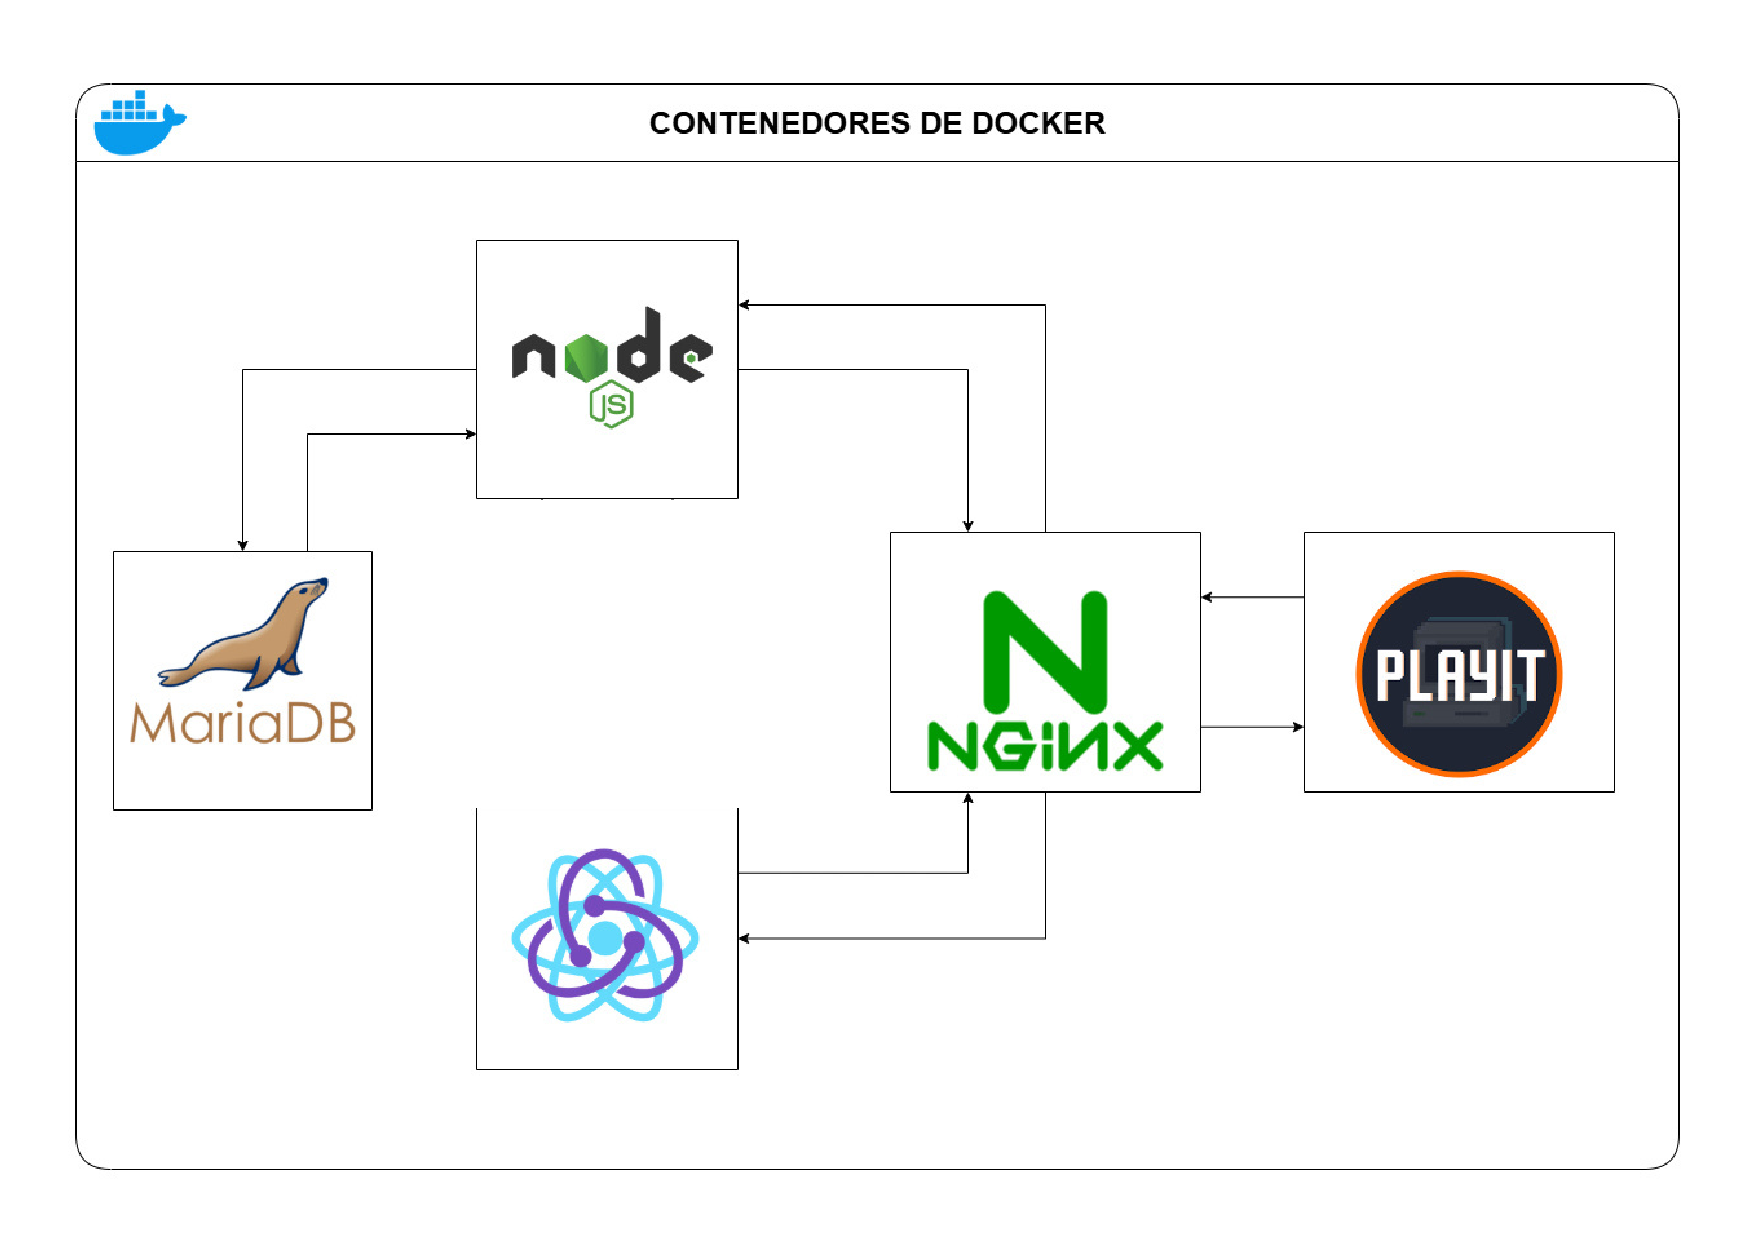
\includegraphics[width=0.8\textwidth]{Figs/Diagrama_contenedores.pdf}
		\label{fig:Diagrama-Docker}
		\\Fuente: Elaboración propia con base en la estructura de los contenedores usados.
	\end{figure}

	\item \textbf{Material teórico en Moodle}
	\begin{itemize}
		\item Se elaboraron recursos interactivos utilizando H5P dentro de Moodle.
		\item Los materiales incluyeron infografías sintetizadas con la información esencial para el aprendizaje de los temas, permitiendo una mayor comprensión visual.
		\item La construcción de los contenidos se fundamentó en los textos de referencia de \textcite{montgomery1996} y \textcite{walpole2012probabilidad}, autores reconocidos en estadística.
	\end{itemize}
	
	\item \textbf{Graders en Google Colab}
	\begin{itemize}
		\item Se desarrollaron notebooks en Google Colab utilizando código en R.
		\item Estos graders permitieron calcular medidas de tendencia central y dispersión, así como generar representaciones gráficas (histogramas y diagramas de caja).
	\end{itemize}
	
	\item \textbf{Ejercicios calificables y lógica en el backend}
	\begin{itemize}
		\item Se diseñaron tres ejercicios evaluables relacionados con los temas del sprint.
		\item Se implementó la lógica de corrección en el backend (Node.js) para procesar automáticamente las respuestas.
		\item El servidor de calificaciones registró y almacenó los resultados, garantizando un flujo de evaluación automatizado.
	\end{itemize}
\end{enumerate}

\subsection{Sprint 2}

\subsubsection*{Objetivos del Scrum Master (docente)}
\begin{itemize}
	\item Definir los temas estadísticos a abordar: Teorema del Límite Central aplicado a la distribución t-Student y la distribución F.
	\item Supervisar la ampliación de los recursos teóricos y prácticos, asegurando la coherencia pedagógica con el programa de la asignatura.
	\item Validar la correcta implementación de los graders y su funcionamiento.
	\item Orientar la mejora del frontend para optimizar la visualización de las calificaciones.
\end{itemize}

\subsubsection*{Cronograma del Sprint}
\begin{itemize}
	\item \textbf{Inicio del Sprint:} 16 de agosto de 2025 → Se definieron los temas estadísticos y se establecieron las prioridades técnicas.
	\item \textbf{Entrega de los practicantes:} 20 de agosto de 2025 → Se presentaron los nuevos materiales teóricos, graders funcionales y las primeras mejoras en la interfaz.
	\item \textbf{Revisión del Scrum Master:} 21 de agosto de 2025 → Se realizaron recomendaciones para mejorar la claridad de la usabilidad de los graders.
	\item \textbf{Liberación de recursos:} 22 de agosto de 2025 → Los graders y materiales teóricos fueron liberados en Moodle y Colab para ser utilizados por los grupos pilotos.
\end{itemize}

\subsubsection*{Actividades realizadas por los practicantes}

\begin{enumerate}
	\item \textbf{Ampliación de contenidos teóricos}  
	\begin{itemize}
		\item Se elaboraron materiales interactivos centrados en el Teorema del Límite Central y su aplicación con distribuciones t-Student y F, integrando teoría, ejemplos resueltos y gráficos interactivos.
		\item Se enfatizó en la interpretación de regiones de rechazo y grados de libertad, para reforzar el razonamiento inferencial de los estudiantes.
	\end{itemize}
	
	\item \textbf{Graders de distribuciones t y F en Google Colab}  
	\begin{itemize}
		\item Se desarrollaron nuevos notebooks en Google Colab utilizando código en R, enfocados en ejercicios prácticos sobre pruebas t y F.
		\item Los graders permitieron a los estudiantes realizar cálculos de valores críticos, regiones de rechazo y decisiones de hipótesis de forma automática.
	\end{itemize}
	
	\item \textbf{Ejercicios calificables y lógica en el backend}  
	\begin{itemize}
		\item Se diseñaron ejercicios evaluables sobre aplicaciones del Teorema del Límite Central con la distribución t y F, con distintos grados de dificultad.
		\item Se ajustaron los endpoints para almacenar no solo la nota final, sino también los códigos hechos por los estudiantes.
	\end{itemize}
	
	\item \textbf{Mejoras en el \textit{frontend} para visualización de calificaciones}  
	\begin{itemize}
		\item Se rediseñaron los componentes de interfaz relacionados con la visualización de notas y codigo de los estudiantes.
	\end{itemize}
\end{enumerate}

\subsection{Sprint 3}

\subsubsection*{Objetivos del Scrum Master (docente)}
\begin{itemize}
	\item Definir los contenidos estadísticos relacionados con intervalos de confianza, incluyendo sus diferentes tipos y aplicaciones prácticas.
	\item Supervisar la elaboración de recursos teóricos y ejercicios prácticos que permitan comprender la construcción e interpretación de intervalos.
	\item Validar el funcionamiento de los graders desarrollados para cálculos de intervalos de confianza, de predicción y de tolerancia.
\end{itemize}

\subsubsection*{Cronograma del Sprint}
\begin{itemize}
	\item \textbf{Inicio del Sprint:} 23 de agosto de 2025 → Se establecieron los temas estadísticos, los entregables técnicos y pedagógicos, y las prioridades de desarrollo.
	\item \textbf{Entrega de los practicantes:} 27 de agosto de 2025 → Se presentaron los materiales teóricos, graders implementados y los ejercicios evaluables.
	\item \textbf{Revisión del Scrum Master:} 28 de agosto de 2025 → Se realizaron observaciones sobre el material teórico.
	\item \textbf{Liberación de recursos:} 29 de agosto de 2025 → Se publicaron los recursos validados en Moodle y Colab para ser utilizados en el entorno piloto.
\end{itemize}

\subsubsection*{Actividades realizadas por los practicantes}

\begin{enumerate}
	\item \textbf{Desarrollo de contenidos teóricos sobre intervalos}  
	\begin{itemize}
		\item Se elaboraron materiales interactivos en genially que abordaron los fundamentos de los intervalos de confianza y sus aplicaciones.
		\item Se diferenciaron claramente los intervalos bilaterales y unilaterales, explicando su uso en distintos contextos inferenciales.
		\item Se incluyeron ejemplos prácticos sobre intervalos con varianza conocida y desconocida, así como intervalos de predicción e intervalos de tolerancia.
	\end{itemize}
	
	\item \textbf{Graders para intervalos en Google Colab}  
	\begin{itemize}
		\item Se diseñaron notebooks en Google Colab contando con diferentes ejercicios para cada grupo piloto.
		\item Los graders permitieron a los estudiantes ingresar datos muestrales y obtener intervalos de confianza, predicción y tolerancia.
	\end{itemize}
	
	\item \textbf{Ejercicios calificables y lógica en el backend}  
	\begin{itemize}
		\item Se desarrollaron ejercicios evaluables enfocados en la construcción e interpretación de distintos tipos de intervalos.
		\item Se amplió la lógica del backend para manejar escenarios con diferentes tipos de error, distinguiendo entre errores de cálculo, interpretación y selección de tipo de intervalo.
	\end{itemize}
	
\end{enumerate}

\subsection{Sprint 4}

\subsubsection*{Objetivos del Scrum Master (docente)}
\begin{itemize}
	\item Definir los contenidos y lineamientos técnicos para la implementación manual del método bootstrap en Python.
	\item Supervisar la creación de materiales teóricos y prácticos que expliquen el cálculo del error estándar (SE), sesgo (\textit{bias}) e intervalos de confianza con bootstrap.
	\item Validar la correcta ejecución de los algoritmos de remuestreo y su integración en los graders desarrollados por los practicantes.
	\item Orientar la estructuración de ejercicios prácticos que fortalezcan la comprensión conceptual y computacional del método bootstrap.
\end{itemize}

\subsubsection*{Cronograma del Sprint}
\begin{itemize}
	\item \textbf{Inicio del Sprint:} 30 de agosto de 2025 → Se definieron los objetivos conceptuales y técnicos del sprint, priorizando la correcta implementación manual del bootstrap.
	\item \textbf{Entrega de los practicantes:} 3 de septiembre de 2025 → Se entregaron los materiales teóricos, notebooks en Python y ejercicios evaluables asociados.
	\item \textbf{Revisión del Scrum Master:} 4 de septiembre de 2025 → Se revisó la precisión de los algoritmos de remuestreo y la claridad pedagógica de los contenidos.
	\item \textbf{Liberación de recursos:} 5 de septiembre de 2025 → Se publicaron los recursos validados en Moodle y Colab, quedando listos para ser utilizados por los grupos pilotos.
\end{itemize}

\subsubsection*{Actividades realizadas por los practicantes}

\begin{enumerate}
	\item \textbf{Material teórico sobre el método bootstrap}  
	\begin{itemize}
		\item Se elaboraron recursos interactivos en genially que explicaron la teoria del remuestreo bootstrap.
		\item Se incluyeron secciones dedicadas al cálculo manual del error estándar, el sesgo y los intervalos de confianza bajo el enfoque bootstrap normal.
	\end{itemize}
	
	\item \textbf{Implementación manual de bootstrap en Python}  
	\begin{itemize}
		\item Se desarrollaron notebooks en Google Colab utilizando Python, implementando desde cero el algoritmo bootstrap sin librerías externas de alto nivel.
		\item Los scripts permitieron realizar múltiples remuestreos, calcular el error estándar, el sesgo y construir intervalos de confianza normales.
	\end{itemize}
	
	\item \textbf{Graders y ejercicios evaluables}  
	\begin{itemize}
		\item Se diseñaron ejercicios calificables que exigían aplicar el método bootstrap manualmente para estimar parámetros y sus intervalos de confianza.
		\item La lógica del backend fue adaptada para validar los resultados por parte de los estudiantes.
	\end{itemize}
	
\end{enumerate}

\subsection{Sprint 5}

\subsubsection*{Objetivos del Scrum Master (docente)}
\begin{itemize}
	\item Diseñar y supervisar la preparación de una evaluación tipo \textit{cuestionario} para medir la apropiación de los conceptos estadísticos y computacionales desarrollados en los sprints anteriores.
	\item Garantizar que la estructura del cuestionario combine tanto la aplicación práctica de métodos de bootstrap como la comprensión teórica de intervalos y distribuciones.
	\item Validar la correcta configuración técnica de Moodle y Safe Exam Browser para asegurar un entorno controlado y minimizar prácticas de deshonestidad académica.
\end{itemize}

\subsubsection*{Cronograma del Sprint}
\begin{itemize}
	\item \textbf{Inicio del Sprint:} 6 de septiembre de 2025 → Se definieron la estructura del cuestionario, los temas a evaluar y la estrategia técnica para su implementación.
	\item \textbf{Entrega de los practicantes:} 10 de septiembre de 2025 → Se presentaron las preguntas, ejercicios y configuraciones en Moodle.
	\item \textbf{Revisión del Scrum Master:} 11 de septiembre de 2025 → Se revisó la claridad conceptual de las preguntas, la adecuación de la dificultad y la correcta configuración de la plataforma.
	\item \textbf{Liberación de recursos:} 12 de septiembre de 2025 → Se aprobó la versión final del cuestionario y se habilitó en el entorno de Moodle, listo para su aplicación controlada.
\end{itemize}

\subsubsection*{Actividades realizadas por los practicantes}

\begin{enumerate}
	\item \textbf{Diseño de la estructura general del cuestionario}  
	\begin{itemize}
		\item Se definió un cuestionario con duración total de dos horas, dividido en dos partes: una práctica presencial y una teórica en Moodle.
		\item La evaluación se planificó para cubrir tanto competencias de cálculo manual con bootstrap, como la comprensión teórica de conceptos clave de inferencia estadística.
	\end{itemize}
	
	\item \textbf{Primera parte: Ejercicios de bootstrap en RStudio}  
	\begin{itemize}
		\item Se diseñaron dos ejercicios prácticos que debían resolverse manualmente en RStudio sin acceso a internet.
		\item En cada ejercicio, los estudiantes debían calcular la \textbf{mediana}, el \textbf{sesgo (bias)}, el \textbf{error estándar (SE)}, la \textbf{asimetría (skewness)} y el \textbf{intervalo de confianza} (determinando si corresponde usar el método normal o percentil).
		\item Los resultados finales se consignaron en una hoja de respuestas física, que fue recolectada al finalizar esta primera parte.
		\item Esta sección buscó evaluar la capacidad de los estudiantes para aplicar el método bootstrap manualmente y razonar sobre la elección del tipo de intervalo.
	\end{itemize}
	
	\item \textbf{Segunda parte: cuestionario en Moodle con Safe Exam Browser}  
	\begin{itemize}
		\item La segunda sección consistió en un cuestionario de cuatro preguntas teóricas seleccionadas aleatoriamente por Moodle de un banco de ejercicios previamente preparados.
		\item Los temas abordados fueron:
		\begin{itemize}
			\item Intervalos de confianza.
			\item Intervalos de tolerancia.
			\item Distribuciones de muestreo de medias y Teorema del Límite Central.
			\item Estadísticas importantes: medidas de tendencia central y de variabilidad de la muestra.
			\item Estimación de la varianza en muestra única.
			\item Intervalos de predicción.
		\end{itemize}
		\item Para esta parte, se configuró el uso obligatorio de \textit{Safe Exam Browser}, una herramienta que permite controlar el entorno del examen y reducir significativamente la posibilidad de trampas académicas.
		\item La plataforma seleccionó las preguntas de manera aleatoria para cada estudiante, incrementando la equidad y la robustez de la evaluación.
	\end{itemize}
\end{enumerate}

\subsection{Sprint 6}

\subsubsection*{Objetivos del Scrum Master (docente)}
\begin{itemize}
	\item Definir los contenidos teóricos y prácticos relacionados con pruebas de hipótesis para una muestra en el contexto de distribuciones normales.
	\item Supervisar la elaboración de materiales pedagógicos que aborden los diferentes tipos de hipótesis (unilaterales y bilaterales) y los errores asociados (Tipo I y Tipo II).
	\item Validar el correcto diseño e implementación de los graders en Colab para ejercicios de pruebas de hipótesis, incluyendo el cálculo de potencia estadística (\textit{power}), error tipo II (\(\beta\)) y valores \textit{p}.
\end{itemize}

\subsubsection*{Cronograma del Sprint}
\begin{itemize}
	\item \textbf{Inicio del Sprint:} 13 de septiembre de 2025 → Se definieron los contenidos estadísticos y técnicos a desarrollar durante el sprint.
	\item \textbf{Entrega de los practicantes:} 17 de septiembre de 2025 → Se presentaron los materiales teóricos, notebooks interactivos y ejercicios evaluables.
	\item \textbf{Revisión del Scrum Master:} 18 de septiembre de 2025 → Se verificó la precisión conceptual y estadística de los materiales y graders.
	\item \textbf{Liberación de recursos:} 19 de septiembre de 2025 → Se publicaron los recursos en Moodle y Colab para su uso por los grupos pilotos.
\end{itemize}

\subsubsection*{Actividades realizadas por los practicantes}

\begin{enumerate}
	\item \textbf{Desarrollo de contenidos teóricos sobre pruebas de hipótesis}  
	\begin{itemize}
		\item Se elaboraron materiales interactivos en Genially que explican la teoría de una prueba de hipótesis para:
		\begin{enumerate}
			\item La media de una distribución normal con varianza conocida.
			\item La media de una distribución normal con varianza desconocida.
			\item La varianza y la desviación estándar de una distribución normal.
		\end{enumerate}
		\item Cada caso incluyó la identificación de hipótesis nula y alternativa, la selección adecuada del tipo de prueba (cola derecha, cola izquierda o bilateral), y la representación gráfica de la región de rechazo.
		\item Se incorporaron explicaciones conceptuales sobre el error tipo II (\(\beta\)), la potencia de la prueba (\(1 - \beta\)) y la interpretación del valor \textit{p}.
	\end{itemize}
	
	\item \textbf{Graders para pruebas de hipótesis en Google Colab}  
	\begin{itemize}
		\item Se desarrollaron notebooks en Google Colab utilizando Python para ejercicios prácticos relacionados con pruebas de hipótesis para una muestra.
		\item Los graders guiaron a los estudiantes en la identificación de parámetros poblacionales, formulación de hipótesis, determinación de regiones críticas y cálculo de estadísticos de prueba.
		\item Además, permitieron calcular el error tipo II, la potencia estadística y el valor \textit{p} asociado a cada prueba.
	\end{itemize}
	
	\item \textbf{Ejercicios evaluables y lógica en el backend}  
	\begin{itemize}
		\item Se diseñaron ejercicios calificables de diferentes niveles de dificultad, abarcando pruebas unilaterales y bilaterales.
		\item Se implementaron endpoints en el backend para procesar automáticamente las respuestas de los estudiantes y registrar sus resultados.
	\end{itemize}
\end{enumerate}

\subsection{Sprint 7}

\subsubsection*{Objetivos del Scrum Master (docente)}
\begin{itemize}
	\item Definir los contenidos teóricos y prácticos relacionados con \textbf{pruebas de hipótesis para dos muestras}, como continuación natural del Sprint 6 (hipótesis para una muestra).
	\item Supervisar la elaboración de materiales pedagógicos que aborden los diferentes escenarios de comparación de dos poblaciones, incluyendo casos con varianzas conocidas, varianzas desconocidas iguales y varianzas desconocidas distintas.
	\item Validar la correcta implementación de los graders en Google Colab para ejercicios de pruebas de hipótesis con dos muestras, incluyendo el cálculo de estadísticos de prueba, regiones de rechazo, valores \textit{p} y potencia estadística.
\end{itemize}

\subsubsection*{Cronograma del Sprint}
\begin{itemize}
	\item \textbf{Inicio del Sprint:} 20 de septiembre de 2025 → Se definieron los contenidos estadísticos y técnicos a desarrollar durante el sprint.
	\item \textbf{Entrega de los practicantes:} 24 de septiembre de 2025 → Se presentaron los materiales teóricos, notebooks interactivos y ejercicios evaluables.
	\item \textbf{Revisión del Scrum Master:} 25 de septiembre de 2025 → Se verificó la precisión conceptual y estadística de los materiales y graders.
	\item \textbf{Liberación de recursos:} 26 de septiembre de 2025 → Se publicaron los recursos en Moodle y Colab para su uso por los grupos pilotos.
\end{itemize}

\subsubsection*{Actividades realizadas por los practicantes}

\begin{enumerate}
	\item \textbf{Desarrollo de contenidos teóricos sobre pruebas de hipótesis para dos muestras}  
	\begin{itemize}
		\item Se elaboraron materiales interactivos en Genially que explican la teoría y procedimientos de pruebas de hipótesis para:
		\begin{enumerate}
			\item Comparación de medias de dos poblaciones con varianzas conocidas.
			\item Comparación de medias con varianzas desconocidas pero iguales.
			\item Comparación de medias con varianzas desconocidas y diferentes (prueba t de Welch).
		\end{enumerate}
		\item Se incluyeron explicaciones detalladas sobre la formulación de hipótesis nula y alternativa, la elección de pruebas unilaterales o bilaterales, y la representación gráfica de las regiones de rechazo correspondientes.
		\item Se abordaron conceptos de error Tipo I, error Tipo II y potencia estadística en el contexto de pruebas con dos muestras.
	\end{itemize}
	
	\item \textbf{Graders para pruebas de hipótesis con dos muestras en Google Colab}  
	\begin{itemize}
		\item Se desarrollaron notebooks interactivos en Google Colab utilizando Python para resolver ejercicios prácticos de comparación de dos muestras.
		\item Los graders guiaron a los estudiantes en la identificación de parámetros, formulación de hipótesis, selección del tipo de prueba adecuado (z o t), cálculo de estadísticos y toma de decisiones.
		\item Se implementaron funciones para el cálculo automático de valores \textit{p}, regiones críticas y potencia de la prueba bajo distintos escenarios.
	\end{itemize}
	
\end{enumerate}

\subsection{Sprint 8}

\subsubsection*{Objetivos del Scrum Master (docente)}
\begin{itemize}
	\item Introducir el método de \textbf{Monte Carlo} como una herramienta fundamental para la simulación y aproximación de resultados estadísticos mediante generación de números aleatorios.
	\item Supervisar el desarrollo de ejercicios prácticos que permitan a los estudiantes comprender la lógica detrás de la simulación Monte Carlo de forma manual, sin depender exclusivamente de librerías estadísticas avanzadas.
	\item Validar la correcta implementación de los notebooks en Google Colab para garantizar que los procedimientos y resultados obtenidos por simulación sean coherentes con la teoría estadística.
\end{itemize}

\subsubsection*{Cronograma del Sprint}
\begin{itemize}
	\item \textbf{Inicio del Sprint:} 27 de septiembre de 2025 → Se definieron los contenidos teóricos y prácticos relacionados con el método de Monte Carlo.
	\item \textbf{Entrega de los practicantes:} 1 de octubre de 2025 → Se entregaron los primeros notebooks con simulaciones manuales en Python y ejercicios guía.
	\item \textbf{Revisión del Scrum Master:} 2 de octubre de 2025 → Se revisó la claridad pedagógica, la corrección estadística de los procedimientos y la funcionalidad del código en Colab.
	\item \textbf{Liberación de recursos:} 3 de octubre de 2025 → Se publicaron los notebooks en Colab para que los grupos pilotos pudieran trabajar con las simulaciones.
\end{itemize}

\subsubsection*{Actividades realizadas por los practicantes}

\begin{enumerate}
	\item \textbf{Desarrollo de contenidos teóricos y prácticos sobre el método Monte Carlo}  
	\begin{itemize}
		\item Se elaboraron materiales introductorios que explican la idea central del método Monte Carlo: aproximar probabilidades o parámetros mediante la generación repetida de valores aleatorios.
		\item Se mostraron ejemplos manuales en Python para ilustrar cómo simular experimentos básicos.
	\end{itemize}
	
	\item \textbf{Implementación de ejercicios interactivos en Google Colab}  
	\begin{itemize}
		\item Se desarrollaron notebooks en Google Colab que guiaron a los estudiantes en la implementación manual de simulaciones Monte Carlo utilizando estructuras básicas de Python.
		\item Los ejercicios incluyeron pasos claros para definir el experimento, generar datos aleatorios, calcular resultados y visualizar la convergencia de las estimaciones.
		\item Se diseñaron actividades para que los estudiantes pudieran modificar parámetros y observar cómo cambia la precisión de las estimaciones al variar el número de simulaciones.
	\end{itemize}
\end{enumerate}

\subsection{Sprint 9}

\subsubsection*{Objetivos del Scrum Master (docente)}
\begin{itemize}
	\item Diseñar y supervisar la aplicación de una evaluación tipo cuestionario en Moodle para medir el nivel de apropiación de los conceptos estadísticos y computacionales desarrollados en los sprints anteriores.
	\item Garantizar que la evaluación se realice en un entorno controlado y seguro mediante la configuración de \textbf{Safe Exam Browser (SEB)}, asegurando la integridad académica del proceso.
	\item Coordinar la logística y supervisión presencial del cuestionario en aulas designadas para garantizar el correcto funcionamiento técnico y la participación ordenada de los estudiantes.
\end{itemize}

\subsubsection*{Cronograma del Sprint}
\begin{itemize}
	\item \textbf{Inicio del Sprint:} 4 de octubre de 2025 → Se definió el formato de la evaluación, el banco de preguntas y la configuración de seguridad en Moodle.
	\item \textbf{Entrega de los practicantes:} 8 de octubre de 2025 → Se cargaron las preguntas en Moodle y se configuró el acceso mediante Safe Exam Browser.
	\item \textbf{Revisión del Scrum Master:} 9 de octubre de 2025 → Se verificó la correcta configuración del cuestionario, el funcionamiento del SEB y la validez de las preguntas.
	\item \textbf{Aplicación del cuestionario:} 10 de octubre de 2025 → Se llevó a cabo la evaluación en las aulas designadas utilizando computadores con SEB.
\end{itemize}

\subsubsection*{Actividades realizadas por los practicantes}

\begin{enumerate}
	\item \textbf{Diseño y preparación del cuestionario en Moodle}  
	\begin{itemize}
		\item Se seleccionaron y redactaron preguntas que evaluaban conceptos fundamentales abordados en los sprints previos, incluyendo teoría estadística, ejercicios prácticos y aspectos computacionales.
		\item Se configuraron parámetros como número de intentos, retroalimentación automática y tiempo límite para la presentación.
	\end{itemize}
	
	
	\item \textbf{Aplicación y supervisión del cuestionario}  
	\begin{itemize}
		\item La evaluación se realizó en un aula del edificio CENTIC de la UIS, bajo supervisión docente y técnica para garantizar el cumplimiento de las condiciones establecidas.
		\item Los practicantes apoyaron en la logística, resolución de problemas técnicos menores y control del acceso seguro.
	\end{itemize}
\end{enumerate}

\newpage

\chapter{Resultados}

Se presentan los resultados alcanzados en el diseño, implementación y validación del ambiente virtual de aprendizaje para el curso de Estadística II de la Escuela de Ingeniería de Sistemas e Informática de la UIS. Estos hallazgos evidencian el cumplimiento de los objetivos propuestos en la investigación, así como el impacto generado en los ámbitos pedagógico, tecnológico y estudiantil.

\section{Desarrollo tecnológico del ambiente virtual}

El proceso de implementación tecnológica del aula virtual de aprendizaje posibilitó la integración exitosa de diversas herramientas, garantizando su funcionamiento articulado y coherente.

Se utilizó como base la plataforma de gestión académica, en la cual se estructuraron los módulos temáticos del curso organizados por semanas como se evidencia en la Figura \ref{fig:Moodle}. En cada módulo se dispuso el contenido teórico a través de recursos interactivos que facilitaron al estudiante una visualización clara de los temas y de las fórmulas necesarias para su comprensión. Asimismo, se incorporaron recursos adicionales como guías de práctica como se muestra en el Anexo \ref{anexo:Guía Semana 8}, actividades y cuestionarios, para afianzar el proceso de aprendizaje. 

\begin{figure}[ht]
	\centering
	\captionof{figure}{ \\ \vspace{0.5cm} Desarrollo tecnológico del ambiente virtual. \textbf{Estructura del curso de Moodle}.}
	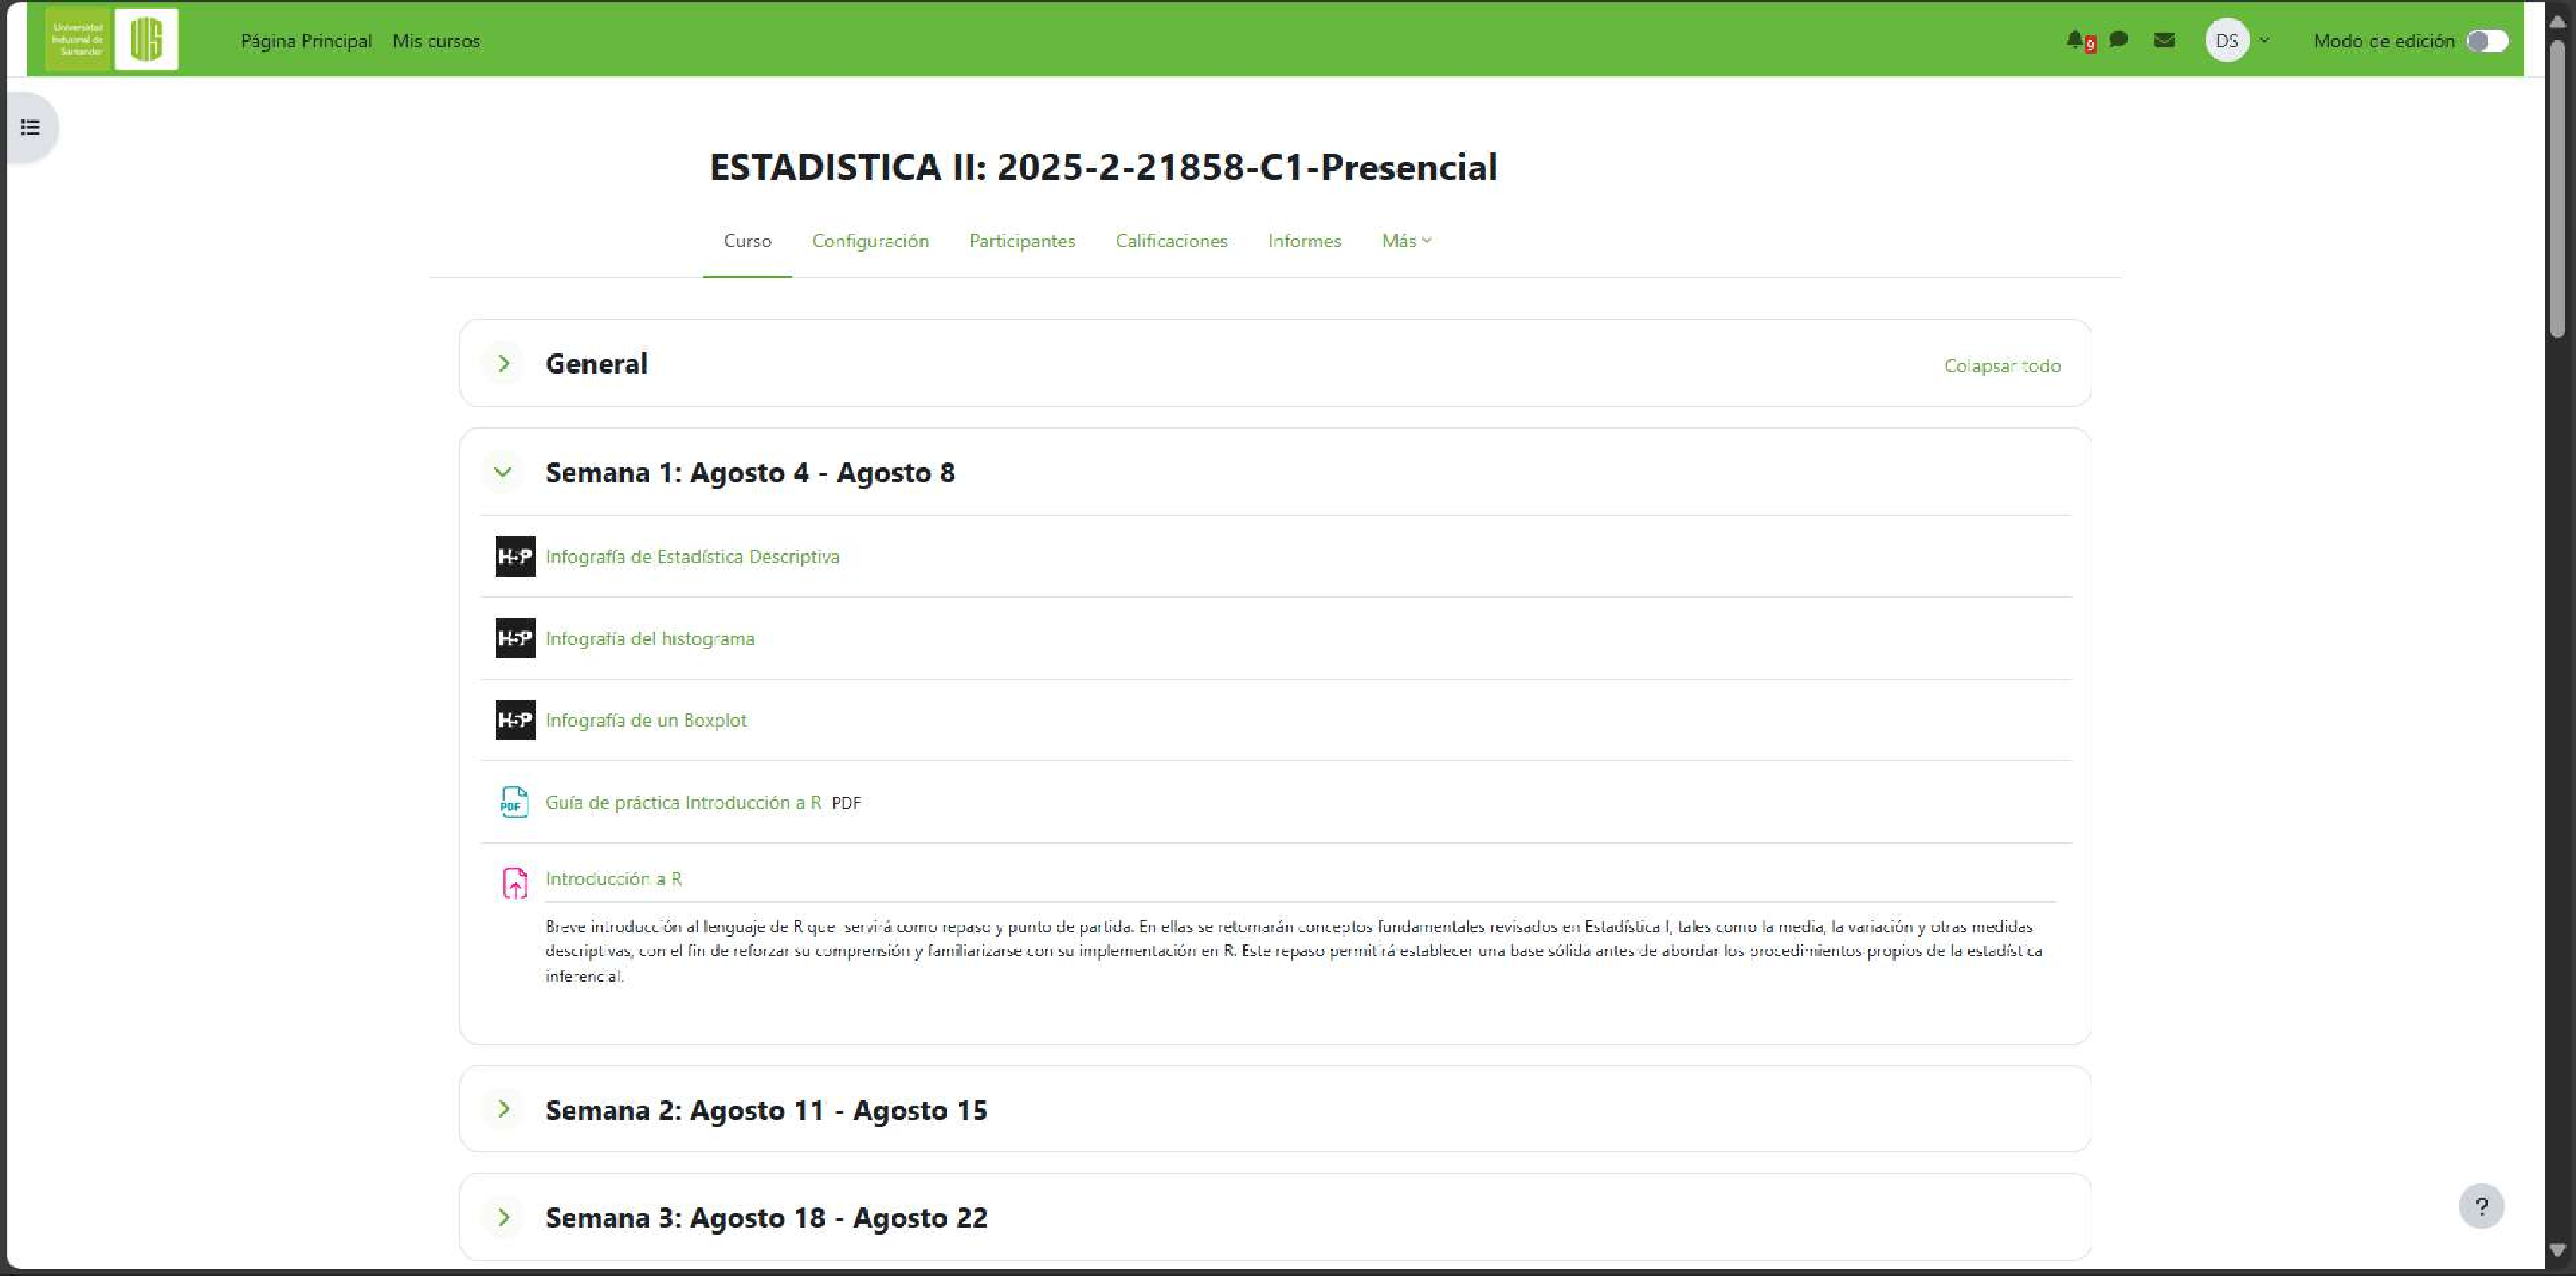
\includegraphics[width=0.8\textwidth]{Figs/Moodle.pdf}
	\label{fig:Moodle}
	\\Fuente: Captura de pantalla del curso en Moodle.
\end{figure}

\newpage

Vinculado a través de la plataforma, se utilizó el entorno virtual para realizar de ejercicios prácticos en R y Python, lo que permitió a los estudiantes aplicar de manera directa los conceptos teóricos aprendidos. Esta integración favoreció la resolución de los problemas estadísticos mediante programación, promoviendo el desarrollo de habilidades analíticas y computacionales, así como el aprendizaje activo y la comprensión profunda de los métodos estadísticos.

Un ejemplo de ello fue la implementación del método \textit{bootstrap} para la estimación de la mediana y el uso del \textit{skewness} como criterio para decidir si emplear el estimador normal o el de percentiles. A través de esta actividad, los estudiantes pudieron seguir paso a paso el proceso de remuestreo, calcular el sesgo (\textit{Bias}), el error estándar (\textit{SE}) y finalmente construir intervalos de confianza al 95 \%. El código utilizado fue el siguiente:

\renewcommand{\lstlistingname}{Código}
\begin{lstlisting}[language=R, caption={Implementación del método Bootstrap en R}]
# Semilla de reproducibilidad
set.seed(21)
x <- c(0.5, 1, 0.75, 1.2, 0.9, 1.1, 2, 3, 4, 5, 6, 8, 10, 
       0.6, 0.7, 0.8, 0.9, 1.0, 1.3, 1.5)
B <- 1500
orig <- median(x)
n <- length(x)

boots <- numeric(B)
for(i in 1:B){
  s <- sample(x, size = n, replace = TRUE)
  boots[i] <- median(s)
}
bias <- round(mean(boots) - orig, 4)
se_boot <- round(sd(boots), 4)
skew_boot_n <- ((boots-mean(boots))/(se_boot))^3
skew_boot <- round(mean(skew_boot_n), 4)

alpha <- 0.05
method <- ifelse(abs(skew_boot) < 0.5, "normal", "percentil")
if(method == "normal"){
  z <- qnorm(1-alpha/2)
  ci_lower <- orig - z * se_boot
  ci_upper <- orig + z * se_boot
} else {
  ci <- quantile(boots, c(alpha/2, 1 - alpha/2))
  ci_lower <- ci[1]; ci_upper <- ci[2]
}

cat("Original mediana:", orig, "\n")
cat("Bias:", bias, "\n")
cat("SE:", se_boot, "\n")
cat("Skewness:", skew_boot, "\n")
cat("Metodo elegido:", method, "\n")
cat("IC:", "[",ci_lower, ";", ci_upper,"]", "\n")
\end{lstlisting}

La actividad ayudó a reforzar el concepto de intervalo de confianza y la estimación mediante remuestreo, además de permitir a los estudiantes experimentar cómo estas técnicas estadísticas se aplican realmente a través de la programación. De esta manera, los resultados no quedaron en un simple cálculo, sino que fueron comprendidos e interpretados dentro de un contexto académico práctico y aplicado.

Los graders automáticos se integraron al aula virtual con el propósito de ofrecer a los estudiantes una retroalimentación inmediata de las prácticas. Gracias a esta herramienta, los estudiantes pudieron comprobar en tiempo real la validez de sus respuestas como se observa en la Figura \ref{fig:Colab}, identificar errores y comprender de manera más clara los pasos necesarios para llegar a la solución correcta. Así, además de agilizar la evaluación, se promovió una participación más autónoma y activa; los estudiantes tenían la oportunidad de corregir desde su propia experiencia.

\begin{figure}[ht]
	\centering
	\captionof{figure}{ \\ \vspace{0.5cm} Desarrollo tecnológico del ambiente virtual. \textbf{Calificador de las prácticas}.}
	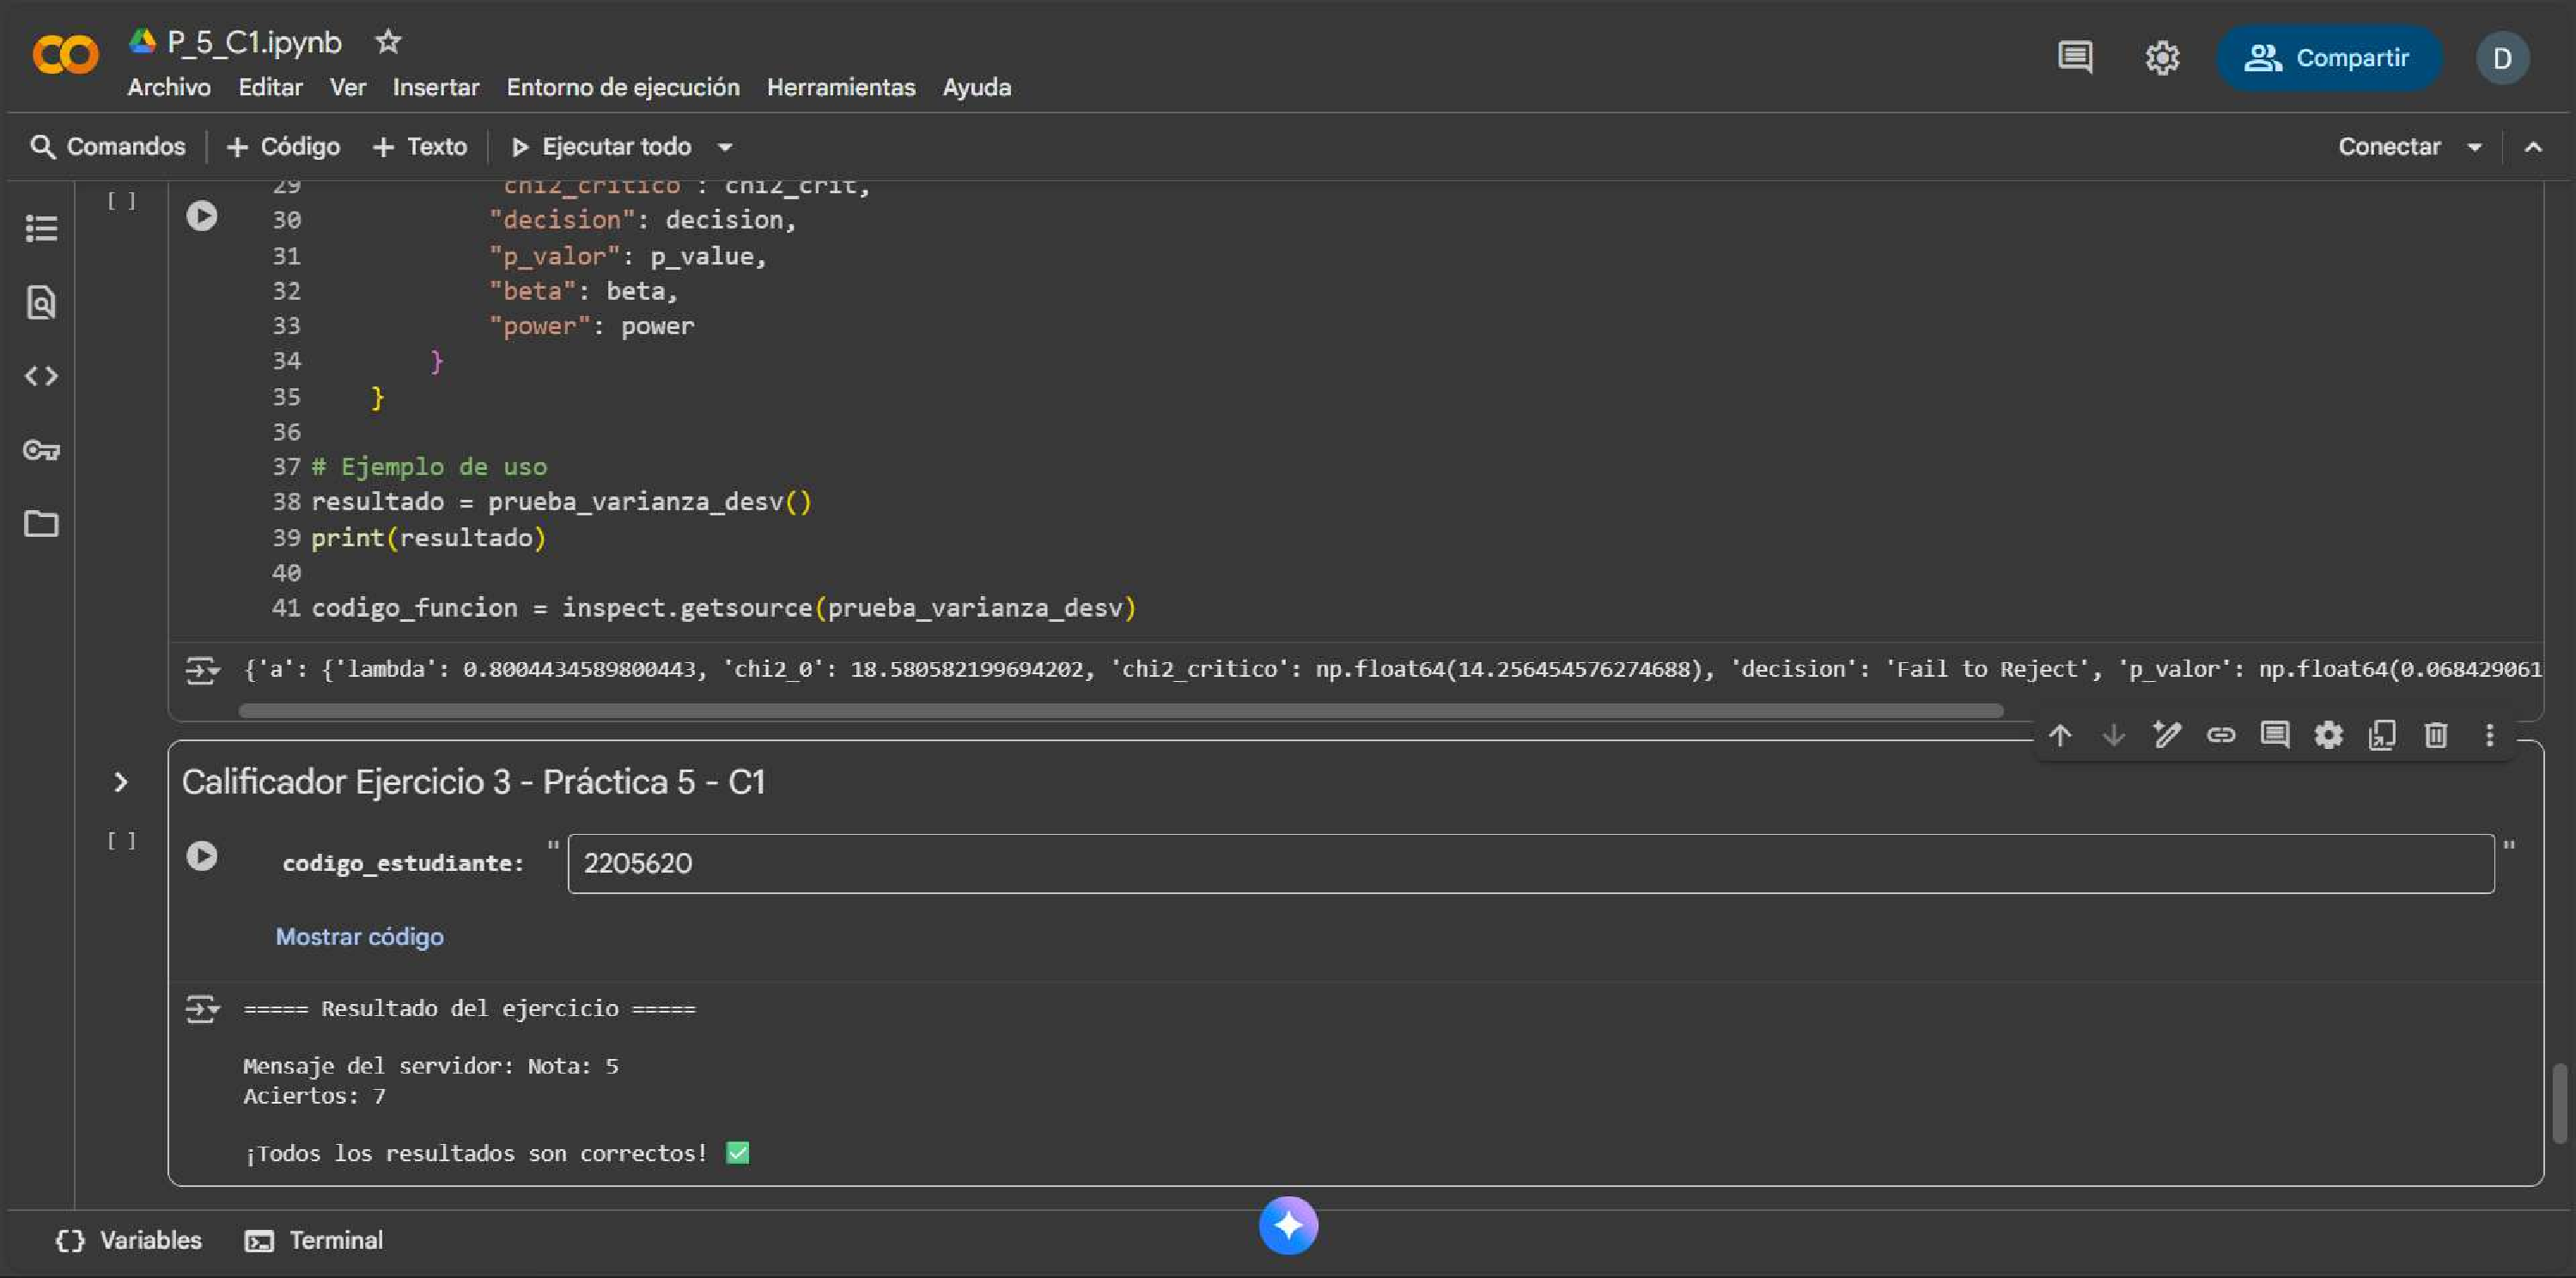
\includegraphics[width=1\textwidth]{Figs/Colab.pdf}
	\label{fig:Colab}
	\\Fuente: Captura de pantalla del mensaje del calificador en el Notebook.
\end{figure}
\newpage
Se implementó el plugin \textit{Safe Exam Browser (SEB)} en los cuestionarios del curso. Esta herramienta permite bloquear el acceso a otras aplicaciones, navegadores o páginas web mientras los estudiantes realizan los ejercicios, asegurando que cada cuestionario se responda de manera individual y bajo condiciones controladas como se muestra en la Figura \ref{fig:SEB} (el cual no permite realizar captura de pantalla). Aportando ventajas significativas como:

\begin{itemize}
    \item \textbf{Prevenir distracciones y accesos no autorizados:} los estudiantes no podían navegar fuera del entorno de evaluación, lo que permitió mantener su atención centrada en los ejercicios.
    \item \textbf{Fortalecer la confiabilidad de los resultados:} los datos reflejaron únicamente el desempeño individual de cada estudiante, ofreciendo información más precisa sobre su aprendizaje.
\end{itemize}

Gracias a estas características, SEB no solo reforzó la seguridad de los cuestionarios, sino que también contribuyó a crear un entorno más confiable y justo para los estudiantes, promoviendo una experiencia de aprendizaje más seria y comprometida.

\begin{figure}[ht]
	\centering
	\captionof{figure}{ \\ \vspace{0.5cm} Desarrollo tecnológico del ambiente virtual. \textbf{Safe Exam Browser}.}
	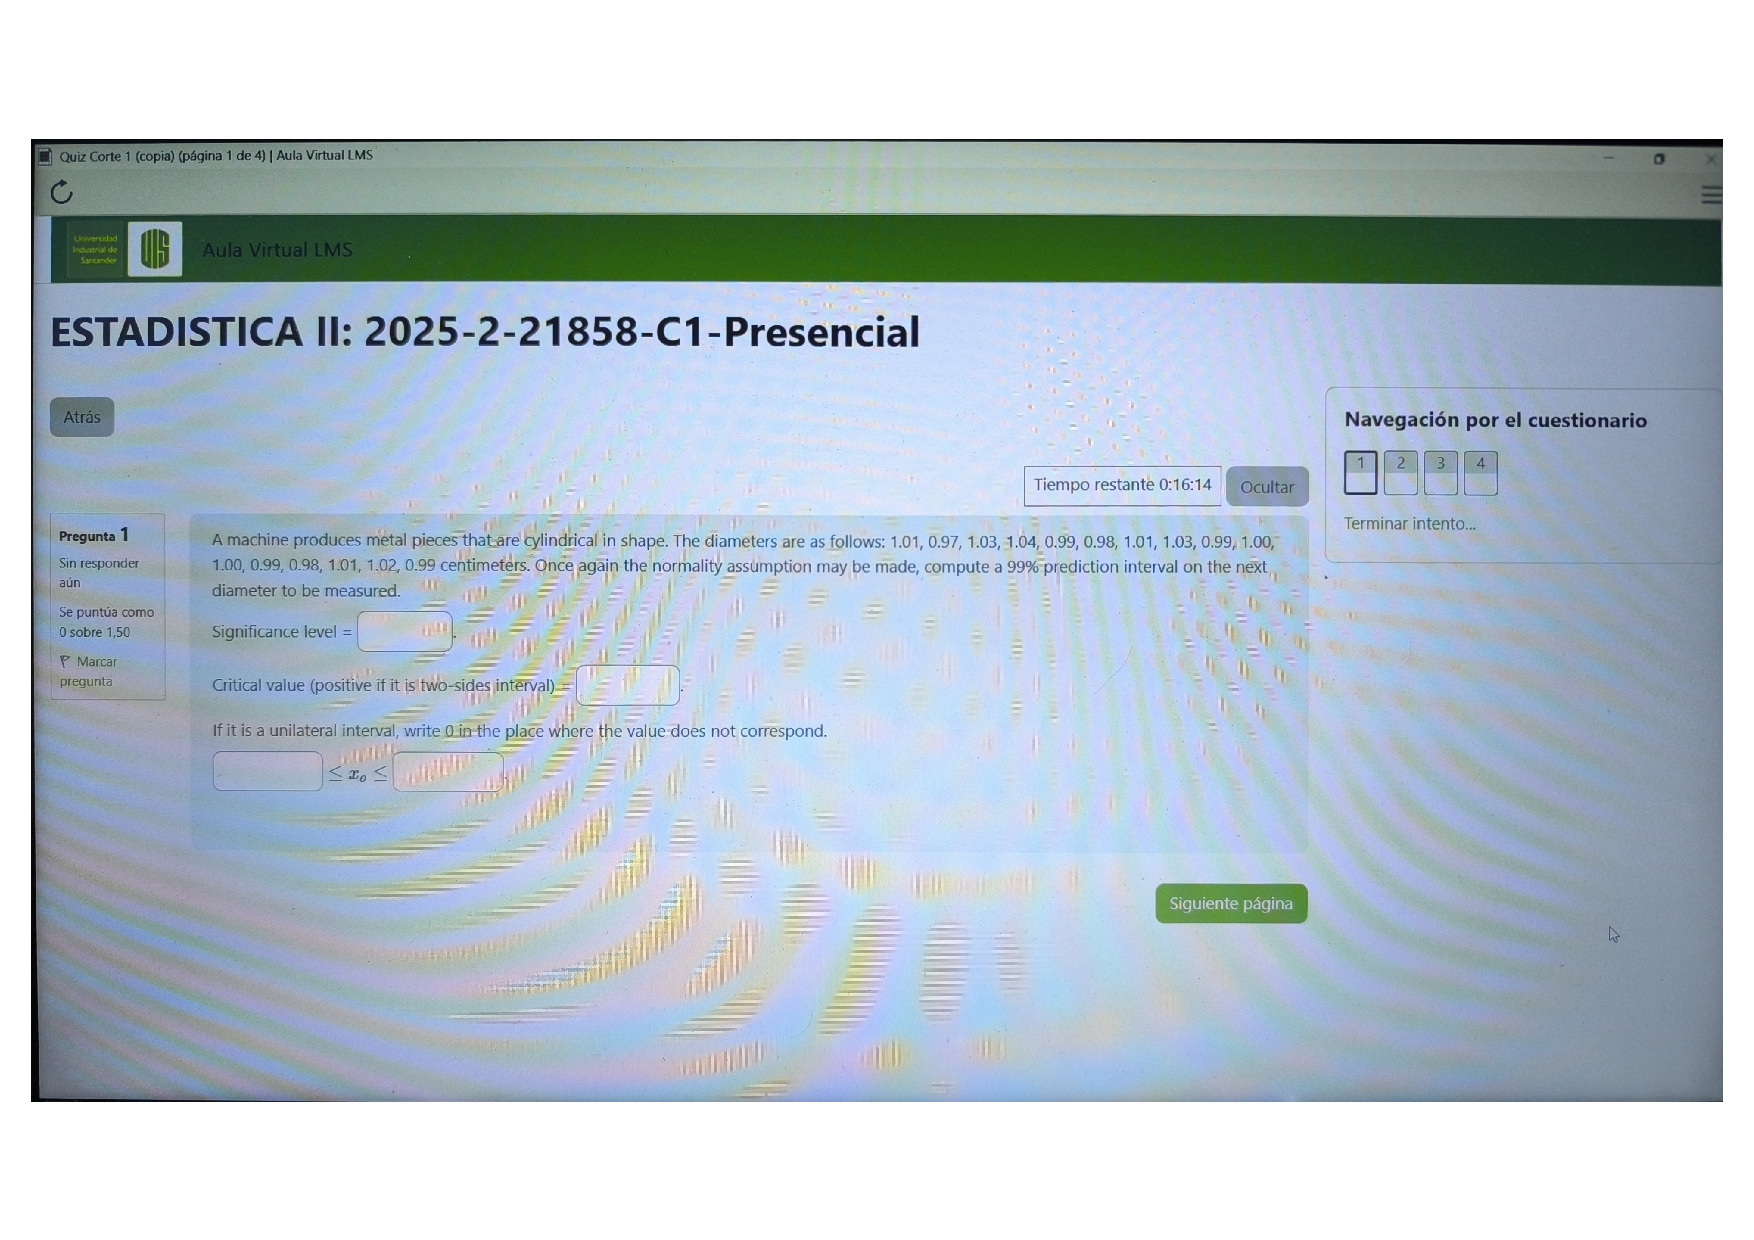
\includegraphics[width=0.8\textwidth]{Figs/SEB.pdf}
	\label{fig:SEB}
	\\Fuente: Foto de un cuestionario en Safe Exam Browser.
\end{figure}

\section{Infraestructura tecnológica implementada}

La infraestructura tecnológica diseñada para soportar el ambiente virtual de aprendizaje se estructuró bajo un modelo basado en contenedores \textit{Docker}, lo que permitió separar los distintos servicios y garantizar su portabilidad y escalabilidad (Anexo \ref{anexo:repositorio}). El despliegue general se gestionó mediante el archivo \texttt{docker-compose.yml} en un computador personal de 12 GB de ram en un sistema operativo UBUNTU de Linux, que coordinó la ejecución simultánea de cada servicio como se muestra en la Figura \ref{fig:AVA}. La organización de los servicios se estructuró de la siguiente manera:

\begin{figure}[ht]
	\centering
	\captionof{figure}{ \\ \vspace{0.5cm} Infraestructura tecnológica implementada. \textbf{Arquitectura tecnológica del Ambiente Virtual de aprendizaje}.}
	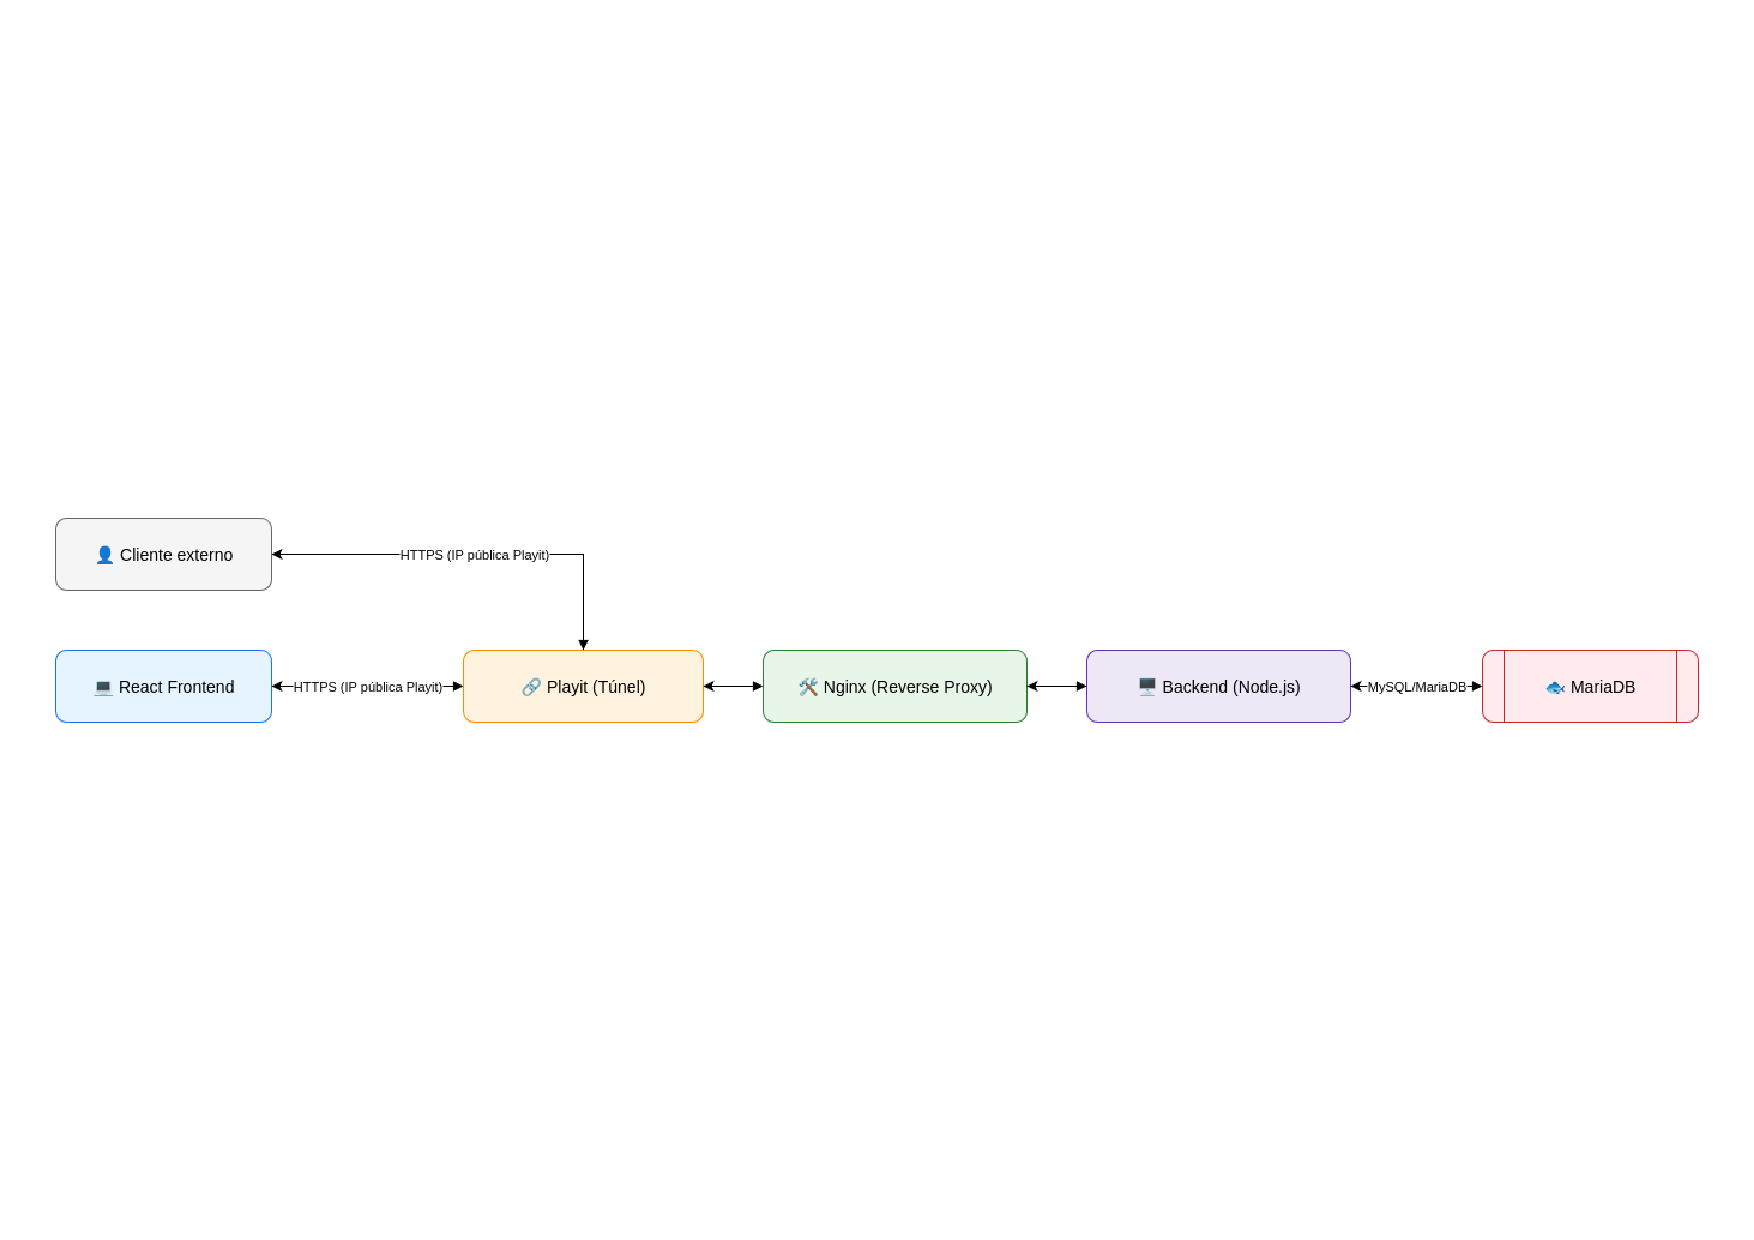
\includegraphics[width=1\textwidth]{Figs/Arquitectura_AVA.pdf}
	\label{fig:AVA}
	\\Fuente: Elaboración propia según el árbol de estructura de servicios.
\end{figure}

\subsection{Backend}
\begin{itemize}
    \item Contiene la lógica principal del sistema desarrollada en \textit{Node.js}.
    \item El archivo \texttt{server.js} y la carpeta \texttt{src/app.js} gestionan la configuración base del servidor.
    \item En la carpeta \texttt{controllers} se desarrollaron los controladores para las diferentes prácticas (\texttt{prac1.controller.js}, \texttt{prac2.controller.js}, etc.), el manejo de estudiantes y la comunicación con la interfaz de frontend.
    \item En \texttt{routes} se definieron las rutas para estudiantes, cuestionarios y la interacción con el frontend.
    \item La carpeta \texttt{config/db.js} centralizó la conexión con la base de datos.
\end{itemize}

\subsection{Frontend}
\begin{itemize}
    \item Implementado con \textit{React}, contenía la interfaz con la que interactuaron los practicantes y el docente.
    \item En la carpeta \texttt{components} se construyeron elementos como \texttt{Grupos.js}, \texttt{Semanas.js} y \texttt{DetalleEstudiante.js}, que organizaron la presentación de la información académica como se puede observar en la Figura \ref{fig:Detalles}.
    
	\begin{figure}[ht]
		\centering
		\captionof{figure}{ \\ \vspace{0.5cm} Infraestructura tecnológica implementada. \textbf{Detalle del envío en frontend}.}
		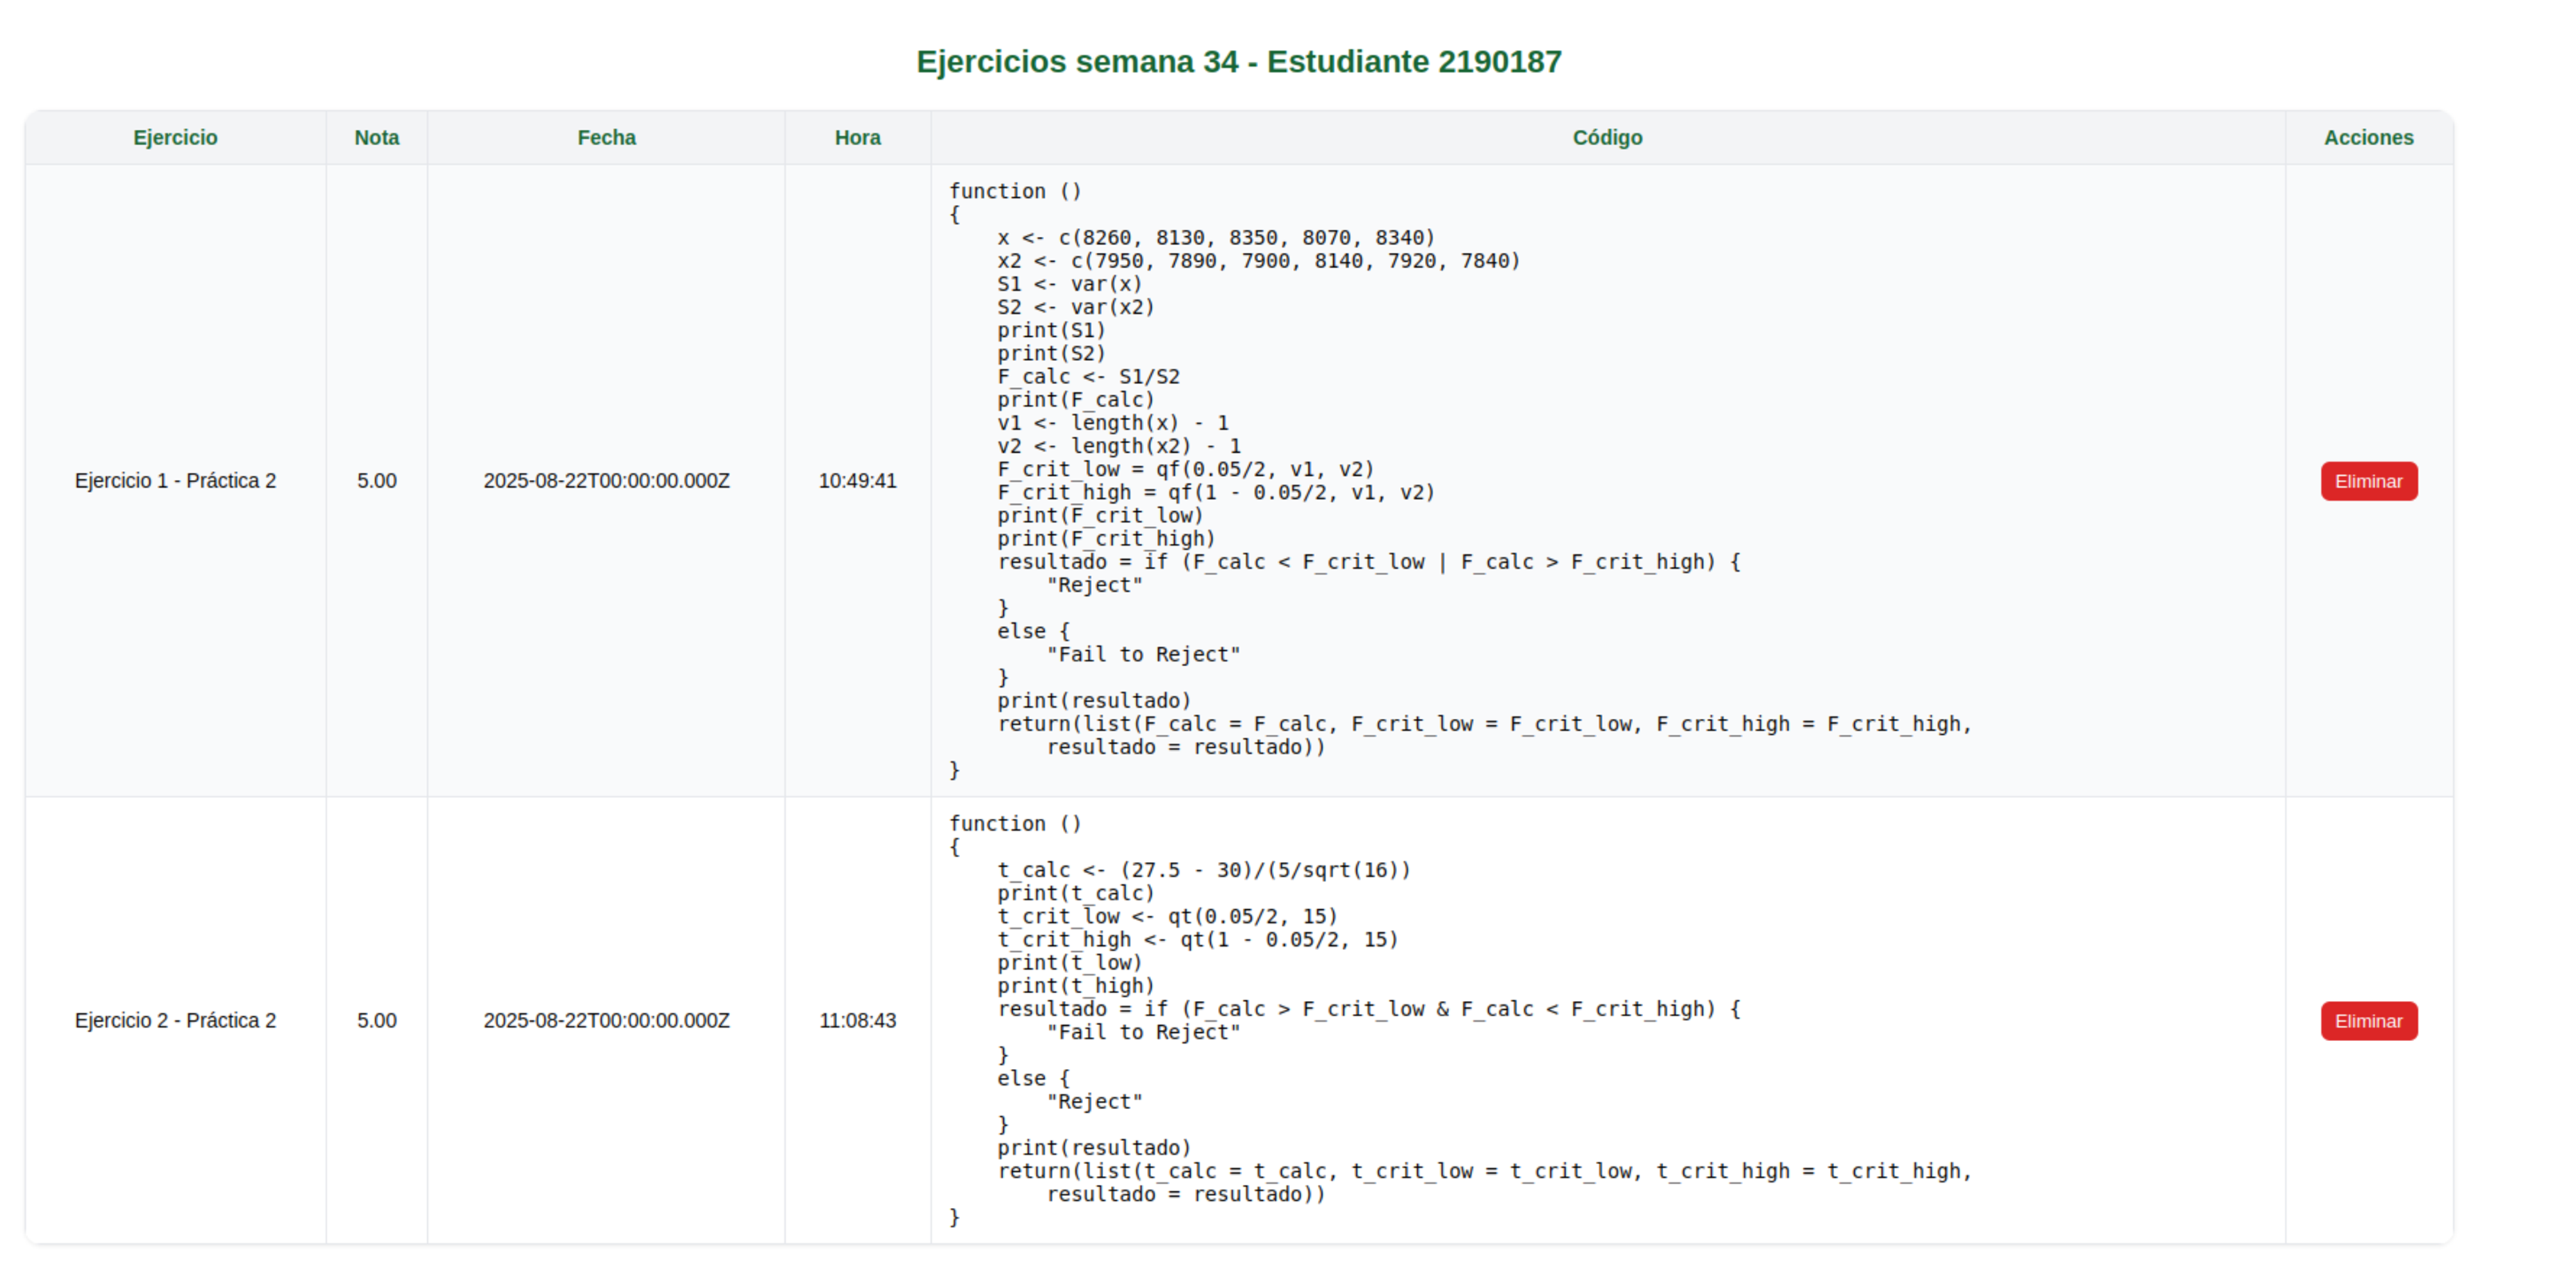
\includegraphics[width=0.9\textwidth]{Figs/Detalles_practica.pdf}
		\label{fig:Detalles}
		\\Fuente: Captura de pantalla de los detalles del código realizada por los estudiantes.
	\end{figure}

	\item Los estilos \texttt{CSS} asociados (\texttt{Grupos.css}, \texttt{Semanas.css}, \texttt{DetalleEstudiantes.css}) se diseñaron para lograr una visualización limpia y funcional como muestra la Figura \ref{fig:Interfaz}.
    
	\begin{figure}[ht]
		\centering
		\captionof{figure}{ \\ \vspace{0.5cm} Infraestructura tecnológica implementada. \textbf{Interfaz de notas}.}
		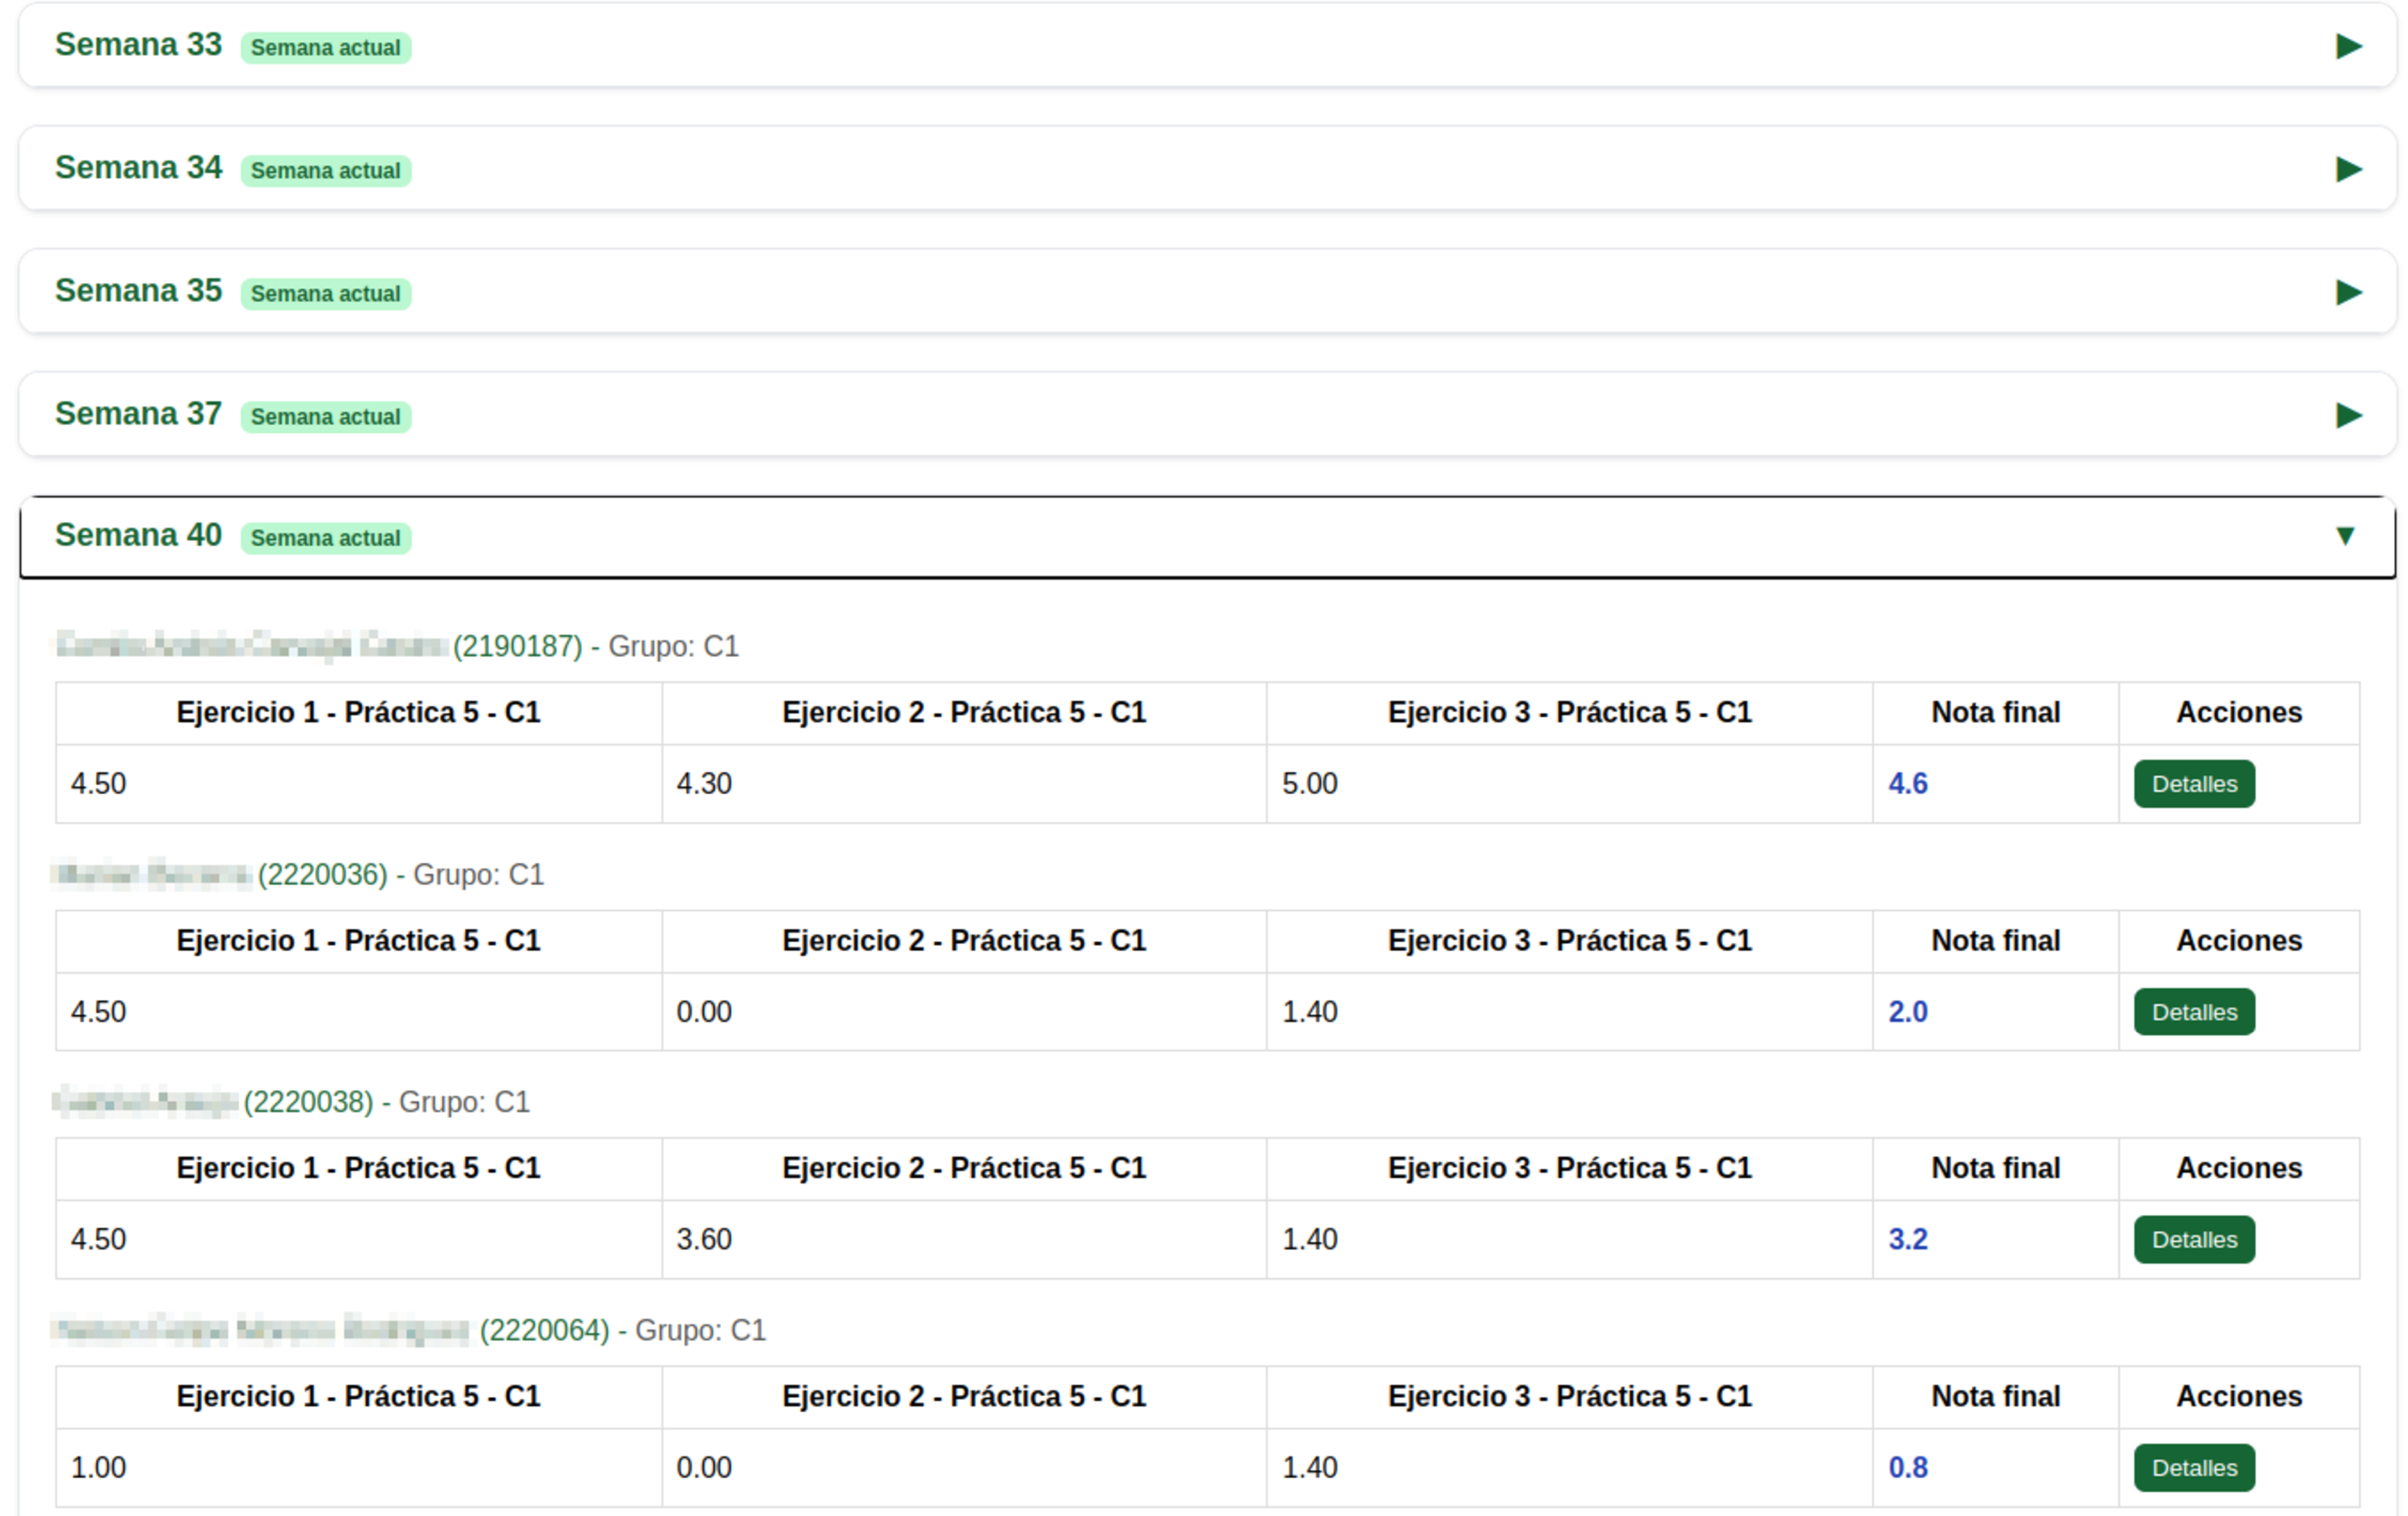
\includegraphics[width=0.83\textwidth]{Figs/Interfaz _de_notas.pdf}
		\label{fig:Interfaz}
		\\Fuente: Captura de pantalla de la visualización de las notas.
	\end{figure}
	
	\item El despliegue del \textit{frontend} se gestionó mediante un \texttt{Dockerfile}, asegurando que la interfaz se integrara de manera coherente al ecosistema.
\end{itemize}

\subsection{Base de Datos}
\begin{itemize}
    \item Se utilizó \textit{MariaDB} como sistema gestor, con inicialización automática mediante el archivo \texttt{init.sql}.
    \item La persistencia se garantizó con el volumen \texttt{mariadb\_data}.
\end{itemize}

\subsection{Nginx}
\begin{itemize}
    \item Funcionó como servidor web y proxy inverso, controlando el acceso externo al sistema.
    \item El archivo \texttt{nginx.conf} definió las reglas de enrutamiento.
    \item La carpeta \texttt{certs} almacenó los certificados de seguridad (\texttt{fullchain.pem} y \texttt{privkey.pem}), junto con la configuración del certificado SAN (\texttt{san.cnf}) para habilitar la navegación segura mediante \texttt{HTTPS}.
    \item Los registros de acceso y errores (\texttt{logs/access.log}, \texttt{logs/error.log}) facilitaron la monitorización del sistema.
	\item Es importante destacar que la configuración de \textbf{Nginx} incluyó la directiva:
    
    \begin{itemize}
        \item \texttt{limit\_req\_zone \$binary\_remote\_addr zone=api\_limit:10m rate=10r/s;}
    \end{itemize}
    
    Esta directiva limita la cantidad de solicitudes permitidas por cada dirección IP a un máximo de 10 por segundo. Con ello, se establece un mecanismo de control de tráfico que evita la sobrecarga del servidor y contribuye a la mitigación de ataques de \textbf{denegación de servicio distribuida (DDoS)}, fortaleciendo la seguridad y estabilidad de la aplicación.
\end{itemize}

\subsection{Playit.gg}
\begin{itemize}
    \item Durante la implementación de los grupos piloto, se utilizó este servicio para establecer túneles seguros y exponer temporalmente los servicios como en la Figura \ref{fig:Playit}.
    
	\begin{figure}[ht]
		\centering
		\captionof{figure}{ \\ \vspace{0.5cm} Infraestructura tecnológica implementada. \textbf{Dashboard de los túneles utilizados en Playit.gg}.}
		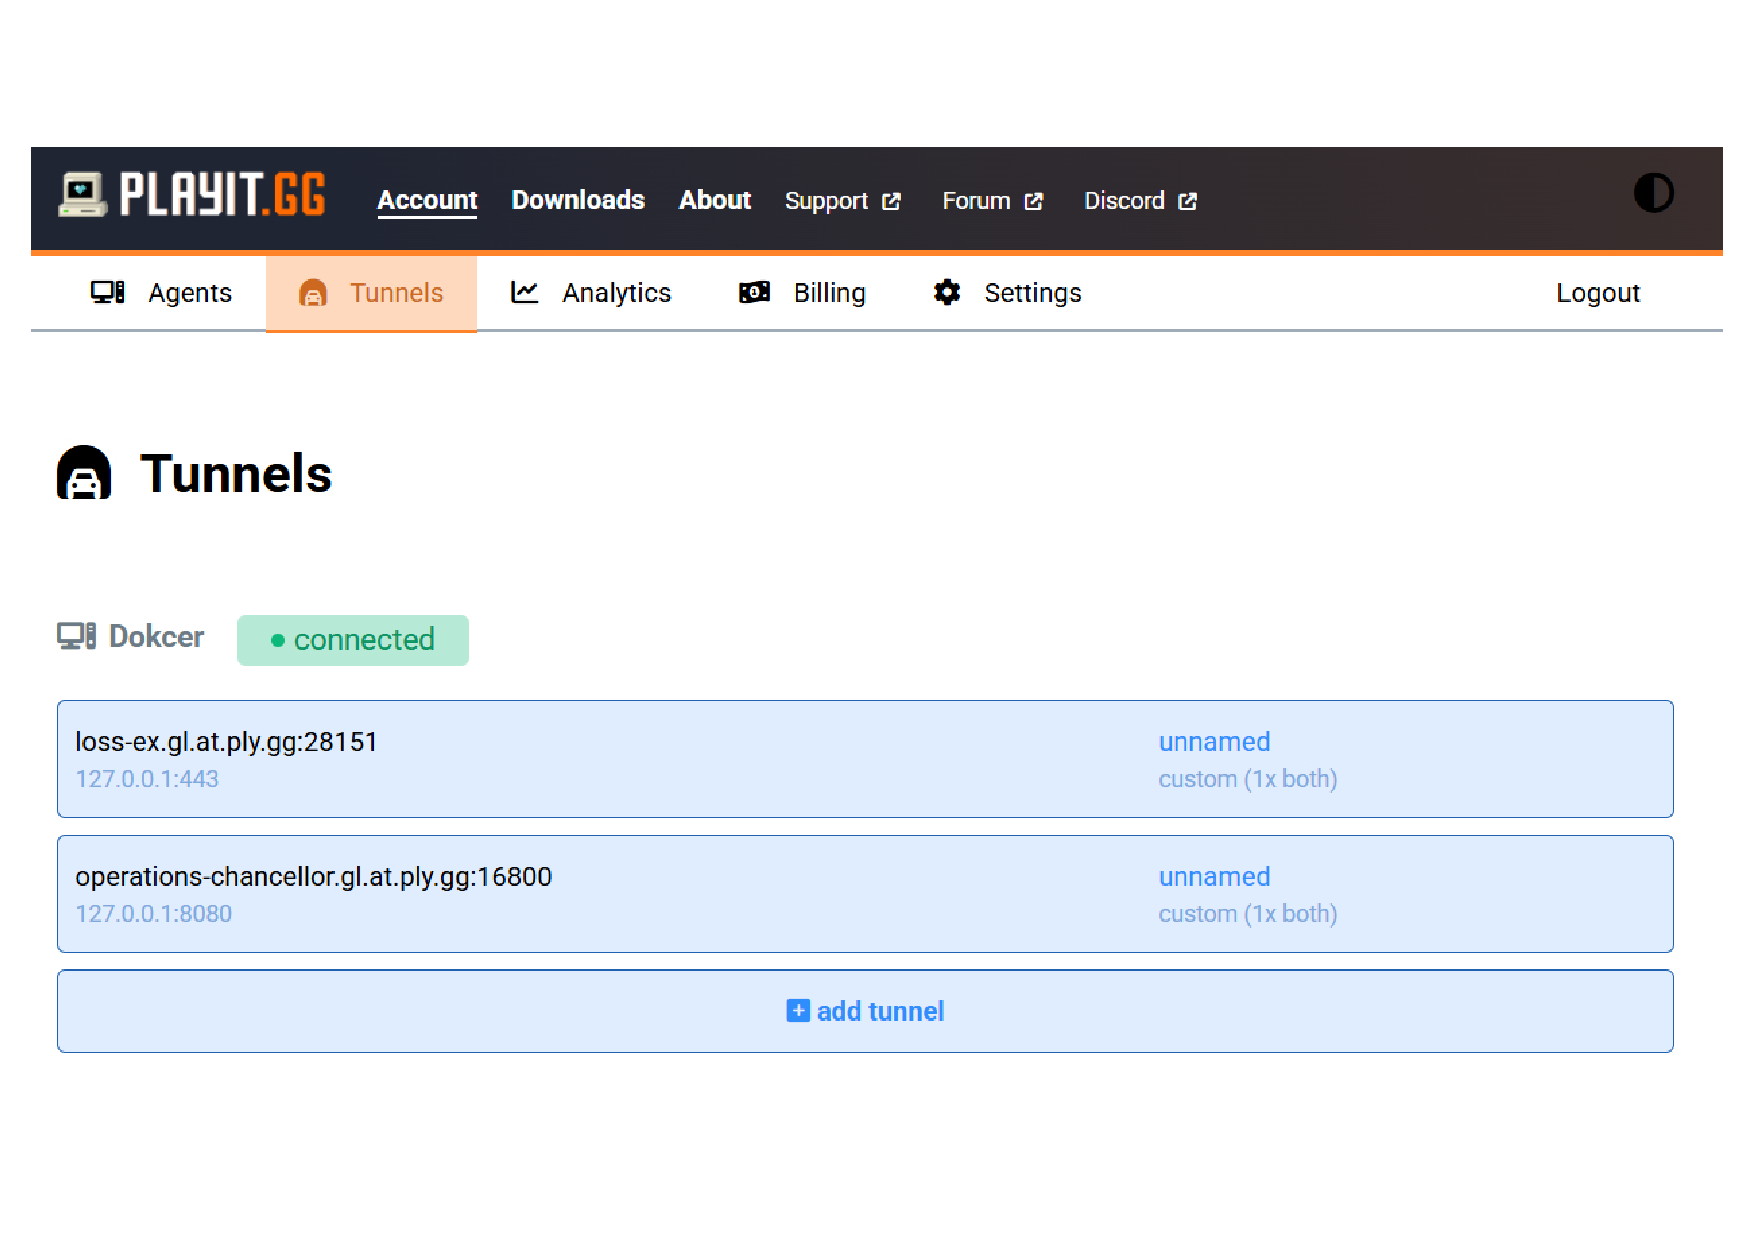
\includegraphics[width=0.83\textwidth]{Figs/dashboard playit.gg.pdf}
		\label{fig:Playit}
		\\Fuente: Captura de pantalla del dashboard de los túneles de Playit.
	\end{figure}
	
	\item Esto garantizó la accesibilidad sin necesidad de un despliegue en un servidor hosting.
\end{itemize}

\subsection{Desempeño de despliegue}

El análisis del desempeño del servidor desplegado mediante el túnel \textit{Playit.gg} mostró que bajo protocolo \textbf{HTTP}, el tiempo de respuesta promedio fue de aproximadamente \textit{0.5 segundos}. Al habilitar \textbf{HTTPS} con certificado autofirmado en \textbf{Nginx}, este tiempo se incrementó a cerca de \textit{1.3 segundos}, debido principalmente a la sobrecarga introducida por el \textbf{handshake TLS}.

Estos resultados evidencian que, aunque el \textbf{backend} y \textbf{Nginx} procesan las solicitudes de manera eficiente, la capa de seguridad genera una latencia adicional. Para mitigar este impacto, se sugiere implementar estrategias de optimización como el \textbf{reuso de sesiones TLS}, el aprovechamiento de \textbf{HTTP/2} y el uso de certificados confiables, por ejemplo de \textit{Let’s Encrypt}, lo cual permitiría mantener altos estándares de seguridad sin comprometer significativamente los tiempos de respuesta.

En conjunto, la infraestructura implementada demuestra un equilibrio entre funcionalidad, seguridad y eficiencia, asegurando un entorno estable y confiable para la interacción académica, la gestión de datos y la ejecución de actividades prácticas dentro del ambiente virtual como se observa en la Figura \ref{fig:DF}.

\newpage

\begin{figure}[ht]
	\centering
	\captionof{figure}{ \\ \vspace{0.5cm} Infraestructura tecnológica implementada. \textbf{Diagrama de flujo que describe el proceso de envío y calificación}.}
	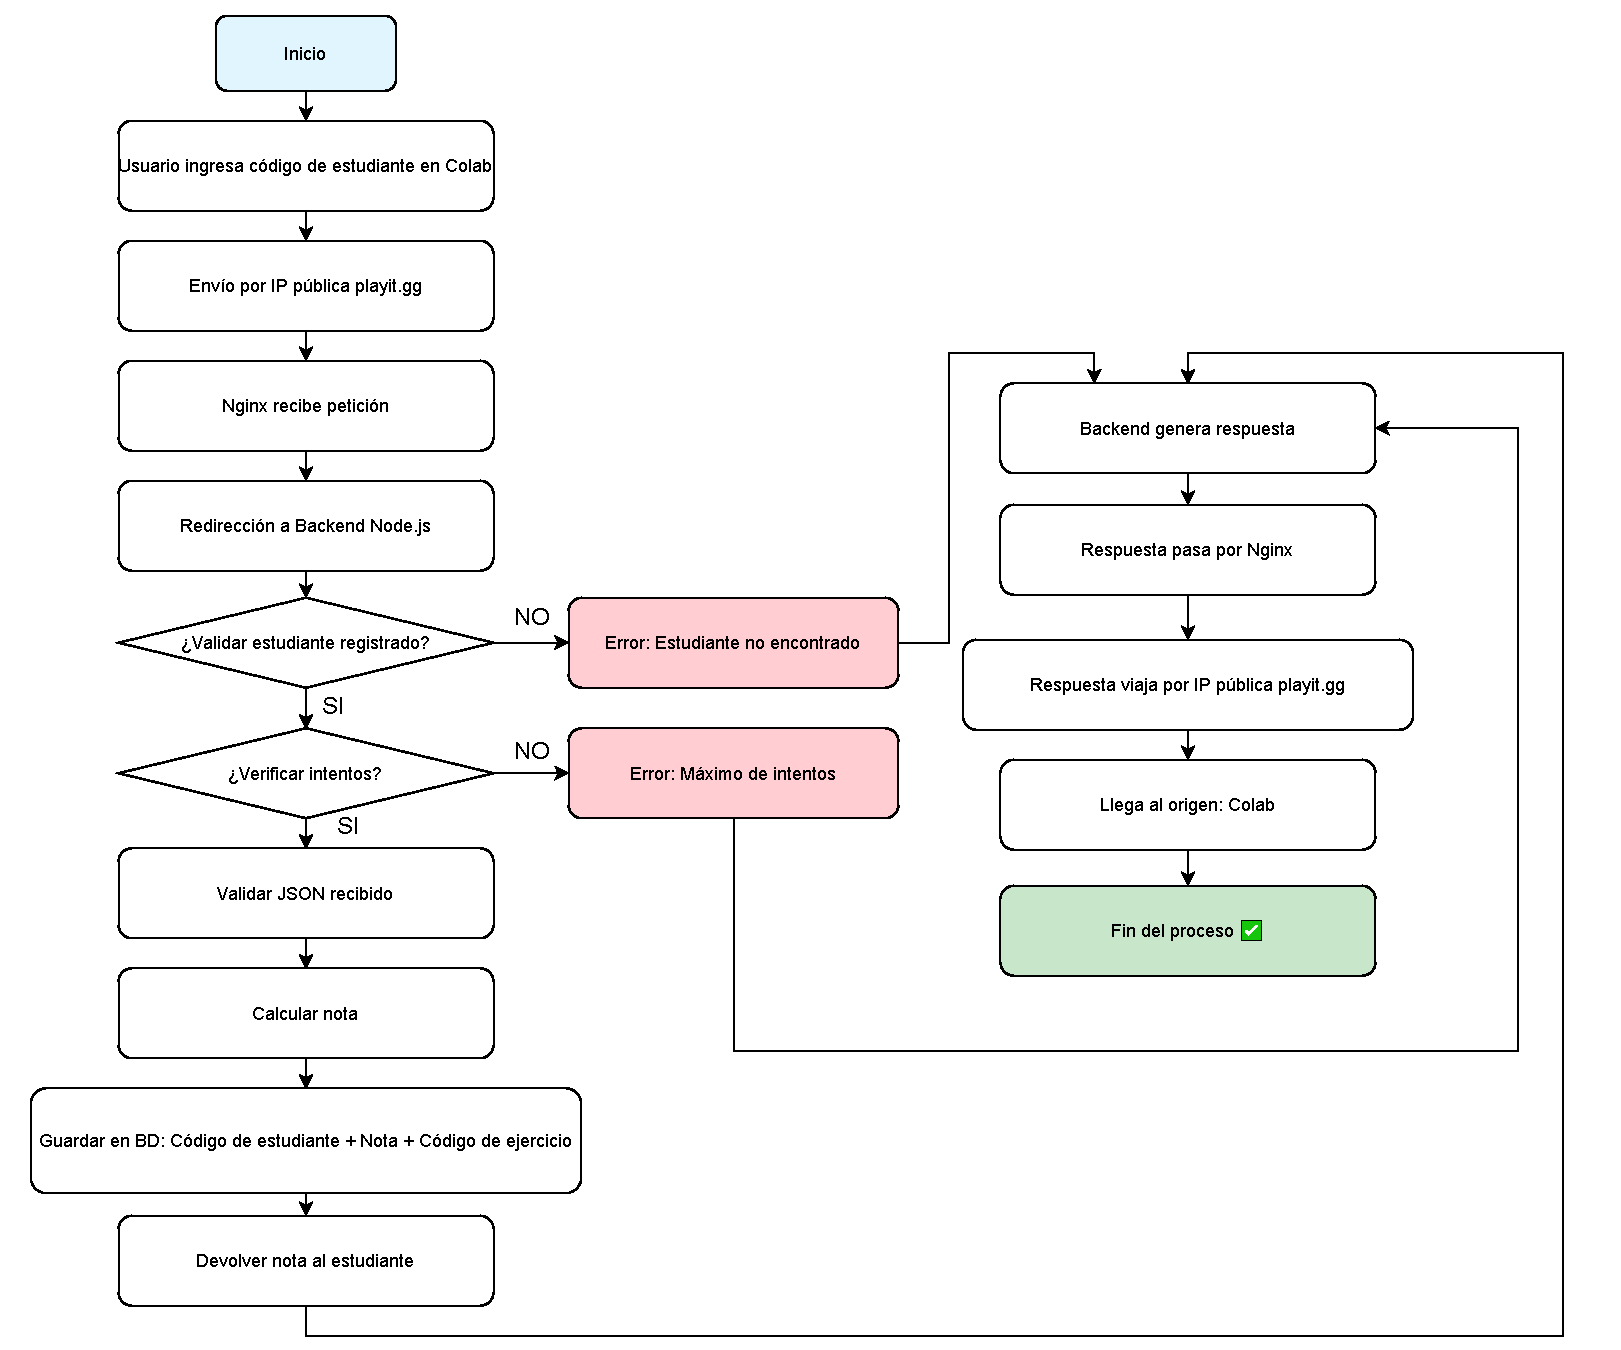
\includegraphics[width=1\textwidth]{Figs/Diagrama_Flujo.pdf}
	\label{fig:DF}
	\\Fuente: Elaboración propia del proceso de envío y calificación.
\end{figure}

\section{Recursos interactivos}

Además de la infraestructura tecnológica y los servicios de programación, el ambiente virtual de aprendizaje integró herramientas digitales especialmente orientadas a enriquecer la experiencia pedagógica de los estudiantes mediante contenidos dinámicos e interactivos (Anexo \ref{anexo:repositorio}).

En este contexto, se hizo uso de \textit{Genially} y \textit{H5P}, plataformas que permitieron diseñar materiales innovadores y atractivos, con el objetivo de facilitar la comprensión de los conceptos teóricos y metodológicos de \textit{Estadística II}. Genially se destinó principalmente a la elaboración de infografías y presentaciones interactivas como se muestran en las Figuras \ref{fig:Pgenially} y \ref{fig:Igenially}, que transformaron información compleja en representaciones visuales claras y accesibles. Estos recursos, una vez integrados en \textit{Moodle}, se convirtieron en un apoyo valioso para los distintos módulos del curso, ya que brindaron a los estudiantes la posibilidad de interactuar con los contenidos y explorar los temas de manera autónoma.

\begin{figure}[ht]
	\centering
	\captionof{figure}{ \\ \vspace{0.5cm} Recursos interactivos. \textbf{Presentación en Genially sobre Intervalos de confianza}.}
	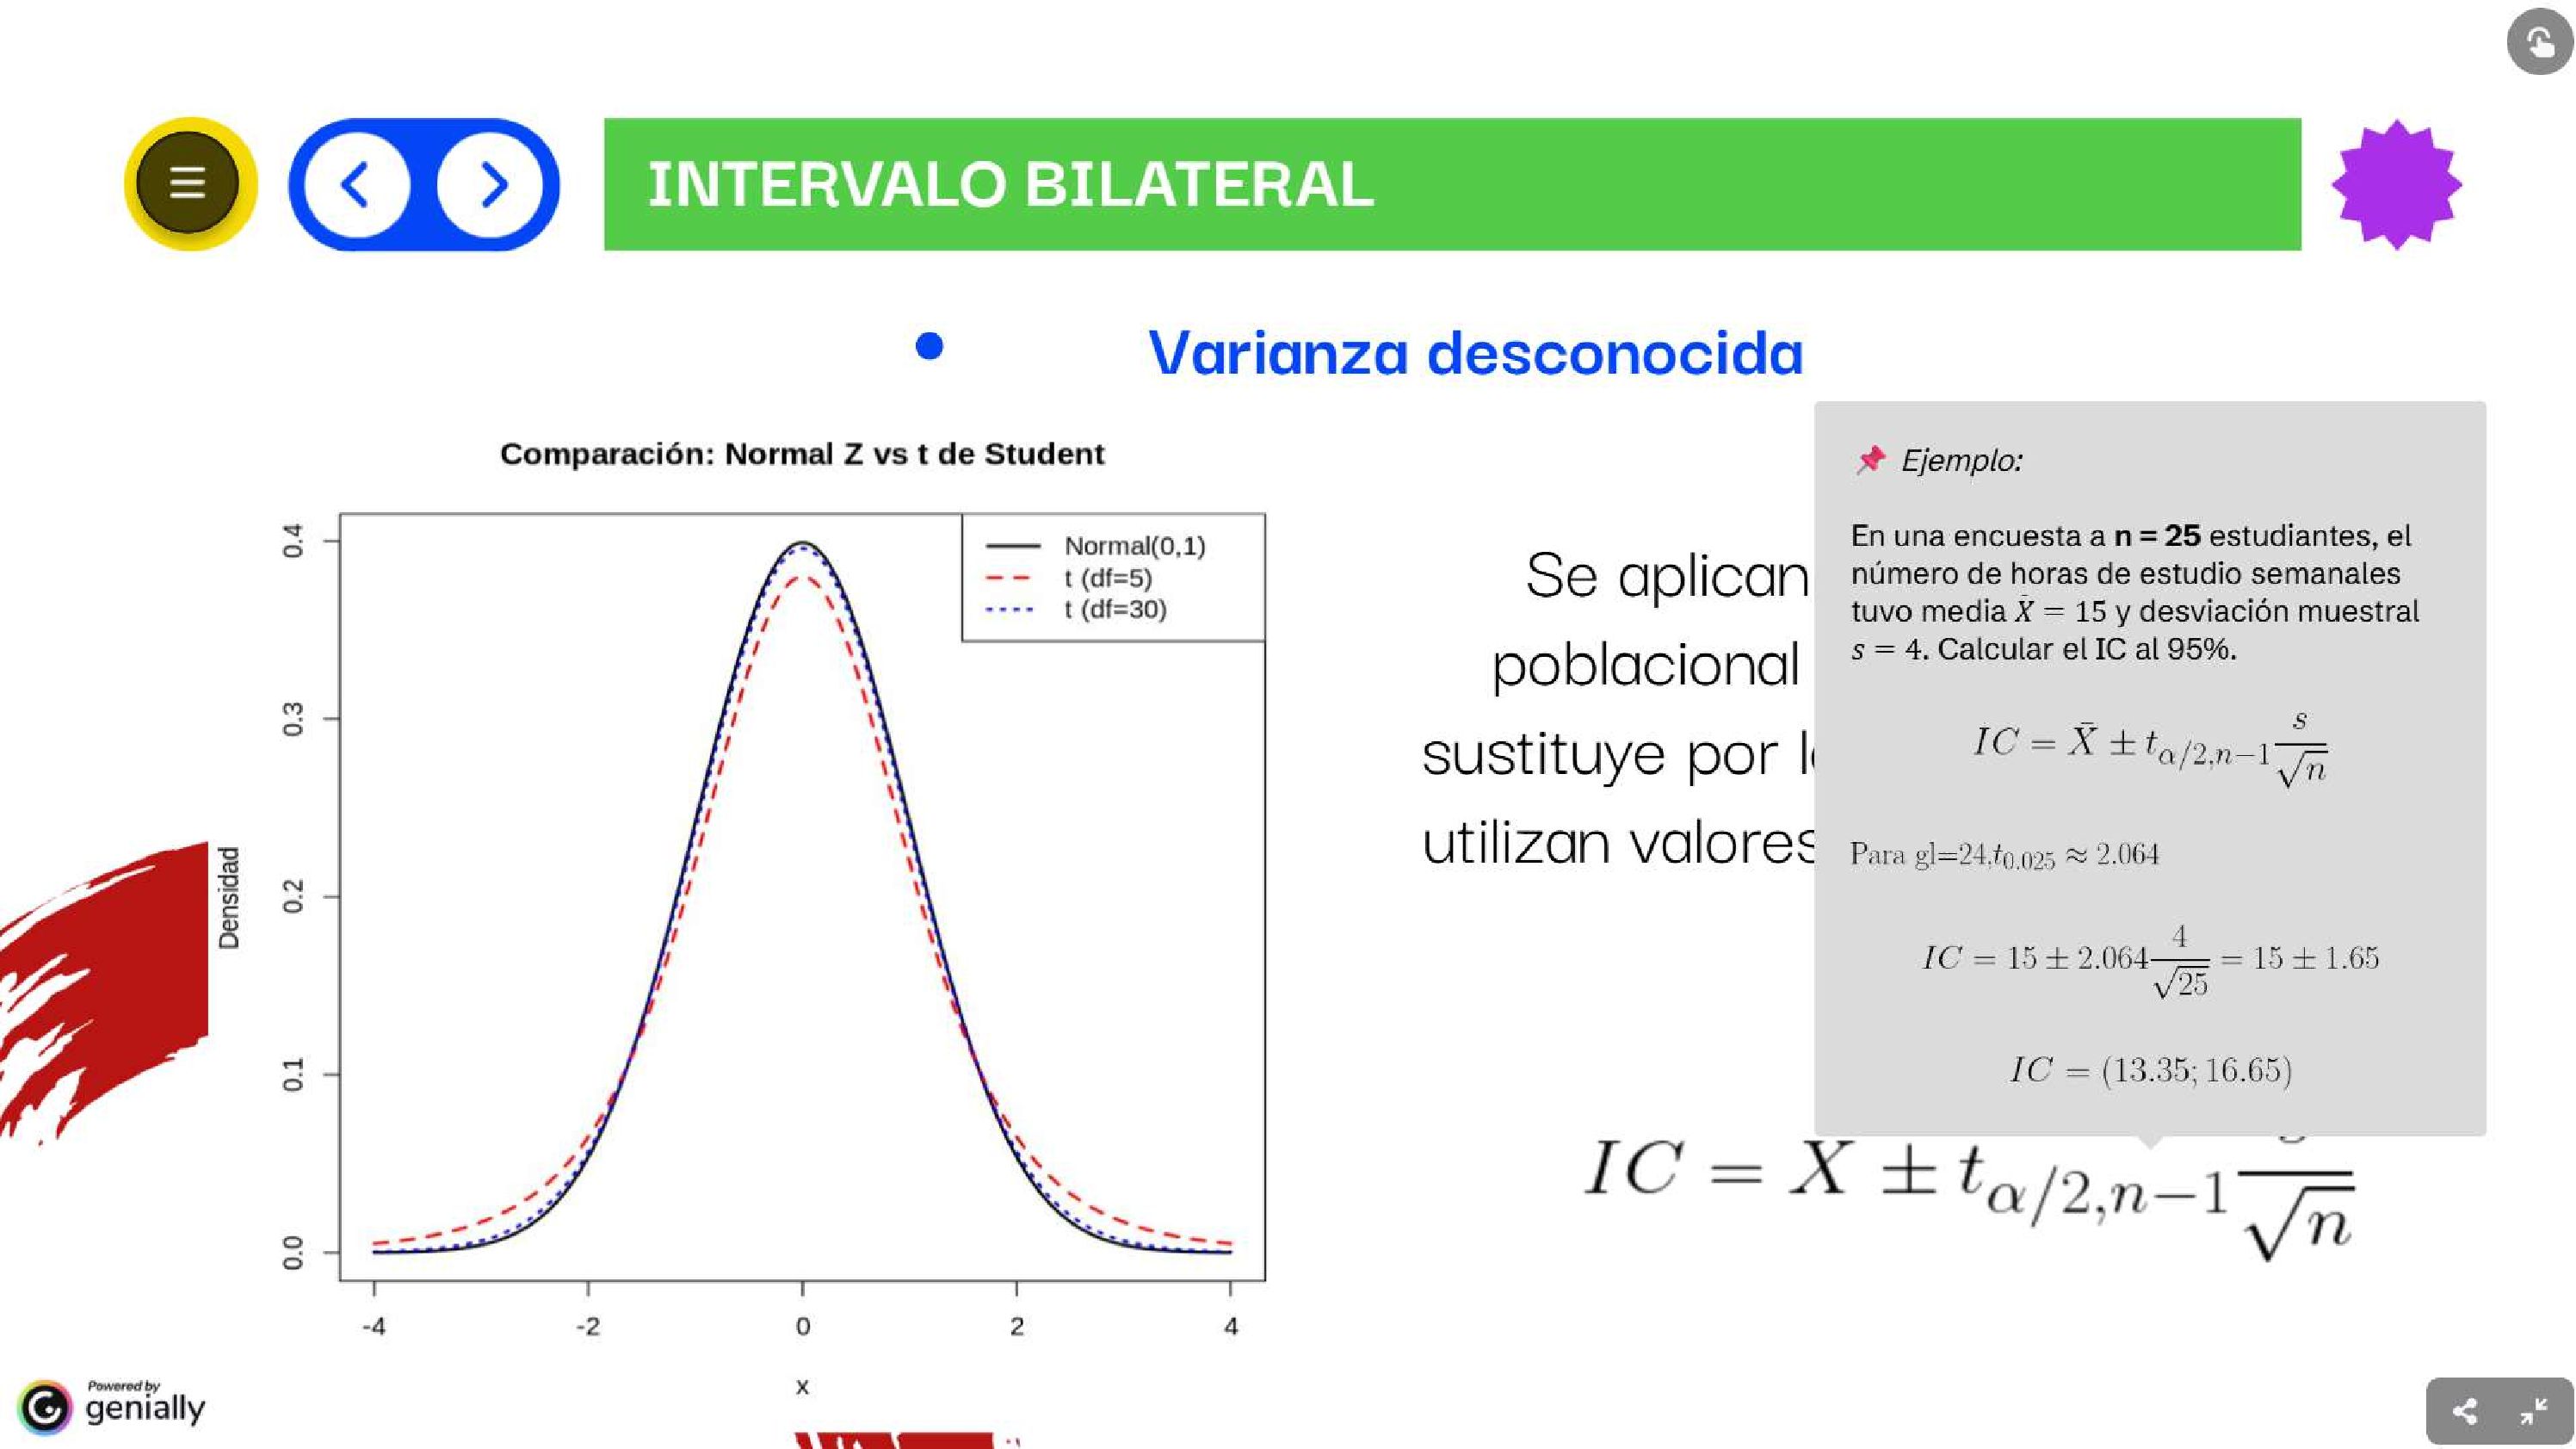
\includegraphics[width=1\textwidth]{Figs/Presentacion_Genially.pdf}
	\label{fig:Pgenially}
	\\Fuente: Captura de pantalla de una presentación en Genially.
\end{figure}

Por su parte, \textit{H5P}, que puede implementarse de forma nativa en \textit{Moodle}, se utilizó para generar infografías y actividades en las primeras clases como se muestra en la Figura \ref{fig:H5P}, contribuyendo a un aprendizaje más activo desde el inicio del curso. En el caso de \textit{Genially}, debido a que no se integra directamente en la plataforma, se recurrió al uso de \textit{iframes} embebidos para incorporar materiales sobre temas complejos, como el Teorema del Límite Central, en los cuales se añadieron diagramas interactivos y simulaciones.

\begin{figure}[ht]
	\centering
	\captionof{figure}{ \\ \vspace{0.5cm} Recursos interactivos. \textbf{Infografía en Genially sobre Bootstrap}.}
	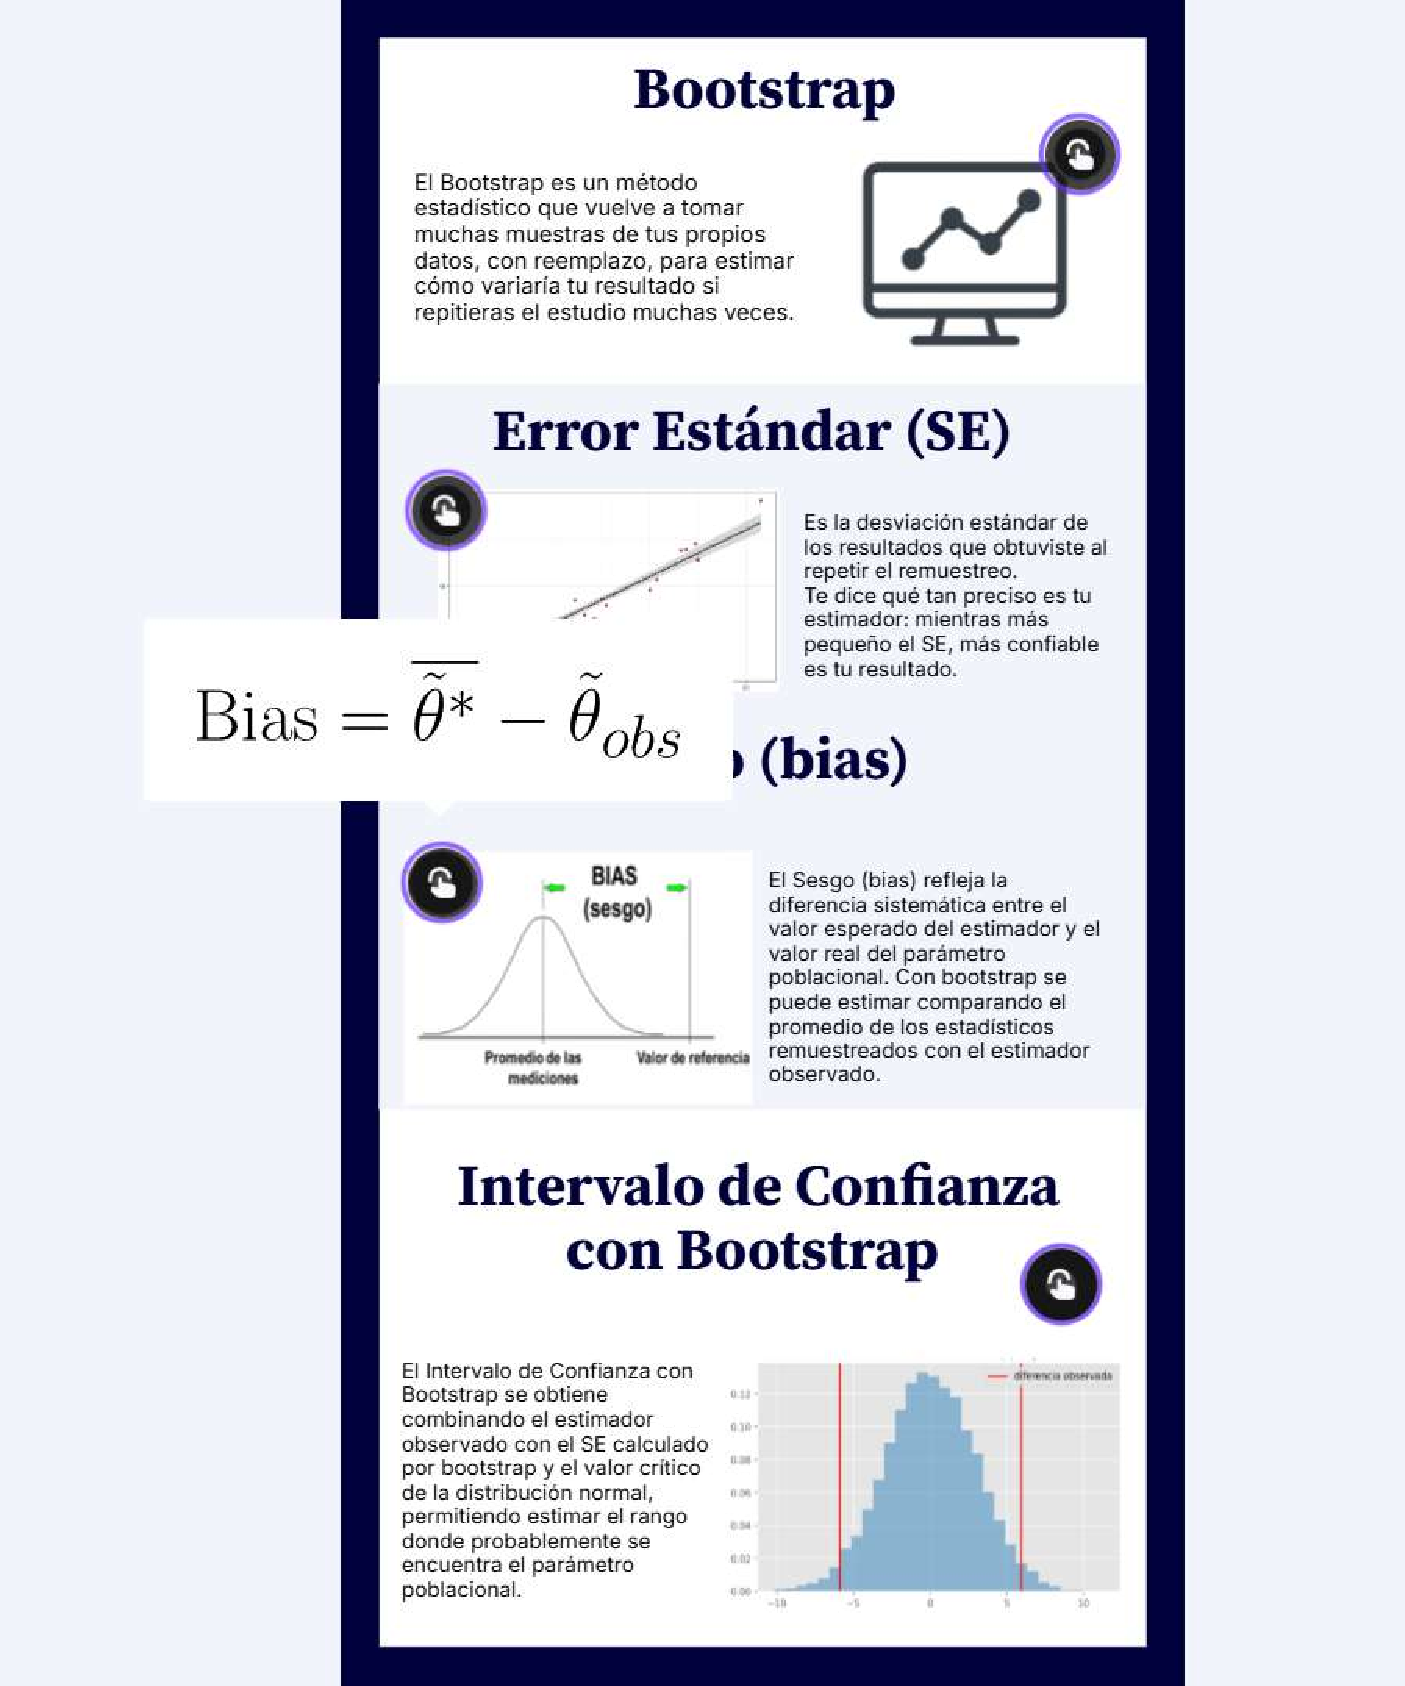
\includegraphics[width=0.65\textwidth]{Figs/Infografia_Genially.pdf}
	\label{fig:Igenially}
	\\Fuente: Captura de pantalla de una infografía en Genially.
\end{figure}

\begin{figure}[ht]
	\centering
	\captionof{figure}{ \\ \vspace{0.5cm} Recursos interactivos. \textbf{Infografía en H5P sobre Estadística descriptiva}.}
	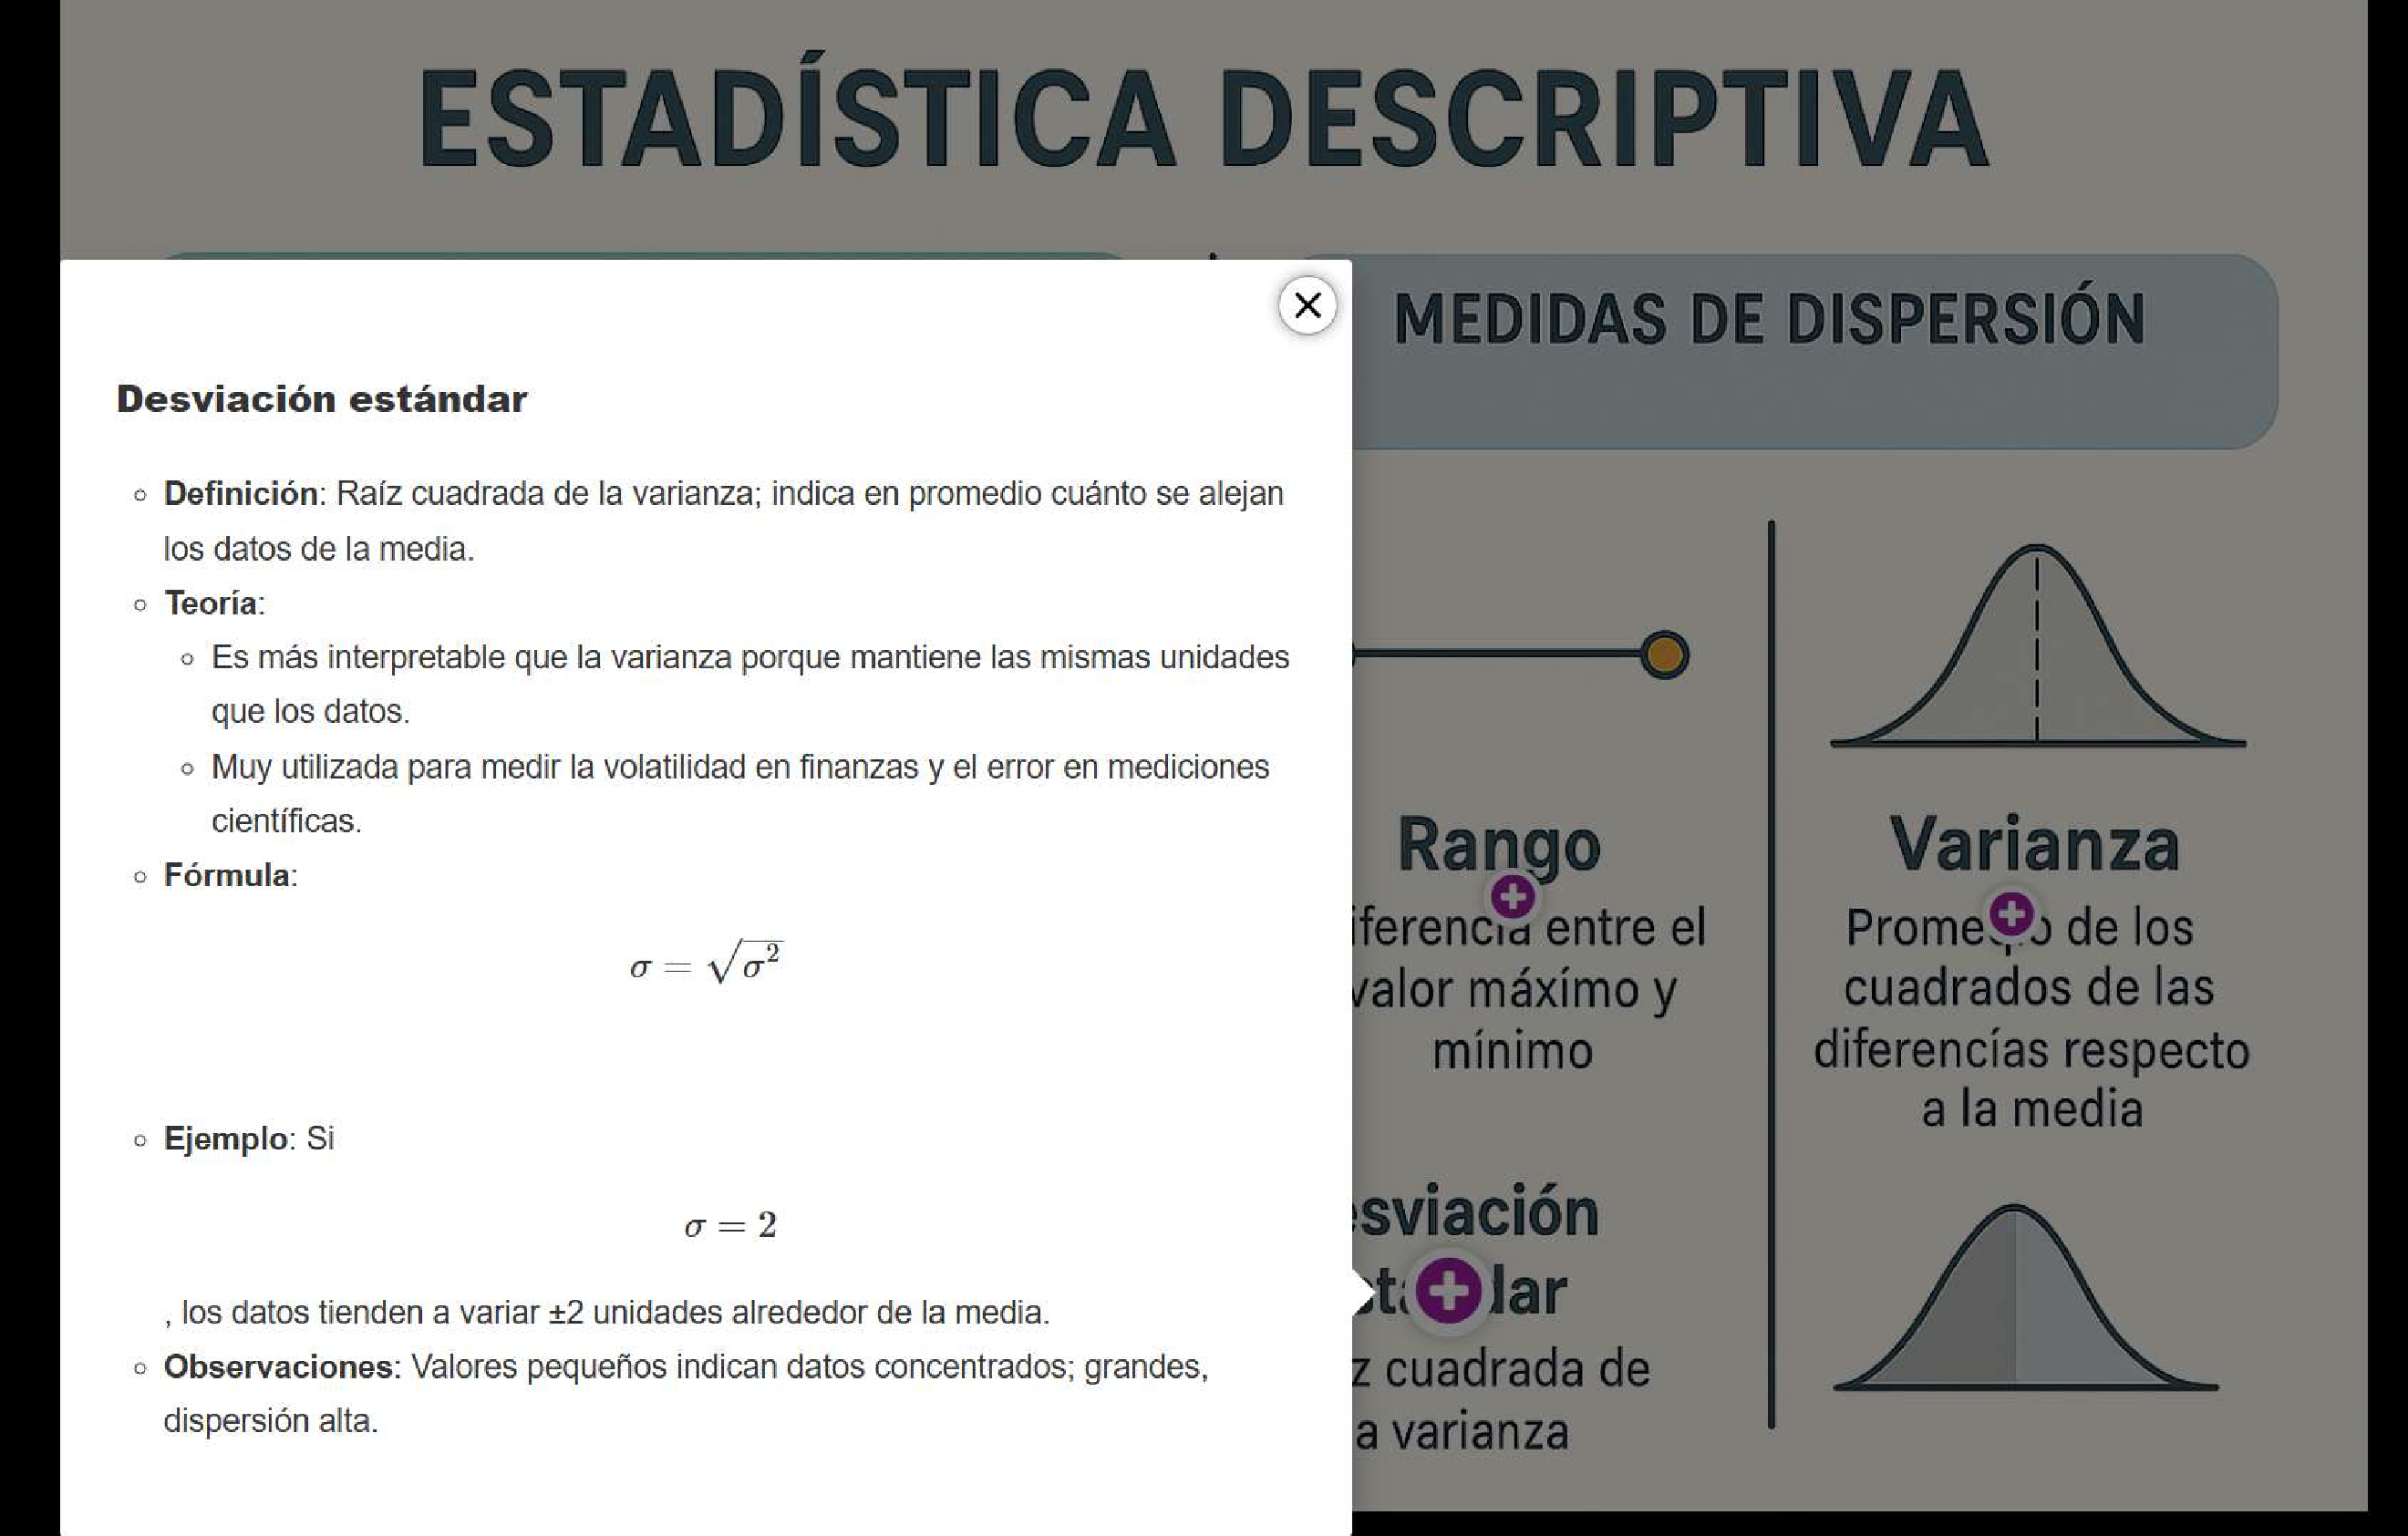
\includegraphics[width=0.85\textwidth]{Figs/Infografia_H5P.pdf}
	\label{fig:H5P}
	\\Fuente: Captura de pantalla de una infografía en H5P.
\end{figure}


Este proceso contó con el acompañamiento del profesor Carlos Mantilla, quien no solo orientó en la correcta implementación de los recursos embebidos, sino que también brindó recomendaciones sobre la manera más efectiva de llevar los temas dentro de \textit{Moodle}.

\section{Experiencia de los Estudiantes}

Un componente clave en la evaluación de resultados fue la percepción de los estudiantes sobre el uso del entorno virtual y las herramientas tecnológicas implementadas. Para este propósito, se aplicó una encuesta a los dos grupos piloto participantes, de la cual respondieron 30 de los 50 estudiantes.

En cuanto al acompañamiento brindado por los practicantes, cerca del $50\%$ de los encuestados consideró que este no fue del todo adecuado, señalando que la orientación recibida no siempre resultó suficiente para resolver sus inquietudes. De manera similar, un $43.3\%$ calificó como \textit{regular} la capacidad del ambiente de aprendizaje para fortalecer la comprensión de los contenidos como se observa en la Figura \ref{fig:Ayuda_Impacto}.

\begin{figure}[h]
	\centering
	\captionof{figure}{\\ \vspace{0.3cm} Experiencia de los Estudiantes. \textbf{Diagramas de: Ayuda de los practicantes y comprensión del contenido}.}
    \begin{subfigure}
        \centering
        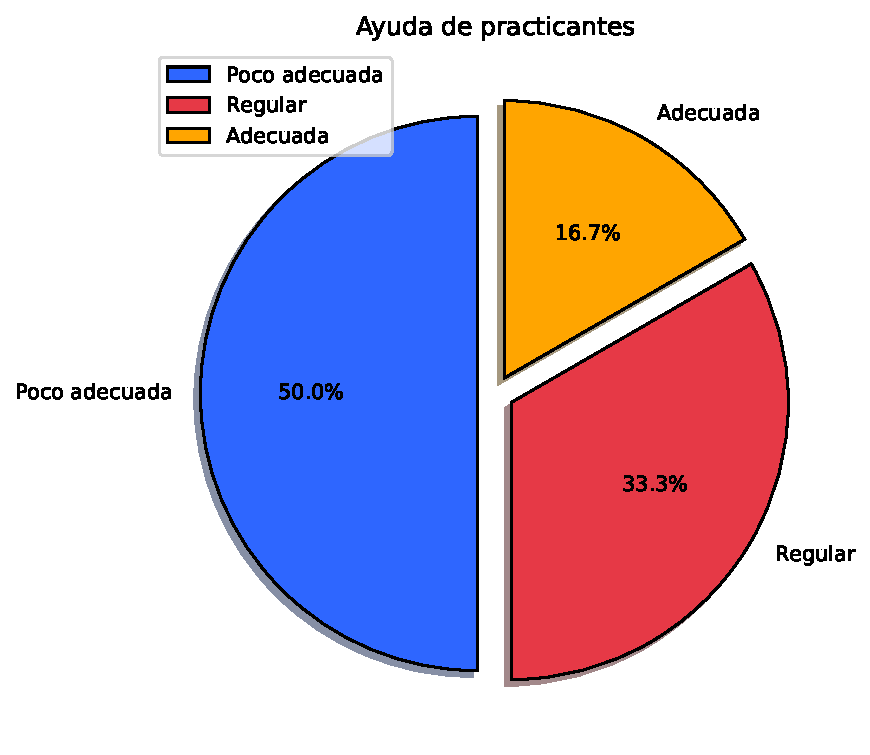
\includegraphics[width=0.40\textwidth]{Figs/ayuda_practicantes.pdf}
    \end{subfigure}
	\hfill
    \begin{subfigure}
        \centering
        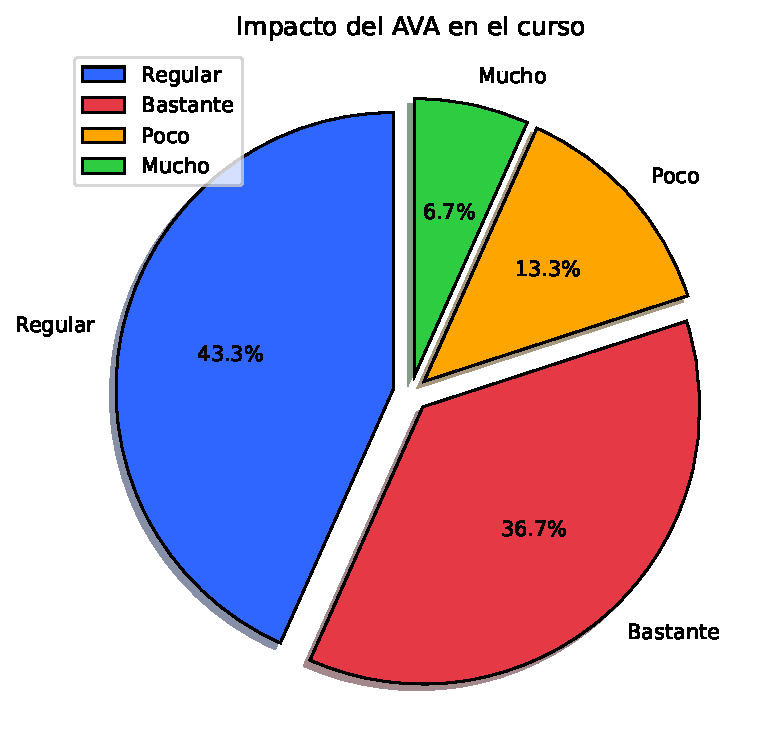
\includegraphics[width=0.37\textwidth]{Figs/impacto_aprendizaje.pdf}
    \end{subfigure}
	\label{fig:Ayuda_Impacto}
	\\ Fuente: Elaboración propia a partir de la encuesta.
\end{figure}

Por otro lado, se resaltaron aspectos positivos relacionados con los métodos de enseñanza utilizados, los cuales fueron valorados como efectivos por el $56.7\%$ de los participantes. A esto se suma la percepción favorable hacia la calidad de los materiales teóricos, que obtuvo una aprobación del $60\%$ Figura \ref{fig:MM}. 

\begin{figure}[h]
	\centering
	\captionof{figure}{\\ \vspace{0.3cm} Experiencia de los Estudiantes. \textbf{Diagramas de los metodos y materiales usados en el curso}.}
    \begin{subfigure}
        \centering
        \includegraphics[width=0.38\textwidth]{Figs/Metodos_Enseñanza.pdf}
    \end{subfigure}
	\hfill
    \begin{subfigure}
        \centering
        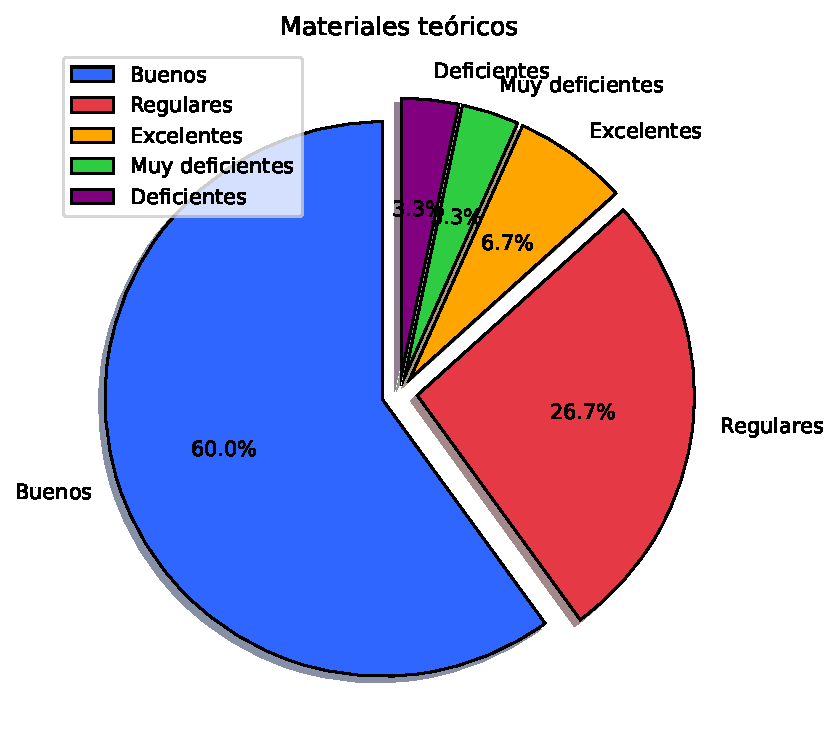
\includegraphics[width=0.38\textwidth]{Figs/materiales_teoricos.pdf}
    \end{subfigure}
	\label{fig:MM}
	\\ Fuente: Elaboración propia a partir de la encuesta.
\end{figure}


Asimismo, los estudiantes reconocieron la rapidez del servidor, con un $73\%$ de aceptación, lo que facilitó el acceso fluido a las actividades y recursos.
Con las herramientas tecnológicas la gran mayoría de los encuestados ($93.3\%$) manifestó su preferencia por Python como lenguaje de programación, argumentando que les resulta más comprensible debido a experiencias previas en otros grupos Figura \ref{fig:RL}. 

\begin{figure}[h]
	\centering
	\captionof{figure}{\\ \vspace{0.3cm} Experiencia de los Estudiantes. \textbf{Diagramas de la respuesta del servidor y el lenguaje preferido}.}
    \begin{subfigure}
        \centering
        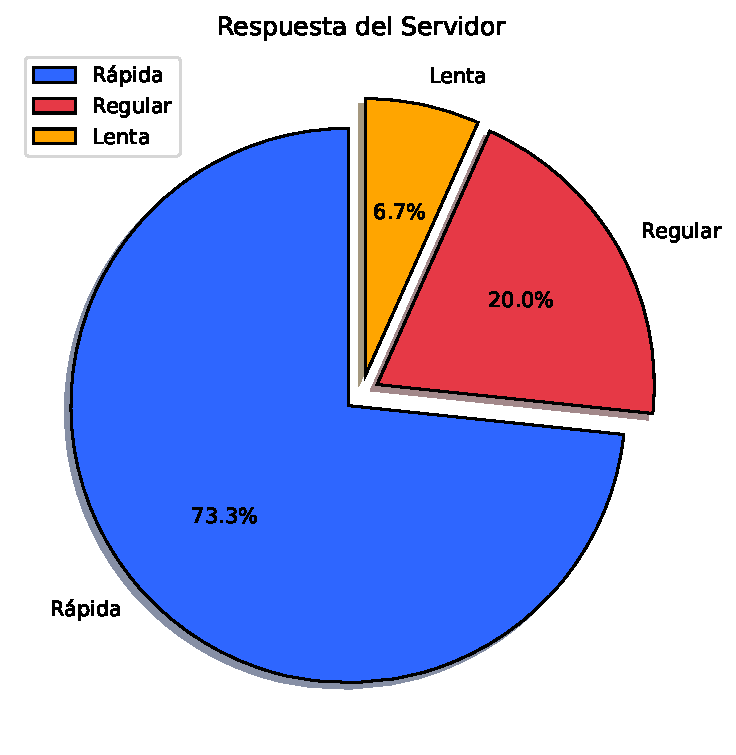
\includegraphics[width=0.38\textwidth]{Figs/Respuesta_Servidor.pdf}
    \end{subfigure}
	\hfill
    \begin{subfigure}
        \centering
        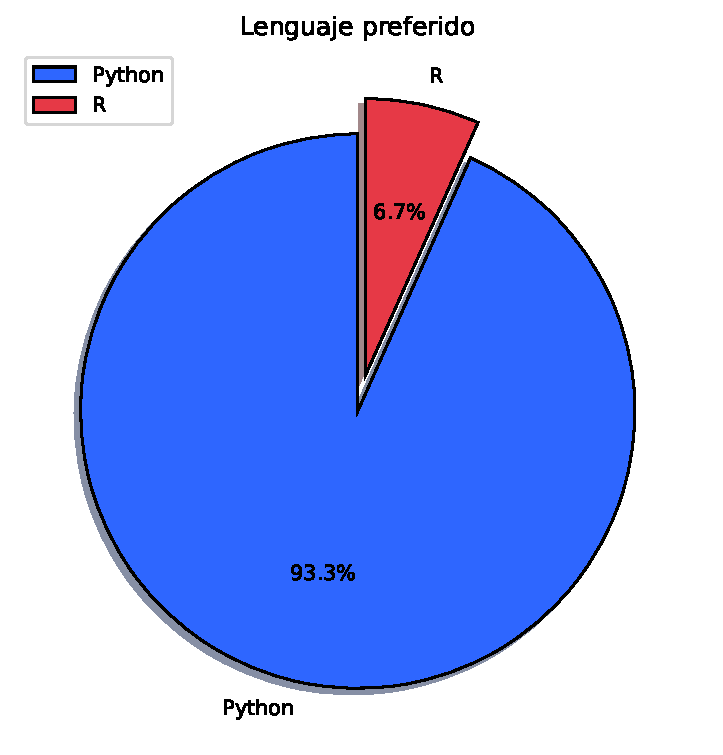
\includegraphics[width=0.38\textwidth]{Figs/lenguaje_preferido.pdf}
    \end{subfigure}
	\label{fig:RL}
	\\ Fuente: Elaboración propia a partir de la encuesta.
\end{figure}

Por otro lado, un porcentaje de ($93.3\%$) resaltó el uso de Google Colab como entorno de programación, destacando que se trata de una herramienta gratuita, de fácil acceso y que no requiere la instalación de programas adicionales.
Pero tambien establecen que es mejor usar las tecnologias implementadas para el desarrollo de el curso de Estadística II teniendo una aceptación del ($63.3\%$) como lo muestra la Figura \ref{fig:CT}.

\begin{figure}[h]
	\centering
	\captionof{figure}{\\ \vspace{0.3cm} Experiencia de los Estudiantes. \textbf{Diagramas del uso de colab y de la integración de tecnologias}.}
    \begin{subfigure}
        \centering
        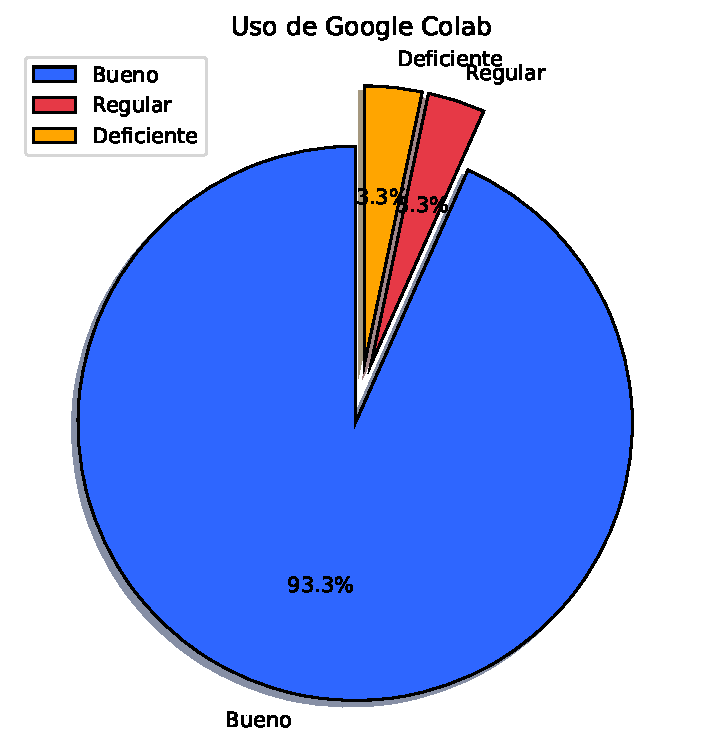
\includegraphics[width=0.355\textwidth]{Figs/uso_colab.pdf}
    \end{subfigure}
	\hfill
    \begin{subfigure}
        \centering
        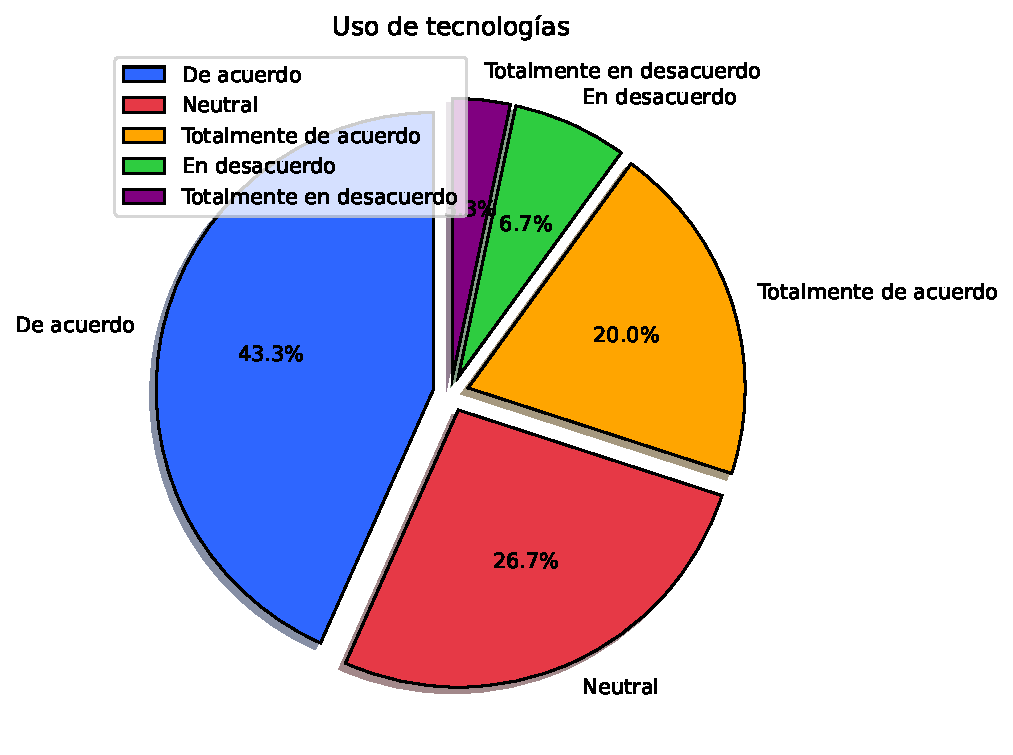
\includegraphics[width=0.475\textwidth]{Figs/uso_tecnologias.pdf}
    \end{subfigure}
	\label{fig:CT}
	\\ Fuente: Elaboración propia a partir de la encuesta.
\end{figure}

No obstante, respecto a la propuesta de consolidar un esquema completo dentro de Moodle que agrupe todos los materiales, el $40\%$ de los estudiantes manifestó estar en desacuerdo y un $56.7\%$ expresó una posición neutral, lo cual refleja que aún existen percepciones divididas frente a la centralización de los recursos Figura \ref{fig:MG}.

Finalmente, el $56.7\%$ de los encuestados coincidieron en que la implementación de evaluadores automáticos (\textit{graders}) fue una herramienta útil para el desarrollo del curso, aportando tanto a la retroalimentación inmediata como a la autoevaluación de los conocimientos adquiridos Figura \ref{fig:MG}.

\begin{figure}[h]
	\centering
	\captionof{figure}{\\ \vspace{0.3cm} Experiencia de los Estudiantes. \textbf{Diagramas sobre centralizar los materiales en Moodle y la implementación de graders}.}
    \begin{subfigure}
        \centering
        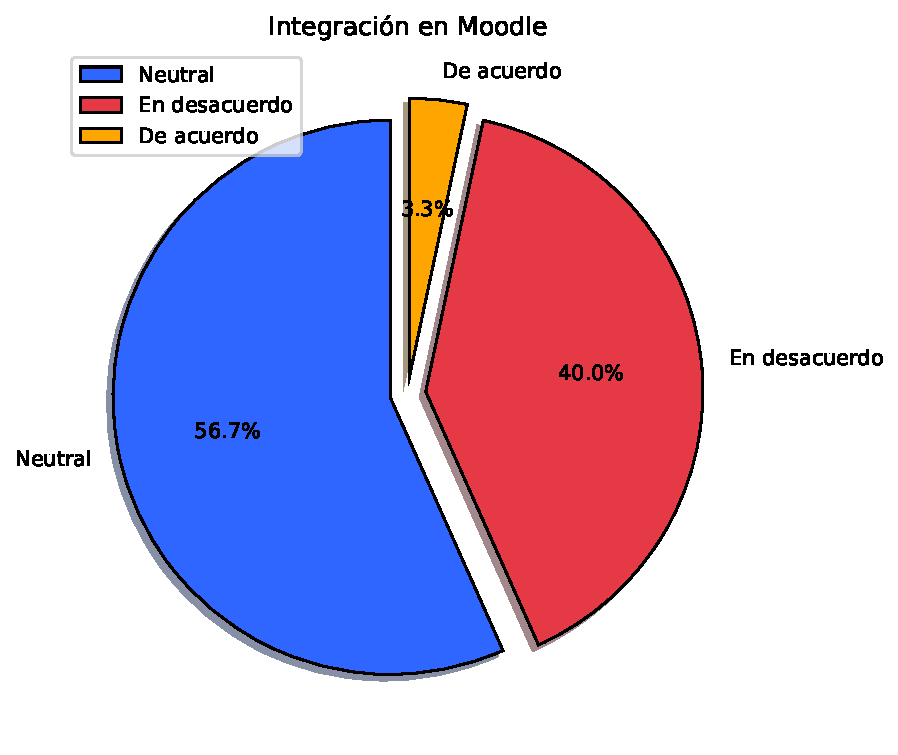
\includegraphics[width=0.4\textwidth]{Figs/integracion_moodle.pdf}
    \end{subfigure}
	\hfill
    \begin{subfigure}
        \centering
        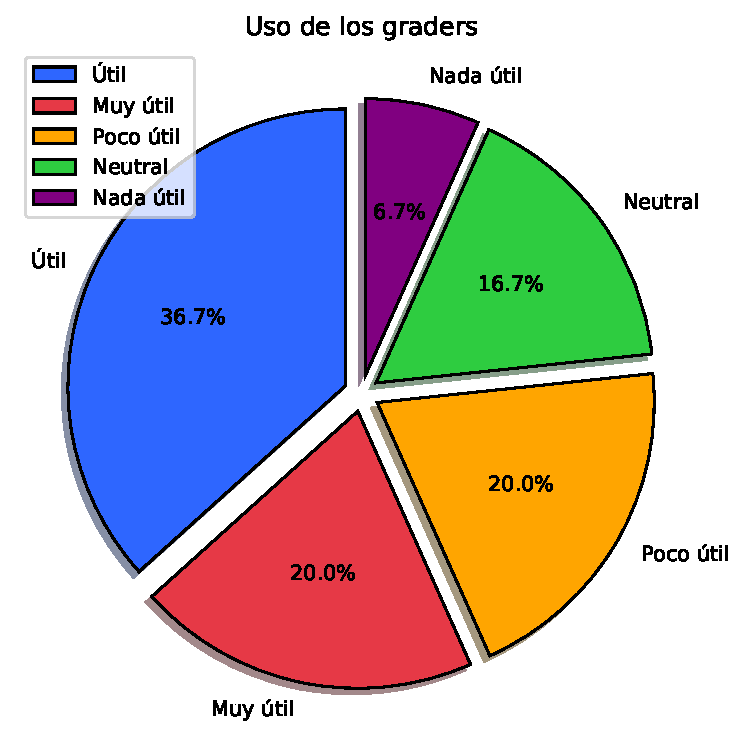
\includegraphics[width=0.35\textwidth]{Figs/uso_graders.pdf}
    \end{subfigure}
	\label{fig:MG}
	\\ Fuente: Elaboración propia a partir de la encuesta.
\end{figure}

\newpage

\section{Análisis de los grupos piloto}

Se hizo el análisis de cinco prácticas de laboratorio en los grupos piloto, los cuales evidencian una evolución desigual en el proceso de aprendizaje de los estudiantes. También, se analizó tanto el código entregado por los estudiantes (Anexo \ref{anexo:repositorio}), como su nivel de atención durante las clases, con el propósito de identificar si la falta de concentración o el uso inadecuado de recursos externos podía influir en la calidad de las soluciones presentadas. 

En la \textbf{Práctica 1} se presentó la mayor dificultad inicial: el  promedio es de $\bar{x}=2.17$, con una mediana de $2.18$, una desviación estándar de $\sigma=1.44$ y un rango intercuartílico $\text{IQR}$ de $2.23$. Estos indicadores reflejan un bajo desempeño general y una gran dispersión en los resultados, como se muestra en la Figura \ref{fig:Mapa}.

La \textbf{Práctica 2} marcó un avance notable en el rendimiento, con un promedio de $\bar{x}=3.89$, mediana de $4.27$, desviación estándar de $\sigma=1.47$ e $\text{IQR}$ de $1.67$. Este progreso se refleja también en la Figura \ref{fig:Dispersion}, donde se observa una concentración importante de calificaciones entre $4.0$ y $5.0$.

La \textbf{Práctica 3} representó el punto más alto del proceso formativo, alcanzando un promedio de $\bar{x}=4.14$, una mediana de $4.5$, desviación estándar de $\sigma=1.13$ e $\text{IQR}$ de $1.28$. Estos resultados muestran homogeneidad y predominio de notas altas, lo que sugiere que en este momento del curso los estudiantes lograron consolidar de manera más efectiva sus aprendizajes.

No obstante, en la \textbf{Práctica 4} ($\bar{x}=3.92$, mediana $4.33$, desviación estándar $\sigma=1.62$, $\text{IQR}$ $1.46$) y, sobre todo, en la \textbf{Práctica 5} ($\bar{x}=2.24$, mediana $2.80$, desviación estándar $\sigma=1.54$, $\text{IQR}$ $3.42$), se evidencia un retroceso importante. En esta última práctica, la Figura \ref{fig:Promedio} muestra una caída significativa de la mediana y una alta dispersión, mientras que la Figura \ref{fig:Dispersion} confirma la concentración de notas bajas, convirtiéndola en la actividad más crítica del proceso.

\begin{figure}[ht]
	\centering
	\captionof{figure}{ \\ \vspace{0.5cm} Análisis de los grupos piloto. \textbf{Diagrama de dispersión de notas de las prácticas}.}
	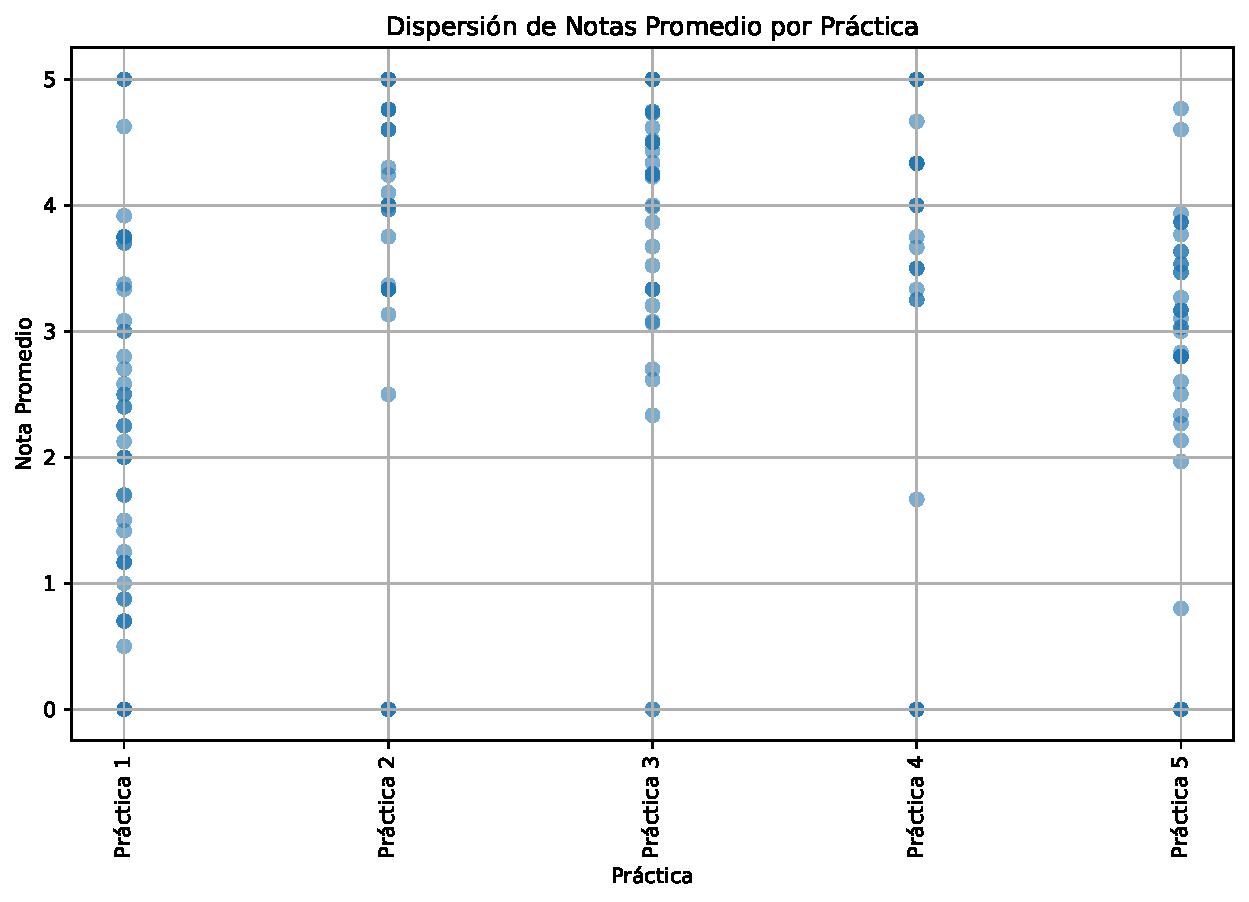
\includegraphics[width=0.9\textwidth]{Figs/Dispersion_Notas.pdf}
	\label{fig:Dispersion}
	\\Fuente: Elaboración propia a partir de las notas de las prácticas 1 a 5.
\end{figure}

Los resultados sugieren que los estudiantes son capaces de alcanzar altos niveles de rendimiento cuando cuentan con condiciones de práctica dirigida, retroalimentación inmediata o acompañamiento cercano, como se reflejó en las Prácticas 2, 3 y 4 evidenciado en la Figura \ref{fig:Mapa}. Sin embargo, el retroceso evidenciado en la Práctica 5 revela que, cuando el proceso depende más del aprendizaje autónomo y de la aplicación de la teoría, aparecen varias dificultades.

De acuerdo con las prácticas no se puede explicar únicamente la complejidad de las actividades, sino también por factores comportamentales y pedagógicos. Se observó que algunos estudiantes no prestan la atención adecuada en las clases, se distraen con los celulares o confían en el uso de herramientas como la IA y en la posibilidad de tener más de un intento para resolver las actividades. No obstante, los resultados demuestran que esta dependencia no compensa la falta de comprensión conceptual; cuando las tareas exigen aplicar ecuaciones o integrar teoría en código, muchos estudiantes no logran resolverlas de forma adecuada o, en ciertos casos, deciden no presentar las actividades.

\begin{figure}[ht]
	\centering
	\captionof{figure}{ \\ \vspace{0.5cm} Análisis de los grupos piloto. \textbf{Diagrama de boxplots de notas de las prácticas}.}
	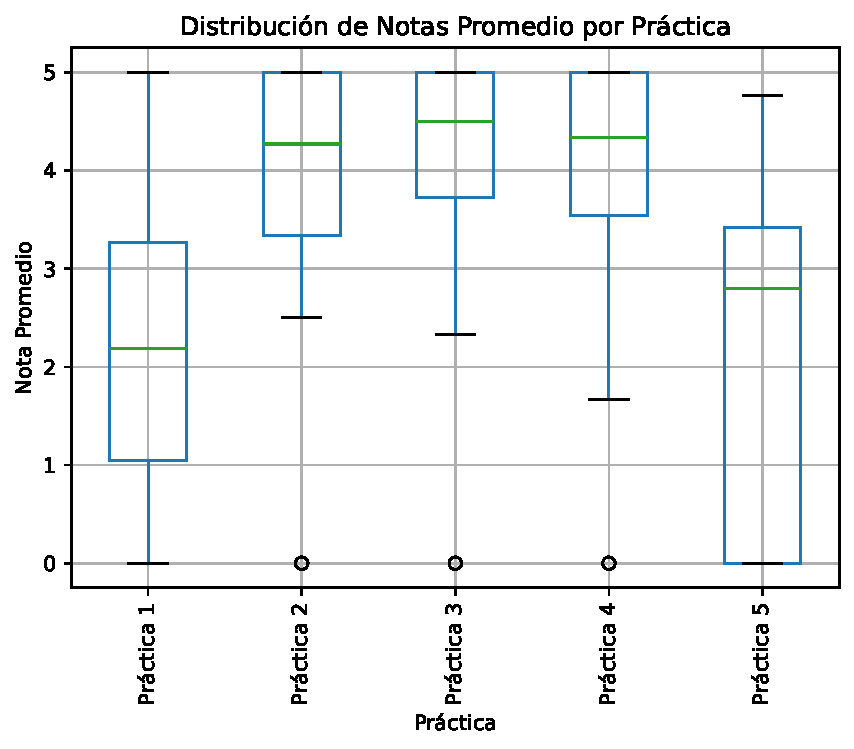
\includegraphics[width=0.9\textwidth]{Figs/Promedio_Notas.pdf}
	\label{fig:Promedio}
	\\Fuente: Elaboración propia a partir de las notas de las prácticas 1 a 5.
\end{figure}

\begin{figure}[ht]
	\centering
	\captionof{figure}{ \\ \vspace{0.5cm} Análisis de los grupos piloto. \textbf{Diagrama de matriz de correlación de notas de las prácticas}.}
	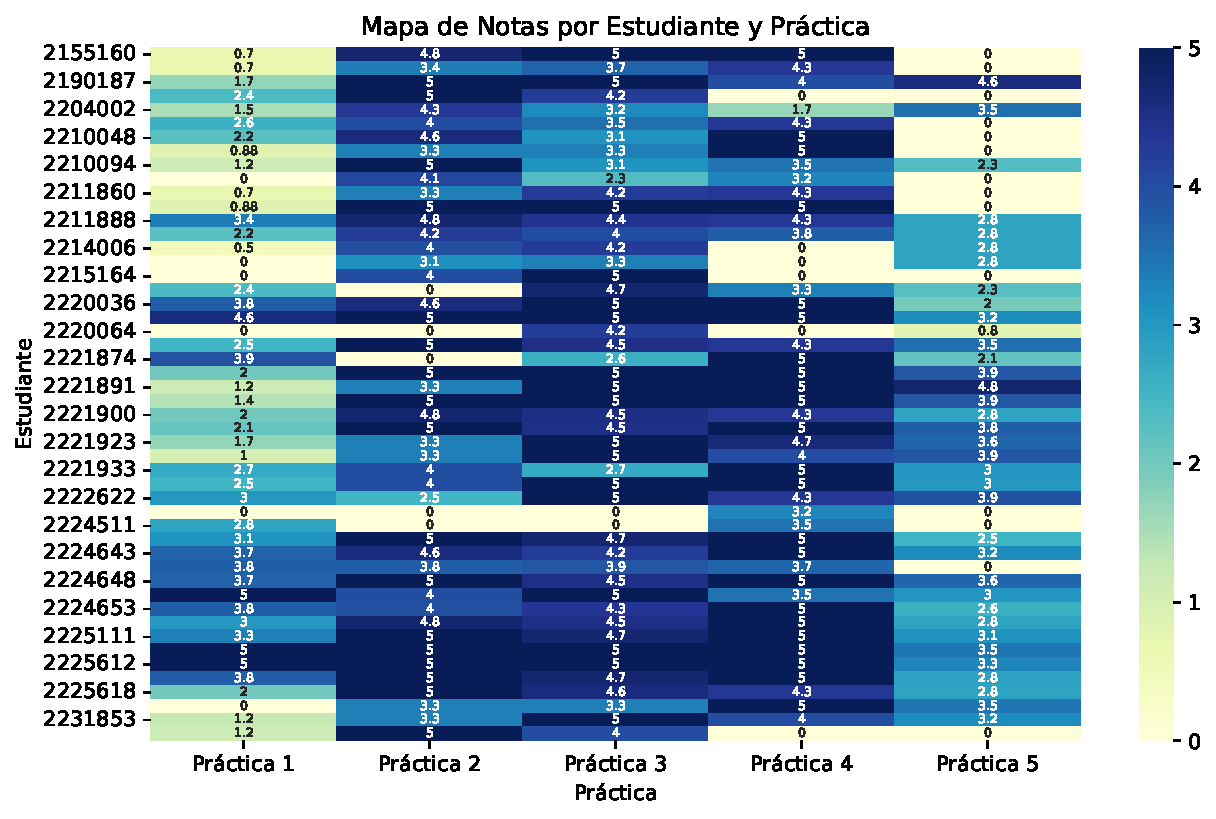
\includegraphics[width=1\textwidth]{Figs/Mapa_Notas.pdf}
	\label{fig:Mapa}
	\\Fuente: Elaboración propia a partir de las notas de las prácticas 1 a 5.
\end{figure}

\section{Generalización de los resultados}

Los resultados obtenidos evidencian que los estudiantes aprovecharon de manera significativa las herramientas tecnológicas disponibles en el aula virtual para apoyar la solución de problemas relacionados con la asignatura y con situaciones prácticas de su formación. Sin embargo, también se identificó que no todos hicieron un uso responsable de estos recursos. En algunos casos, de no haberse implementado medidas de control como el uso del \textit{Safe Exam Browser (SEB)} y otras estrategias de acompañamiento docente, los estudiantes habrían recurrido de forma excesiva a herramientas externas, como la inteligencia artificial, para resolver actividades, prácticas e incluso cuestionarios. Esto condujo a situaciones en las que se emplearon librerías y métodos no explicados en clase, lo que ocasionó inconsistencias en el aprendizaje y resultados poco confiables en el \textit{autocalificador}, reflejados en calificaciones desfavorables.

No obstante, este panorama también dejó en evidencia aspectos muy positivos. Los estudiantes que asumieron con compromiso y esfuerzo su proceso de aprendizaje lograron aprovechar al máximo los contenidos interactivos y las herramientas de programación integradas en el AVA. Asimismo, se beneficiaron del acompañamiento de los practicantes, quienes desempeñaron un papel clave en la resolución de dudas y en la orientación del uso adecuado de los recursos.

Estos resultados mostraron dos realidades distintas, donde por un lado, ponen de manifiesto la importancia de fortalecer los mecanismos de control y el acompañamiento docente, para de evitar el uso inadecuado de recursos externos. Pero, al mismo tiempo, muestran el gran potencial que tiene el ambiente virtual cuando los estudiantes lo asumen con responsabilidad y compromiso.

En términos de gestión, se evidencia que la infraestructura tecnológica (\textit{Docker}, \textit{Node.js}, \textit{MariaDB}, \textit{Nginx}, \textit{Playit.gg}) y los recursos pedagógicos (\textit{H5P}, \textit{Genially}, \textit{iframes}, \textit{SEB}) aportaron a la consolidación de un entorno seguro, dinámico y accesible.

Finalmente, se destaca que todo lo implementado se encuentra documentado en el Anexo \ref{anexo:repositorio}, donde se detallan desde la infraestructura tecnológica, los \textit{graders} y el material teórico interactivo desarrollado para el curso. Este soporte documental no solo respalda la implementación realizada, sino que también garantiza su posible replicabilidad en otros espacios académicos.


\newpage

\chapter{Conclusiones y trabajo a futuro}

\section{Conclusiones}

En el presente trabajo se evidenció que los estudiantes aprovecharon de manera significativa las herramientas tecnológicas integradas en el entorno virtual (\textit{Colab Notebooks}, Python, R, H5P y Genially) para resolver problemas relacionados con la asignatura y con situaciones prácticas de su formación. La implementación de contenidos interactivos, infografías, presentaciones y ejercicios con retroalimentación inmediata permitió consolidar un aprendizaje activo y práctico, alineado con los objetivos del curso de Estadística II.

Se diseñó un plan de aula modular que permitió estructurar los contenidos teóricos y prácticos de manera coherente en notebooks de Colab, utilizando los dos lenguajes propuestos (Python y R). Estos notebooks estaban configurados con autocalificación, lo que generaba una nota y a su vez, facilitaba que los estudiantes recibieran retroalimentación inmediata en función del trabajo realizado. Los resultados obtenidos en los cursos piloto evidenciaron que el plan fue apropiado y progresivo, ya que se reflejó una curva de aprendizaje ascendente durante el pilotaje: la Práctica 1 presentó un promedio de 2,17, la Práctica 3 alcanzó 4,14, mientras que el promedio global de las cinco prácticas analizadas fue 3,27. No obstante, en la Práctica 5 se observó un retroceso significativo ($\bar{x}$ = 2,24), lo cual sugiere la necesidad de ajustar aspectos metodológicos en fases posteriores. Estos resultados confirman tanto la pertinencia del diseño como su nivel de dificultad adecuado para fomentar un aprendizaje progresivo, aunque con retos que requieren intervención pedagógica continua.

El ambiente virtual de aprendizaje (AVA) implementado en Moodle integró de manera efectiva el contenido teórico y práctico del curso, evidenciando su utilidad tanto como espacio formativo como herramienta de seguimiento y retroalimentación. En el caso de los cuestionarios, el primer ejercicio evaluativo presentó un promedio de 2.6 sobre 5, lo cual permitió identificar de manera temprana las dificultades en la apropiación de los conceptos. Al mismo tiempo, la percepción estudiantil respaldó la pertinencia de la propuesta donde el 73.3\% calificó la respuesta del servidor como rápida, el 93.3\% manifestó preferencia por Python y el 93.3\% valoró positivamente el uso de Google Colab. Estos resultados confirman la eficacia técnica y pedagógica del AVA, fortaleciendo su papel en el proceso de enseñanza-aprendizaje.

El AVA se implementó en dos grupos de la asignatura Estadística II de la Escuela de Ingeniería de Sistemas e Informática (C1 y F3), bajo la dirección del profesor Andrés Leonardo González Gómez, quien autorizó su uso para el pilotaje del ambiente virtual. Durante este proceso se evidenció una mejora progresiva en el desempeño académico de los estudiantes. El promedio inicial en la Práctica 1 fue de 2.17, mientras que en la Práctica 3 se alcanzó un promedio de 4.14, lo que corresponde a un incremento aproximado del 91\% en relación con el punto de partida. Considerando el conjunto de las cinco prácticas realizadas, el promedio global fue de 3.27, valor que refleja una mejora global del 51\% frente al rendimiento inicial y evidencia la adaptación progresiva de los estudiantes, aunque con retrocesos puntuales en la última práctica que ponen de manifiesto la necesidad de fortalecer estrategias metodológicas.

No obstante, se identificó que no todos los estudiantes hicieron un uso adecuado de herramientas externas como la inteligencia artificial. Aunque en algunos casos se implementó el plugin Safe Exam Browser (SEB) y estrategias de acompañamiento para los cuestionarios y evaluaciones, estas medidas no fueron suficientes en las actividades tipo laboratorio, donde en la práctica 5 se presentó un aproximado del 56\% de los estudiantes del grupo piloto hicieron uso de IA, evidenciado en errores de formato, la aplicación de métodos no explicados en clase y la utilización de librerías que resolvían los problemas estadísticos sin necesidad de aplicar las fórmulas correspondientes.

Finalmente la encuesta aplicada a los estudiantes permitió concluir que el ambiente virtual de aprendizaje fue valorado de manera positiva en términos de rapidez, pertinencia pedagógica y uso de herramientas tecnológicas, destacándose la preferencia por Python y Google Colab. Asimismo, la mayoría de los participantes reconoció que el AVA contribuyó al fortalecimiento de su comprensión en Estadística II, lo que confirma su impacto como apoyo metodológico y tecnológico en el proceso de enseñanza-aprendizaje.

\section{Trabajo a futuro}

Se recomienda ampliar el uso del entorno virtual no solo a más grupos de Estadística II, sino también a otras asignaturas de la Escuela de Ingeniería de Sistemas e Informática. De esta forma, sería posible evaluar su escalabilidad y comprobar su efectividad en distintos contextos de enseñanza.

En cuanto a los instrumentos de evaluación, es conveniente optimizarlos incorporando una mayor diversidad de ejercicios prácticos y autoevaluativos, junto con métricas que permitan un seguimiento más detallado y personalizado del progreso de cada estudiante.

Si bien el uso de \textit{Safe Exam Browser (SEB)} y otras estrategias resultó positivo, se considera necesario explorar nuevos mecanismos de supervisión y acompañamiento que fortalezcan el uso responsable de los recursos digitales y prevengan conductas que puedan comprometer la integridad académica.

Asimismo, la implementación del aula modular en Moodle habría sido mucho más sencilla si hubiese sido posible integrar diferentes plugins orientados a la contenerización mediante Docker y a la gestión de los \textit{graders}. De esta manera, los servicios podrían haberse expuesto directamente desde la plataforma, lo cual representaría una mejora importante en la implementación de proyectos de este tipo.

Finalmente, se sugiere incrementar la cantidad de actividades interactivas, infografías dinámicas y ejercicios de simulación en Python y R. Estas acciones no solo favorecerían la práctica constante, sino que también impulsarían la aplicación de los conceptos estadísticos en problemas más complejos y cercanos a la realidad profesional, contribuyendo a un aprendizaje más profundo y significativo.

\newpage
% ------------------------------------------------------------------------
% Bibliografía
% ------------------------------------------------------------------------

%\addcontentsline{toc}{chapter}{Referencias Bibliográficas}\newpage
%\bibliographystyle{apalike}
%\bibliography{biblio}
\addcontentsline{toc}{chapter}{Referencias Bibliográficas}

\printbibliography

\nocite{poniszewska-maranda, burns-kubernetes, torres-bosch-microservicios, armstrong2015,kubevirtio, docker2023, kubelet-doc, namespace-article}
% ------------------------------------------------------------------------
% Anexos
\newpage

\bgroup
\bgroup
\makeatletter
\@openrightfalse
\appendix

% --- Solo una entrada en la TOC ---
\chapter*{Anexos}
\addcontentsline{toc}{chapter}{Anexos}

% --- Anexo 1 ---
\refstepcounter{chapter}
\chapter*{Anexo \thechapter: Actas de reunión}
\label{anexo:actas}

\section*{Acta de reunión inicial - 02 de abril de 2025}
\label{anexo:acta-abril-2025}

\foreach \p in {1,...,5}{ % número de páginas del PDF
	\begin{figure}[H]
		\centering
		\includegraphics[page=\p, width=1.8\textwidth, height=0.765\textheight, keepaspectratio]{Anexos/Acta 02 abril de 2025.pdf}
	\end{figure}
}

\newpage

% --- Anexo 2 ---
\refstepcounter{chapter}
\chapter*{Anexo \thechapter: Guías de prácticas}
\label{anexo:Guía-Semana-8}

\section*{Guía de práctica de la semana 8}
\label{anexo:guia-semana-8}

\foreach \p in {1,...,2}{ % número de páginas del PDF
	\begin{figure}[H]
		\centering
		\includegraphics[page=\p, width=1.8\textwidth, height=0.765\textheight, keepaspectratio]{Anexos/G.pdf}
	\end{figure}
}

\newpage

% --- Anexo 3 ---
\refstepcounter{chapter}
\chapter*{Anexo \thechapter: Repositorio del Proyecto}
\label{anexo:repositorio}

El código fuente de este proyecto se encuentra disponible en el repositorio público:

\begin{center}
\href{https://github.com/JorEdu33/Estructura-del-servidor-y-Material-de-clase.git}{\texttt{https://github.com/JorEdu33/Estructura-del-servidor-y-Material-de-clase.git}}
\end{center}

\makeatother
\egroup

% ------------------------------------------------------------------------

% ------------------------------------------------------------------------
\end{document}                                          % Fin de documento
% ------------------------------------------------------------------------ 
